%!TEX root=./LIVRO.tex
\chapter{CORRIDA DOS NÚMEROS}
\markboth{Módulo 1}{}

%\coment{Neste módulo, vamos trabalhar com os alunos as habilidades referentes à manipulação dos algarismos, de modo que o aluno consiga formar, ordenar e utilizar alguns números, de até 3 ordens, em diversas aplicações de contagem, ordenação e identificação.}

\section*{HABILIDADES DO SAEB}

\begin{itemize}
\item
  \uppercase{Reconhecer o que os números naturais indicam em diferentes situações:
  quantidade, ordem, medida ou código de identificação.}
\item
  \uppercase{Identificar a posição ordinal de um objeto ou termo em uma sequência
  (1º, 2º etc.).}
\item
  \uppercase{Escrever números naturais de até 3 ordens em sua representação por
  algarismos ou em língua materna ou associar o registro numérico de
  números naturais de até 3 ordens ao registro em língua materna.}
\item
  \uppercase{Comparar ou ordenar quantidades de objetos (até 2 ordens).}
\item
  \uppercase{Comparar ou ordenar números naturais de até 3 ordens com ou sem
  suporte da reta numérica.}
\item
  \uppercase{Identificar a ordem ocupada por um algarismo ou seu valor posicional
  (ou valor relativo) em um número natural de até 3 ordens.}
\end{itemize}

\subsection{HABILIDADES DA BNCC}

\begin{itemize}
  \item EF01MA01, EF01MA03, EF01MA05.
\end{itemize}

\conteudo{
OS AMIGOS DO CONDOMÍNIO DE JOÃO RESOLVERAM FAZER UMA CORRIDA COM SEUS
CARRINHOS. HAVIA \textbf{QUINZE} GAROTOS, E CADA UM DELES TROUXE
\textbf{UM} CARRINHO PARA A CORRIDA.


QUEM CHEGARÁ EM
\textbf{PRIMEIRO} LUGAR? QUEM CHEGARÁ EM \textbf{SEGUNDO}
LUGAR? QUEM COMPLETARÁ O PÓDIO, NO \textbf{TERCEIRO} LUGAR?
PARA MELHORAR O CONTROLE DA CORRIDA, OS MENINOS RESOLVERAM CODIFICAR
CADA CARRINHO COM UM NÚMERO.


JOÃO, QUE FOI QUEM TEVE A IDEIA DA CORRIDA,
TRATOU LOGO DE ESCOLHER O NÚMERO DE SEU PILOTO FAVORITO DE FÓRMULA 1. OS
OUTROS MENINOS ESCOLHERAM NÚMEROS DE QUE ELES GOSTAVAM. UM ERA O CARRO
\textbf{44}, OUTRO ERA O CARRO \textbf{12}, POR EXEMPLO.

VOCÊ PERCEBEU COMO USAMOS OS NÚMEROS DE DIVERSAS FORMAS? ELES FORAM
ÚTEIS PARA NOS AJUDAR A CONTAR OS CARROS E A QUANTIDADE DE PARTICIPANTES
DA CORRIDA. ELES TAMBÉM NOS AJUDARAM A DEFINIR A CLASSIFICAÇÃO DOS
CORREDORES, E ATÉ NOS INDICARAM O VENCEDOR, OU SEJA, O PRIMEIRO A CRUZAR
A LINHA DE CHEGADA. ALÉM DISSO, OS NÚMEROS NÃO SERVEM SOMENTE PARA
CONTARMOS, MAS TAMBÉM PARA IDENTIFICARMOS ALGO.


OS
AMIGOS CORREDORES DERAM NÚMEROS DE IDENTIFICAÇÃO A SEUS CARROS.
NOSSAS CASAS TAMBÉM TÊM NÚMEROS. ESSE É MAIS UM EXEMPLO DE
NÚMEROS SERVINDO PARA IDENTIFICAR EM VEZ DE CONTAR.
}

\section*{ATIVIDADES}

\num{1} CIRCULE A FIGURA QUE CONTÉM UM NÚMERO USADO COMO CÓDIGO DE IDENTIFICAÇÃO.

%\textless{}https://stock.adobe.com/br/images/id/363300782?get\_facets=1\&order=relevance\&safe\_search=1\&k=r\%C3\%A9gua\&clickref=1100lwwNzM24\&mv=affiliate\&mv2=Freepik\&as\_camptype=\&as\_channel=affiliate\&as\_source=partnerize\&as\_campaign=Freepik\&as\_content=api\&as\_audience=srp\&sdid=6WTV6YJ5; https://stock.adobe.com/br/search?load\_type=search\&is\_recent\_search=\&search\_type=usertyped\&k=NUMERO+DE+CASA\&native\_visual\_search=\&similar\_content\_id=\&asset\_id=506848063; https://stock.adobe.com/br/search?filters\%5Bcontent\_type\%3Aphoto\%5D=1\&filters\%5Bcontent\_type\%3Aillustration\%5D=1\&filters\%5Bcontent\_type\%3Azip\_vector\%5D=1\&filters\%5Bcontent\_type\%3Avideo\%5D=1\&filters\%5Bcontent\_type\%3Atemplate\%5D=1\&filters\%5Bcontent\_type\%3A3d\%5D=1\&filters\%5Bcontent\_type\%3Aimage\%5D=1\&order=relevance\&safe\_search=1\&limit=100\&search\_page=1\&k=1+KG\&search\_type=usertyped\&acp=\&aco=1+KG\&get\_facets=0\&asset\_id=418803262. Inserir um diagrama com as 4 figuras, conforme modelo a seguir. É importante que as imagens tenham um tamanho grande, para que os alunos consigam enxergar os números.\textgreater{}

\begin{figure}[H]
\centering
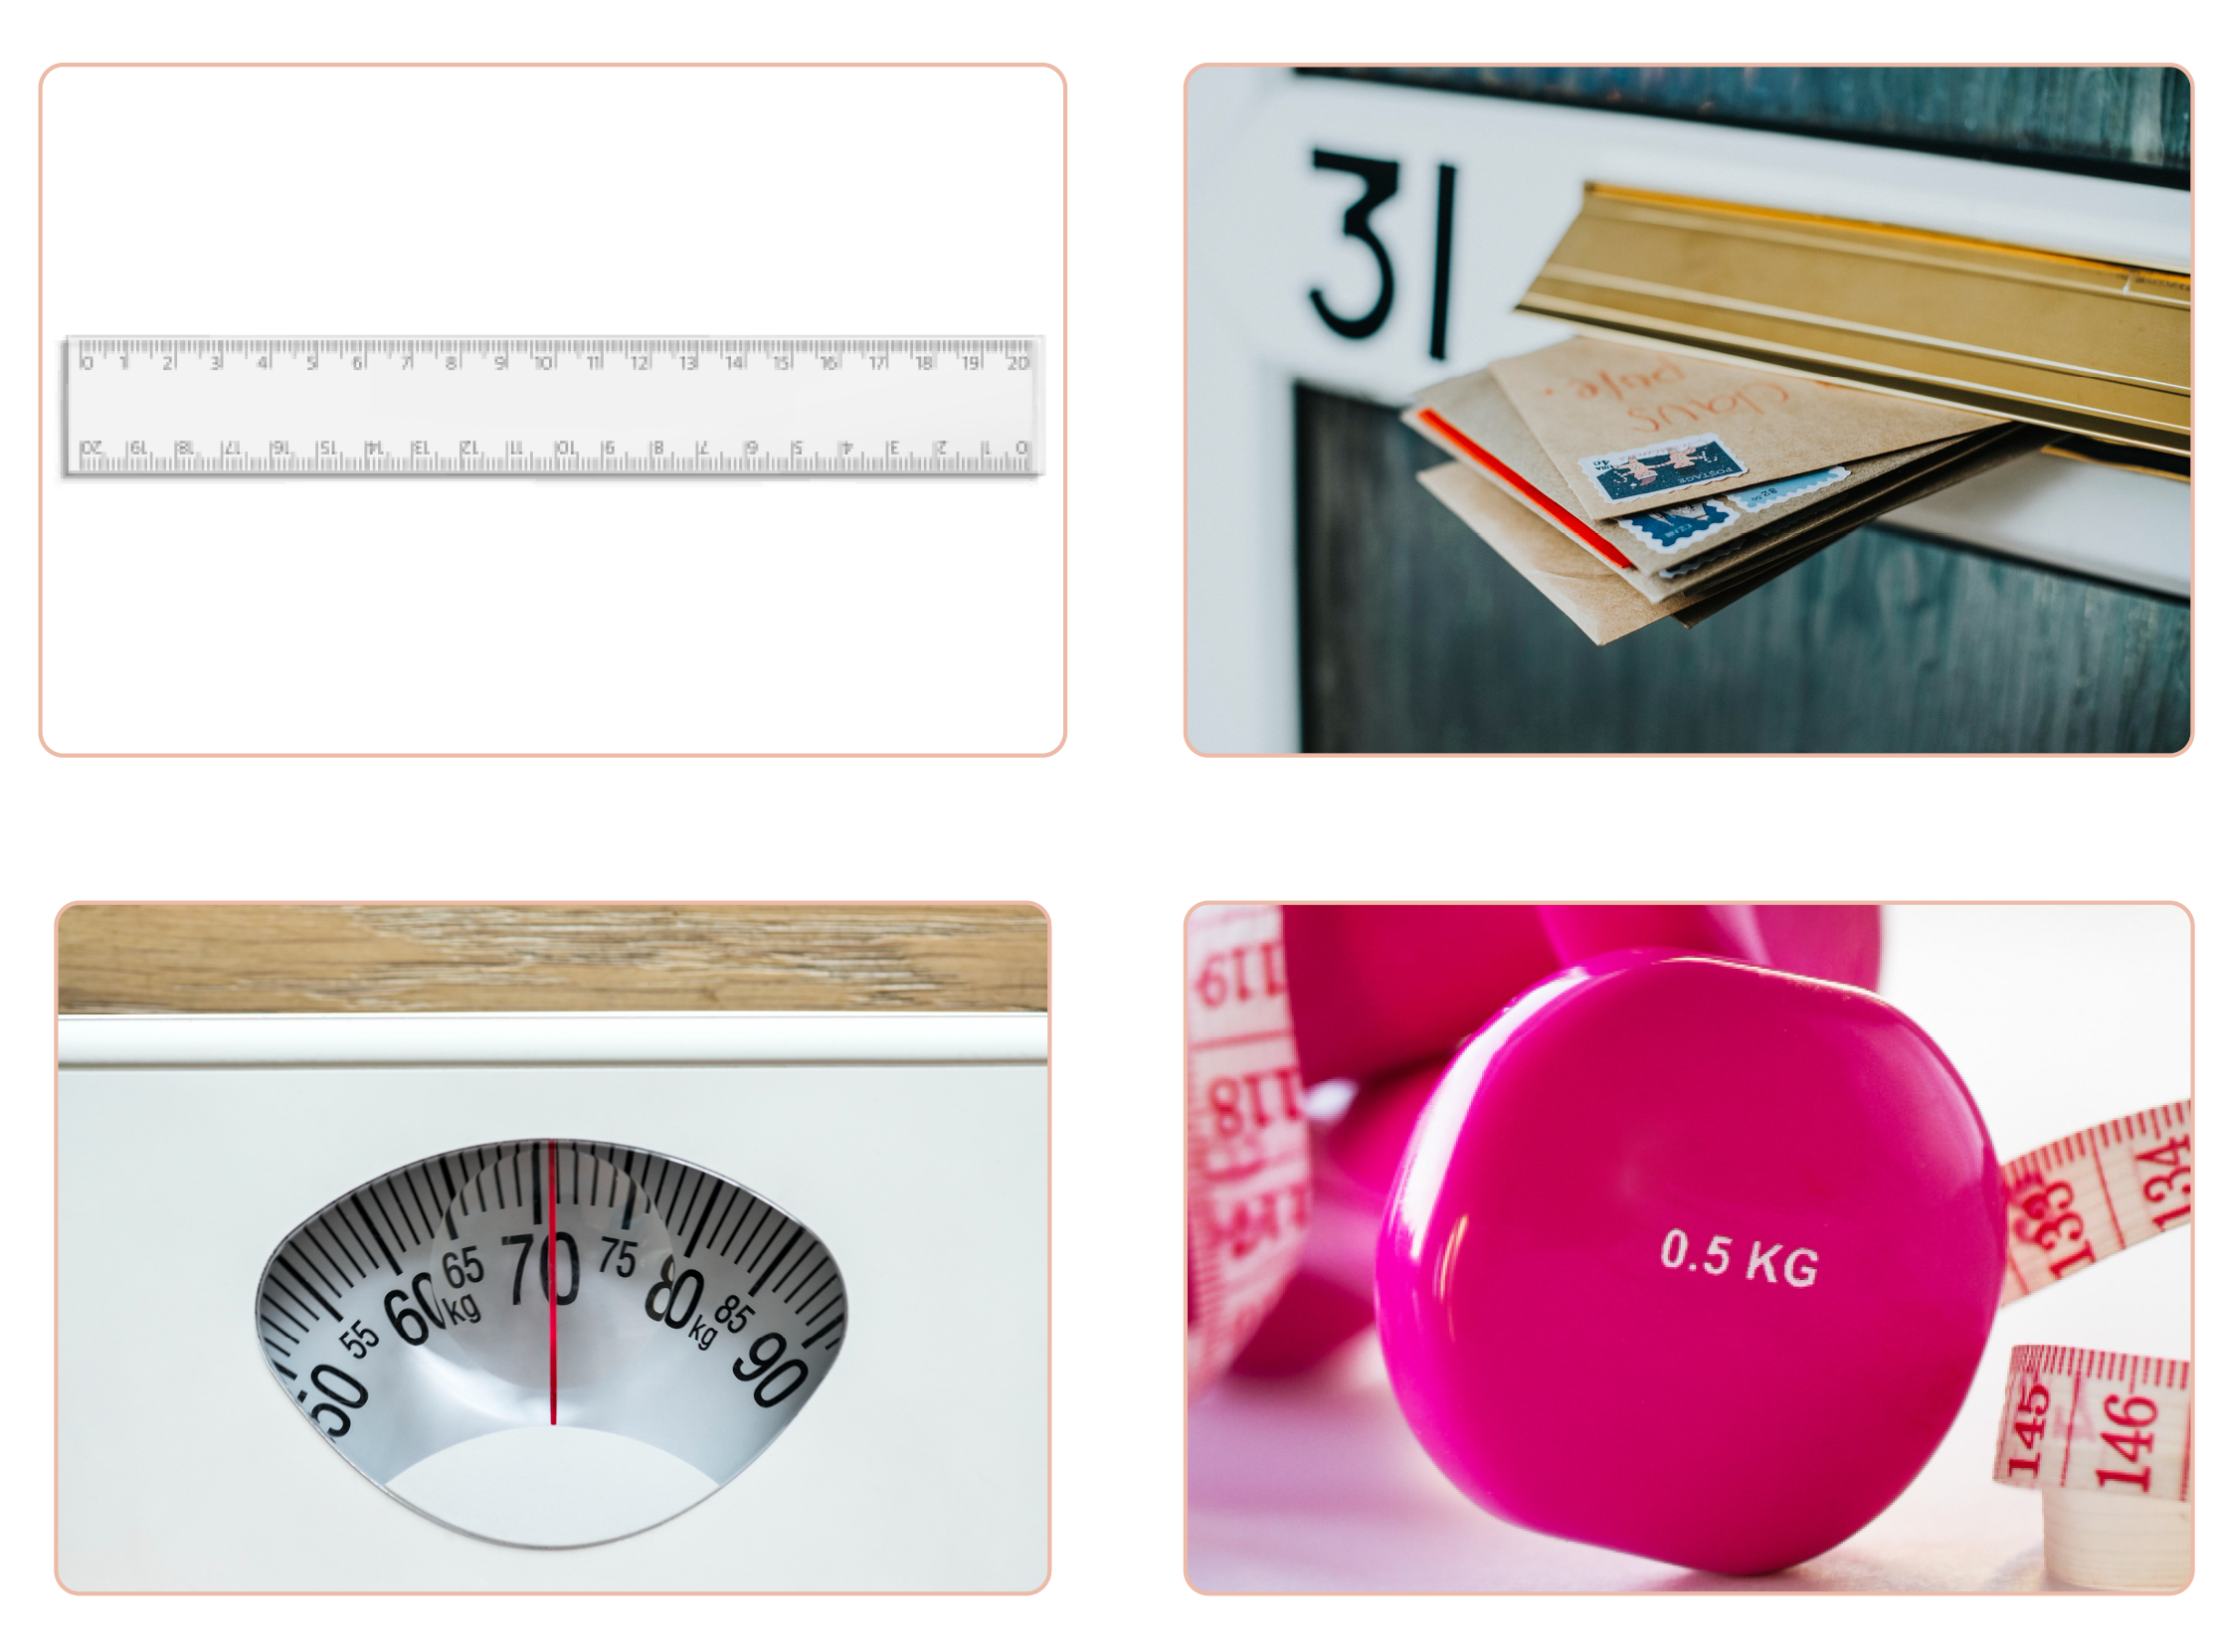
\includegraphics[width=.6\textwidth]{./media/SAEB_1ANO_MAT_FIGURA2.png}
\end{figure}

\rosa{O aluno deve circular a caixa de correio.}

\num{2} INDIQUE OS NÚMEROS DOS CARROS NA POSIÇÃO EM QUE CRUZARAM A LINHA DE CHEGADA.

%\textless{}Inserir o diagrama a seguir conforme modelo. Licenciar a figura: https://br.freepik.com/vetores-gratis/no-jogo-de-corrida-de-velocidade-o-jogador-do-driver-do-monstro-da-competicao-usou-o-carro-de-alta-velocidade-para-vencer-no-jogo\_16304604.htm\#query=carros\%20com\%20n\%C3\%BAmeros\&position=11\&from\_view=search\&track=ais.\textgreater{}

\begin{figure}[H]
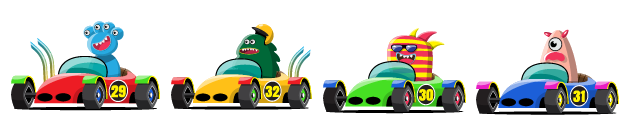
\includegraphics[width=\textwidth]{./media/SAEB_1ANO_MAT_FIGURA3.png}

\centering
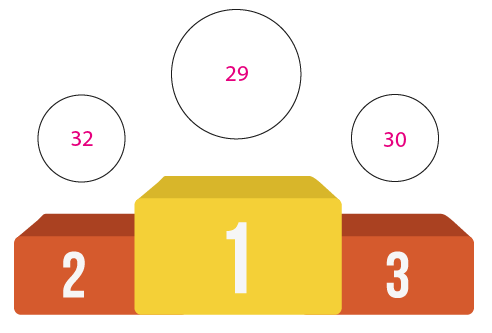
\includegraphics[width=.5\textwidth]{./media/SAEB_1ANO_MAT_FIGURA3a.png}
\end{figure}

\rosa{1-29; 2-32; 3-30.}

% \num{3} LIGUE OS NÚMEROS CORRETAMENTE.

% \begin{figure}[htpb!]
% \centering
% 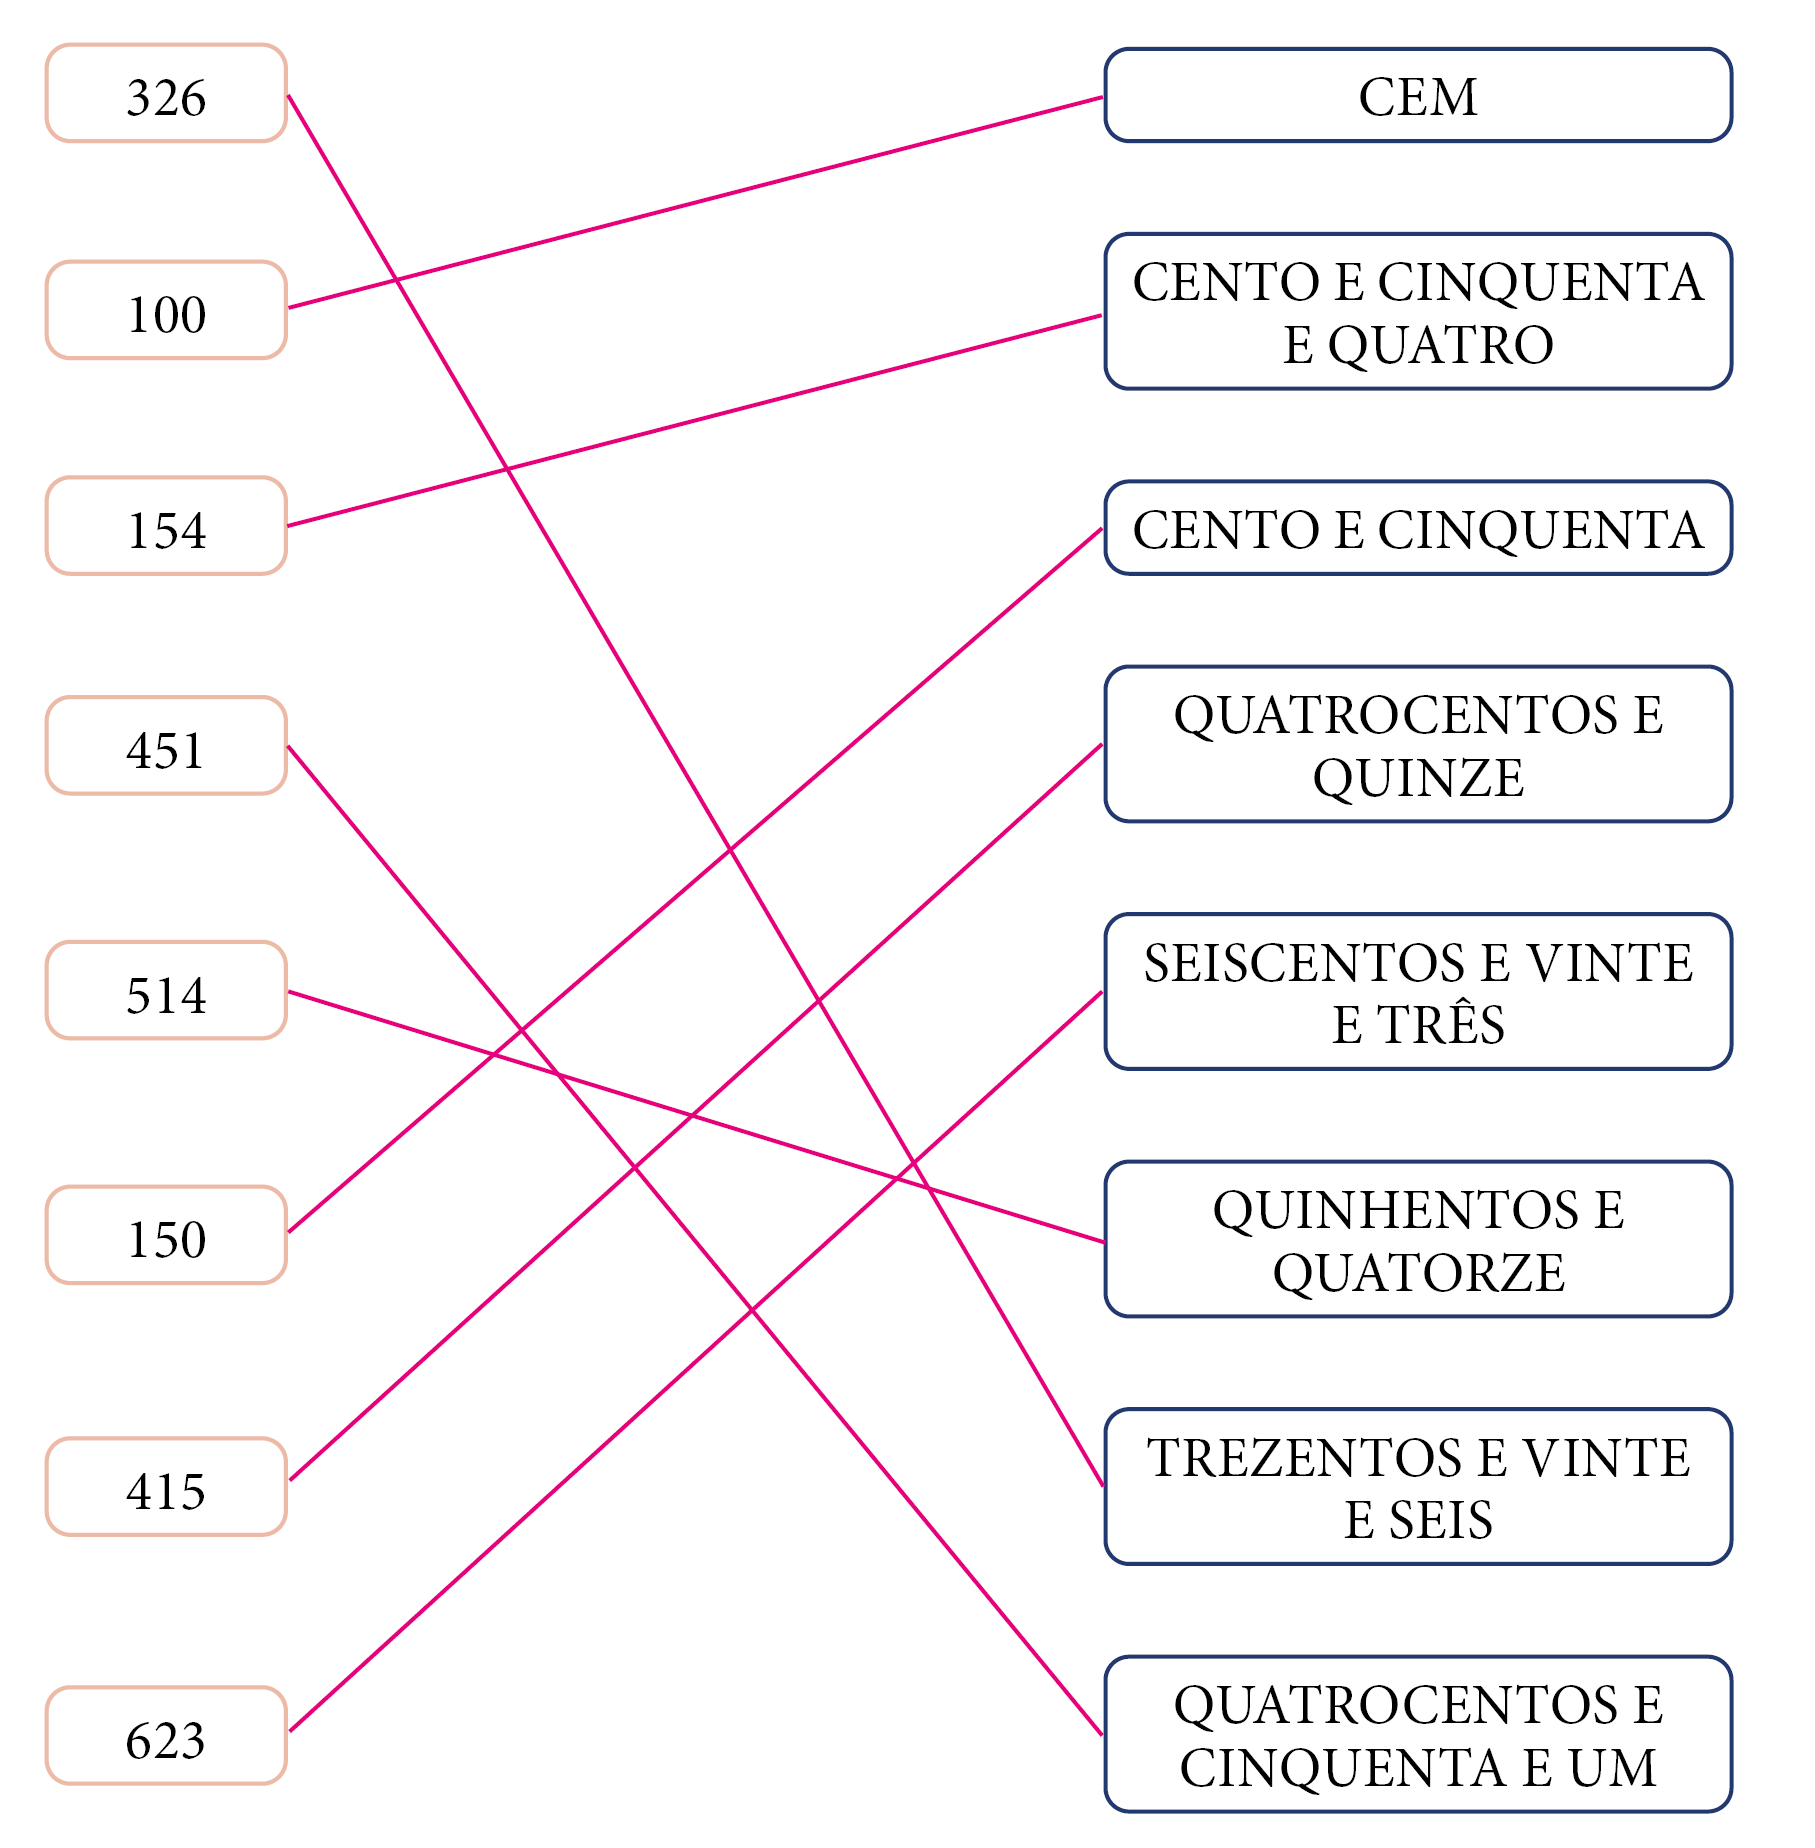
\includegraphics[width=\textwidth]{./media/SAEB_1ANO_MAT_FIGURA4.png}
% \end{figure}


\num{3} ALBERTO TEM UMA COLEÇÃO DE MINIATURAS. JÚNIOR TEM UMA COLEÇÃO DE BOLAS. QUAL DAS DUAS COLEÇÕES É A MAIOR?

%\textless{}Inserir figuras: https://br.freepik.com/vetores-gratis/time-de-futebol-ou-jogadores-de-time-de-futebol-em-fundo-branco\_10600572.htm\#query=cole\%C3\%A7\%C3\%A3o\%20de\%20figurinhas\&position=11\&from\_view=search\&track=ais; https://br.freepik.com/vetores-gratis/bolas-definir-ilustracao-vetorial\_4559016.htm\#query=cole\%C3\%A7\%C3\%A3o\%20de\%20bolas\&position=0\&from\_view=search\&track=ais. Não precisa traduzir os textos em inglês, pois eles não são necessários à resolução.\textgreater{}

\begin{figure}[htpb!]
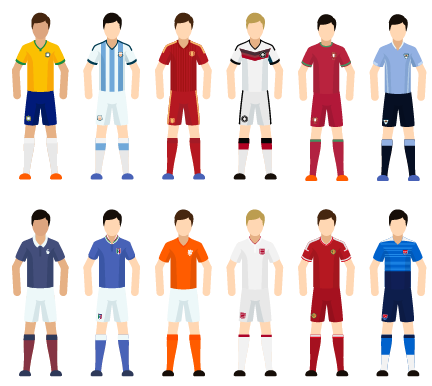
\includegraphics[width=.5\textwidth]{./media/SAEB_1ANO_MAT_FIGURA5.png}
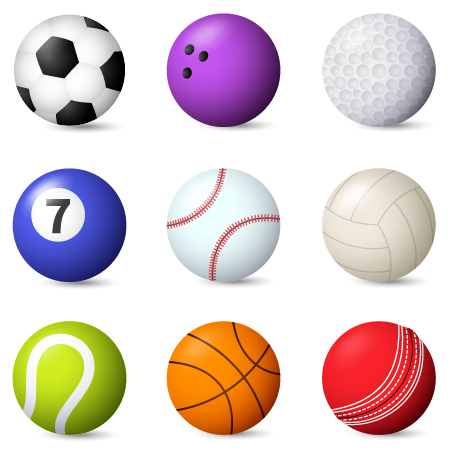
\includegraphics[width=.45\textwidth]{./media/SAEB_1ANO_MAT_FIGURA5a.png}
\end{figure}

\reduline{O aluno deve contar as duas coleções e perceber que a coleção de camisas de Alberto é maior, pois tem mais unidades do que a coleção de Júnior.\hfill}

\num{4} AINDA SOBRE A SITUAÇÃO APRESENTADA NA ATIVIDADE ANTERIOR, RESPONDA AO QUE SE PERGUNTA A SEGUIR.

\begin{escolha}
\item
  QUANTAS MINIATURAS ALBERTO TEM?\\
\reduline{12 camisas.\hfill}

\item
  QUANTAS BOLAS JÚNIOR TEM?\\
\reduline{9 bolas.\hfill}

\item
  QUANTOS ITENS ALBERTO TEM EM SUA COLEÇÃO A MAIS QUE OS ITENS QUE JÚNIOR TEM EM SUA COLEÇÃO?\\
  \reduline{3 itens.\hfill}
\end{escolha}


\num{5} CIRCULE O CONJUNTO DE DADOS COM O MAIOR RESULTADO. LEMBRE-SE DE OLHAR PARA A FACE DO DADO VOLTADA PARA CIMA.

%\textless{} Inserir um quadro com as imagens conforme o modelo a seguir. https://br.freepik.com/vetores-gratis/dados-isometricos-cubos-de-jogo-pretos-variantes-isolados-no-fundo-branco-coleta-de-todas-as-voltas-possiveis\_13090027.htm\#query=dice\&position=1\&from\_view=search\&track=sph.\textgreater{}

\begin{figure}[htpb!]
\centering
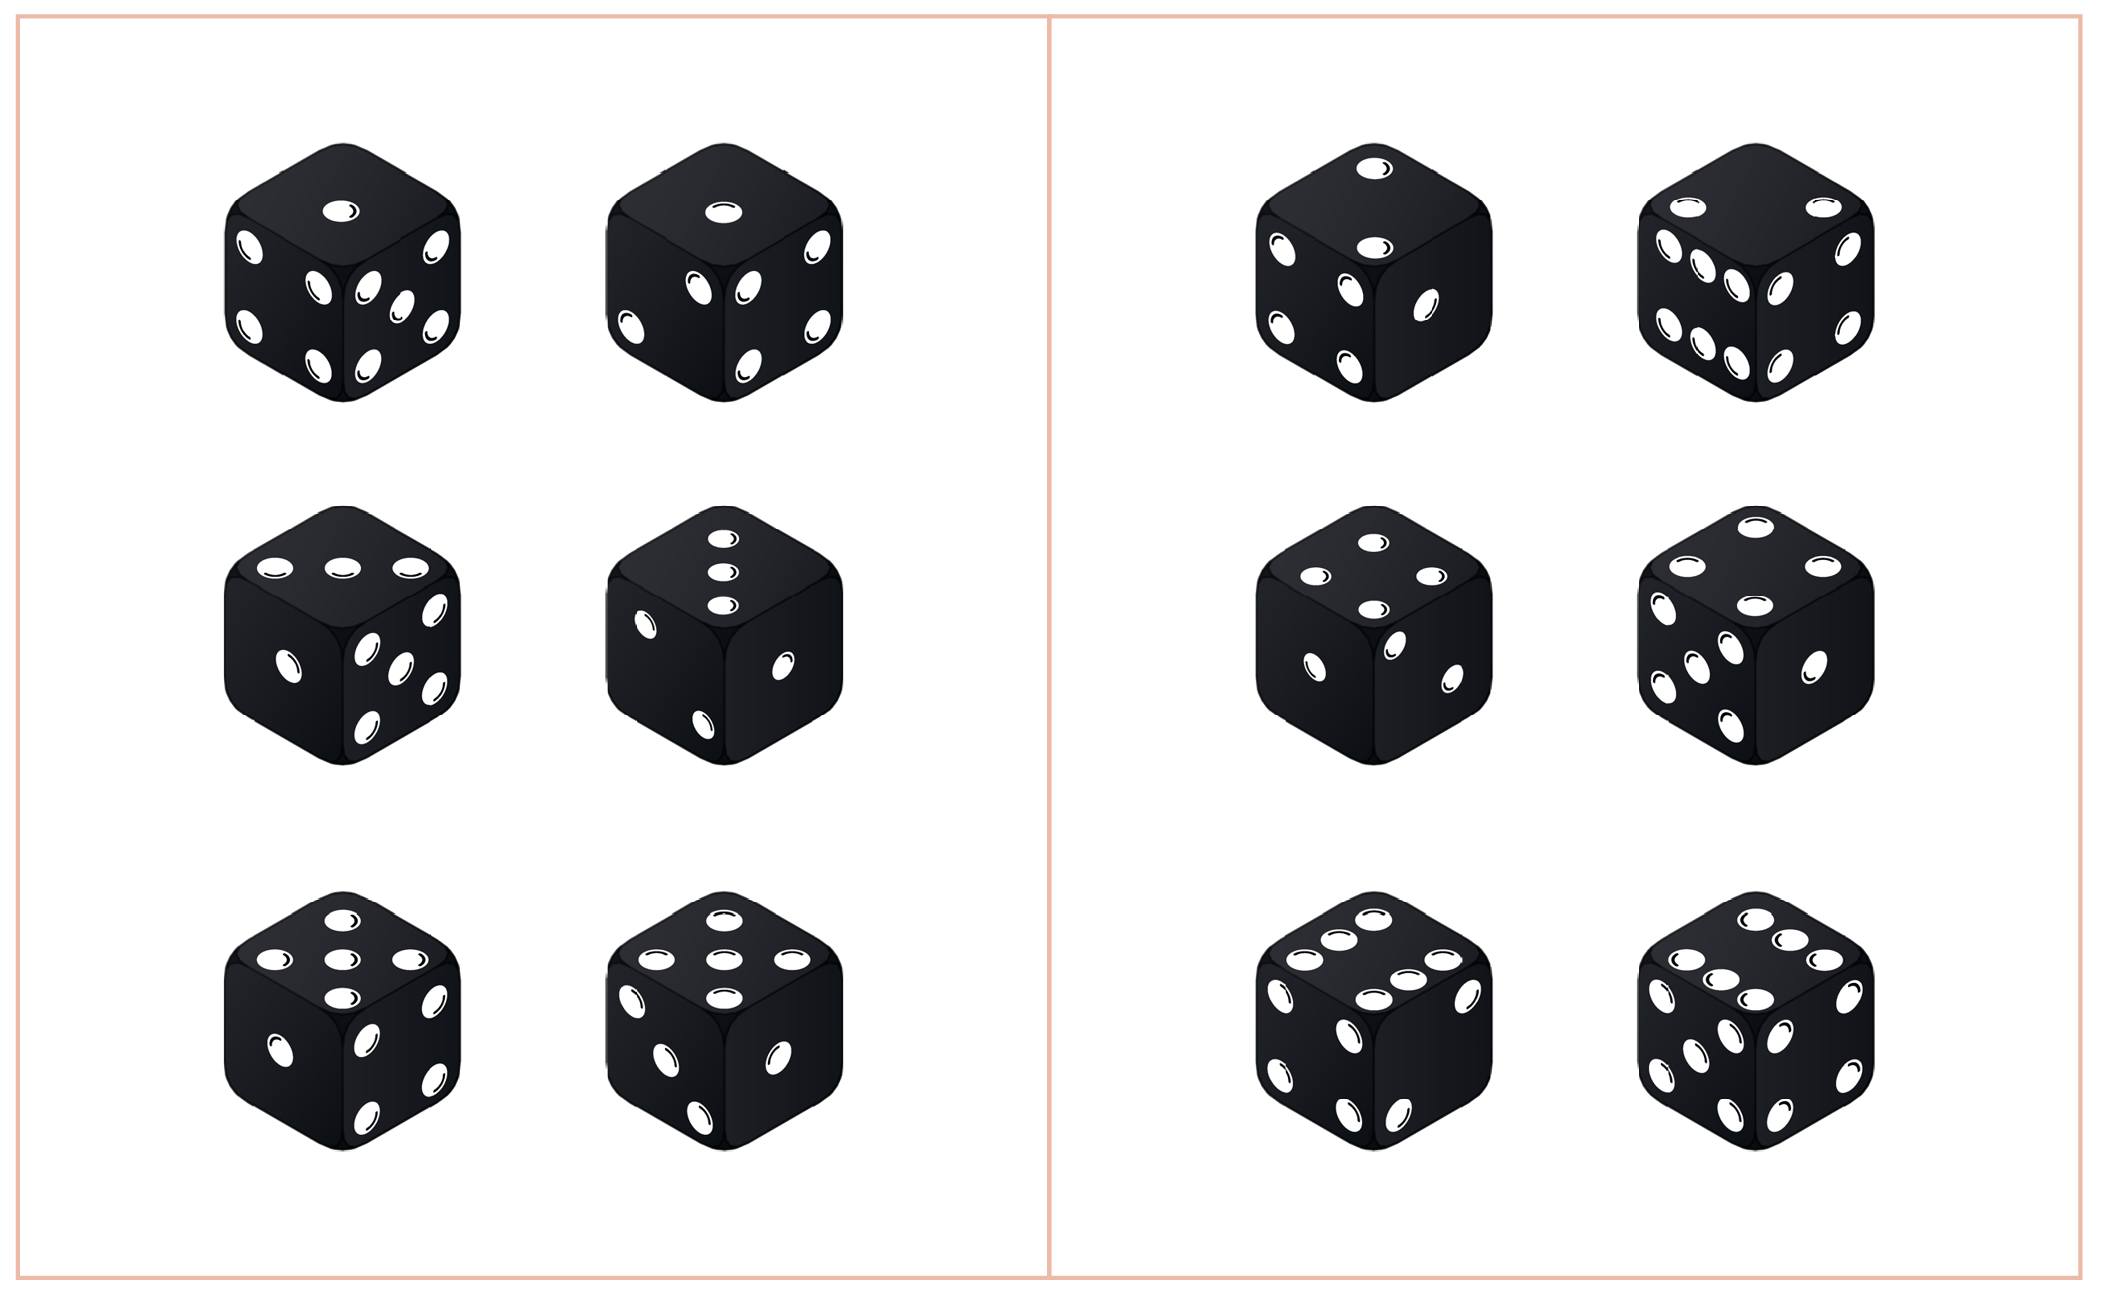
\includegraphics[width=.6\textwidth]{./media/SAEB_1ANO_MAT_FIGURA6.png}
\end{figure}

\rosa{A imagem a ser circulada é a da direita.}

\num{6} AINDA SOBRE OS DADOS, FAÇA O QUE SE PEDE A SEGUIR.

\begin{figure}[htpb!]
\centering
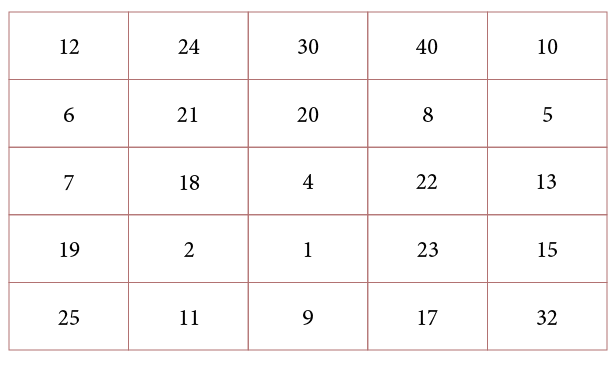
\includegraphics[width=.7\textwidth]{./media/SAEB_1ANO_MAT_FIGURA7.png}
\end{figure}

\begin{escolha}[itemsep=-5pt]
\item PINTE DE AZUL O NÚMERO DA SOMA DOS DADOS DA DIREITA.

\item PINTE DE VERDE O NÚMERO DA SOMA DOS DADOS DA ESQUERDA.

\item PINTE DE AMARELO A DIFERENÇA ENTRE AS SOMAS.
\end{escolha}

\rosa{Número 22: azul. Número 18: verde. Número 4: amarelo.}

\num{7} ESCREVA OS SEGUINTES NÚMEROS EM ORDEM CRESCENTE.

\begin{escolha}
\item 516 -- 645 -- 215 -- 326 - 789
\reduline{215 - 326 -- 516 -- 645 -- 789\hfill}


\item 132 -- 165 -- 112 -- 115 -- 100
\reduline{100 -- 112 -- 115 -- 132 -- 165\hfill}


\item 325 -- 854 -- 127 -- 974 -- 546
\reduline{127 -- 325 -- 546 -- 854 -- 974\hfill}


\item 415 -- 418 -- 411 -- 410 -- 417
\reduline{410 -- 411 -- 415 -- 417 -- 418\hfill}

% \item 798 -- 987 -- 879 -- 897 -- 978
% \reduline{798 -- 879 -- 897 -- 978 -- 987\hfill}

% \item 623 -- 236 -- 362 -- 326 -- 263
% \reduline{236 -- 263 -- 326 -- 362 -- 623\hfill}
\end{escolha}


\num{8} ESCREVA OS SEGUINTES NÚMEROS EM ORDEM DECRESCENTE.

\begin{escolha}
\item 564 -- 456 -- 546 -- 645 -- 465
\reduline{645 -- 564 -- 546 -- 465 -- 456\hfill}

\item 138 -- 831 -- 318 -- 183 -- 813
\reduline{831 -- 813 -- 318 -- 183 -- 138\hfill}

\item 715 -- 517 -- 751 -- 571 -- 175
\reduline{751 -- 715 -- 571 -- 517 -- 175\hfill}

\item 833 -- 383 -- 838 -- 338 -- 388
\reduline{838 -- 833 -- 388 -- 383 -- 338\hfill}

% \item 717 -- 177 -171 -- 117 -- 771
% \reduline{771 -- 717 -- 177 -- 171 -- 117\hfill}

% \item 100 -- 200 -- 300 - 400 -- 500
% \reduline{500 -- 400 -- 300 -- 200 -- 100\hfill}
\end{escolha}

\num{9} JERÔNIMO MORA NA CASA 328 DA RUA SANTOS, EM SUA
CIDADE. LIGUE CORRETAMENTE OS ALGARISMOS DO NÚMERO DA CASA,
QUE ESTÃO NA COLUNA DA ESQUERDA, ÀS ORDENS CORRESPONDENTES,
QUE ESTÃO NA COLUNA DA DIREITA.

\begin{multicols}{2}
3

2

8

\columnbreak

Dezenas

Centenas

Unidades
\end{multicols}

\rosa{3: centenas. 2: dezenas. 8: unidades.}

% \num{9} PINTE OS QUADRADOS COM A COR DA ORDEM CORRESPONDENTE.

% %\textless{}Criar um afigura conforme o modelo a seguir.\textgreater{}

% \begin{minipage}{.8\textwidth}
% 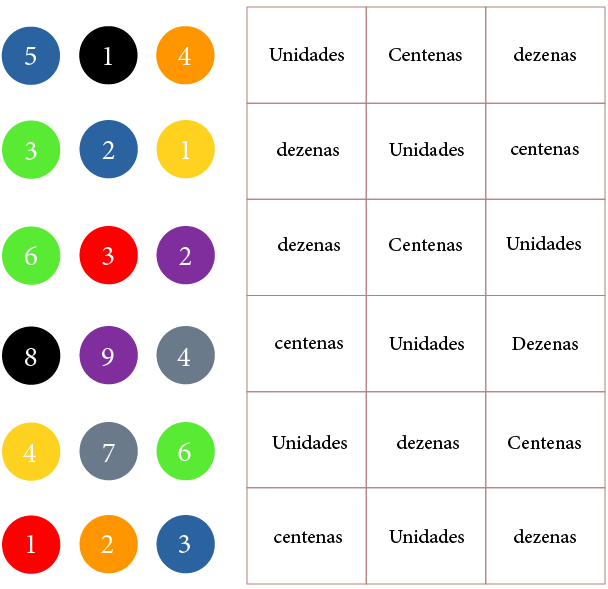
\includegraphics[width=\textwidth]{./media/SAEB_1ANO_MAT_FIGURA11.png}
% \end{minipage}\hspace*{-1cm}
% \sidetext{
% \begin{longtable}[]{@{}lll@{}}
% \toprule
% laranja & azul & Preto\tabularnewline
% azul & amarelo & Verde\tabularnewline
% vermelho & verde & Roxo\tabularnewline
% preto & cinza & Roxo\tabularnewline
% verde & cinza & Amarelo\tabularnewline
% vermelho & azul & Laranja\tabularnewline
% \bottomrule
% \end{longtable}
% }

\num{10} OS TRÊS COMPETIDORES REPRESENTADOS ESTÃO NO PÓDIO. ELES TÊM OS NOMES ESCRITOS NA CAMISETA. DESCUBRA QUAL É A PONTUAÇÃO DE CADA UM DELES E ESCREVA SEUS NOMES NA TABELA.

%\textless{}Inserir a figura de referência: https://br.freepik.com/vetores-gratis/podio-esportes\_1040693.htm\#query=podium\%20com\%20competidores\&position=1\&from\_view=search\&track=ais. Acrescente os nomes dos competidores, conforme o modelo a seguir.\textgreater{}

\begin{figure}[H]
\centering
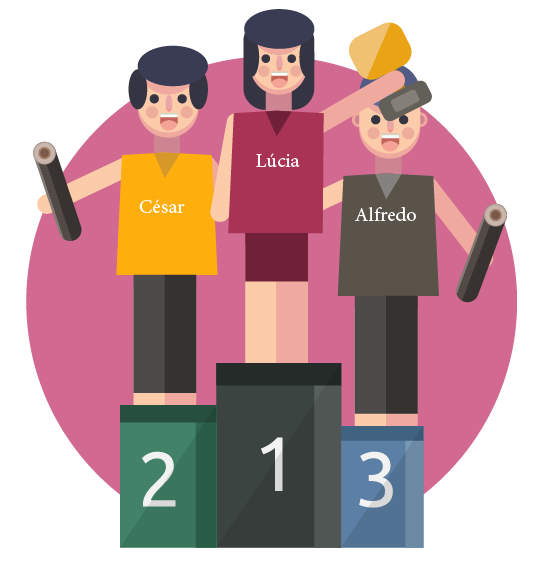
\includegraphics[width=.9\textwidth]{./media/SAEB_1ANO_MAT_FIGURA13.png}
\end{figure}

\begin{longtable}[]{@{}ll@{}}
\toprule
\textbf{PONTUAÇÃO} & \textbf{NOME}\tabularnewline
1.000 PONTOS & \rosa{ALFREDO FOI O TERCEIRO COLOCADO.}\tabularnewline
1.005 PONTOS & \rosa{LÚCIA FOI A PRIMEIRA COLOCADA.}\tabularnewline
1.0004 PONTOS & \rosa{CÉSAR FOI O SEGUNDO COLOCADO.}\tabularnewline
\bottomrule
\end{longtable}

%\coment{É importante que os alunos compreendam que o primeiro colocado deve ter feito a maior quantidade de pontos, e assim por diante.}

 
\num{11} A RETA NUMERADA A SEGUIR REPRESENTA UMA RUA QUALQUER DE UM BAIRRO. LIGUE AS CASAS ÀS SUAS RESPECTIVAS POSIÇÕES CONFORME O NÚMERO.

%\textless{}Criar uma reta numérica conforme o modelo a seguir. Depois colocar a figura de referência: https://br.freepik.com/vetores-gratis/pacote-de-belas-fachadas-de-casas-desenhadas-a-mao\_1198631.htm\#page=2\&query=casas\%20coloridas\&position=11\&from\_view=search\&track=ais com os respectivos números conforme o modelo.

\begin{figure}[htpb!]
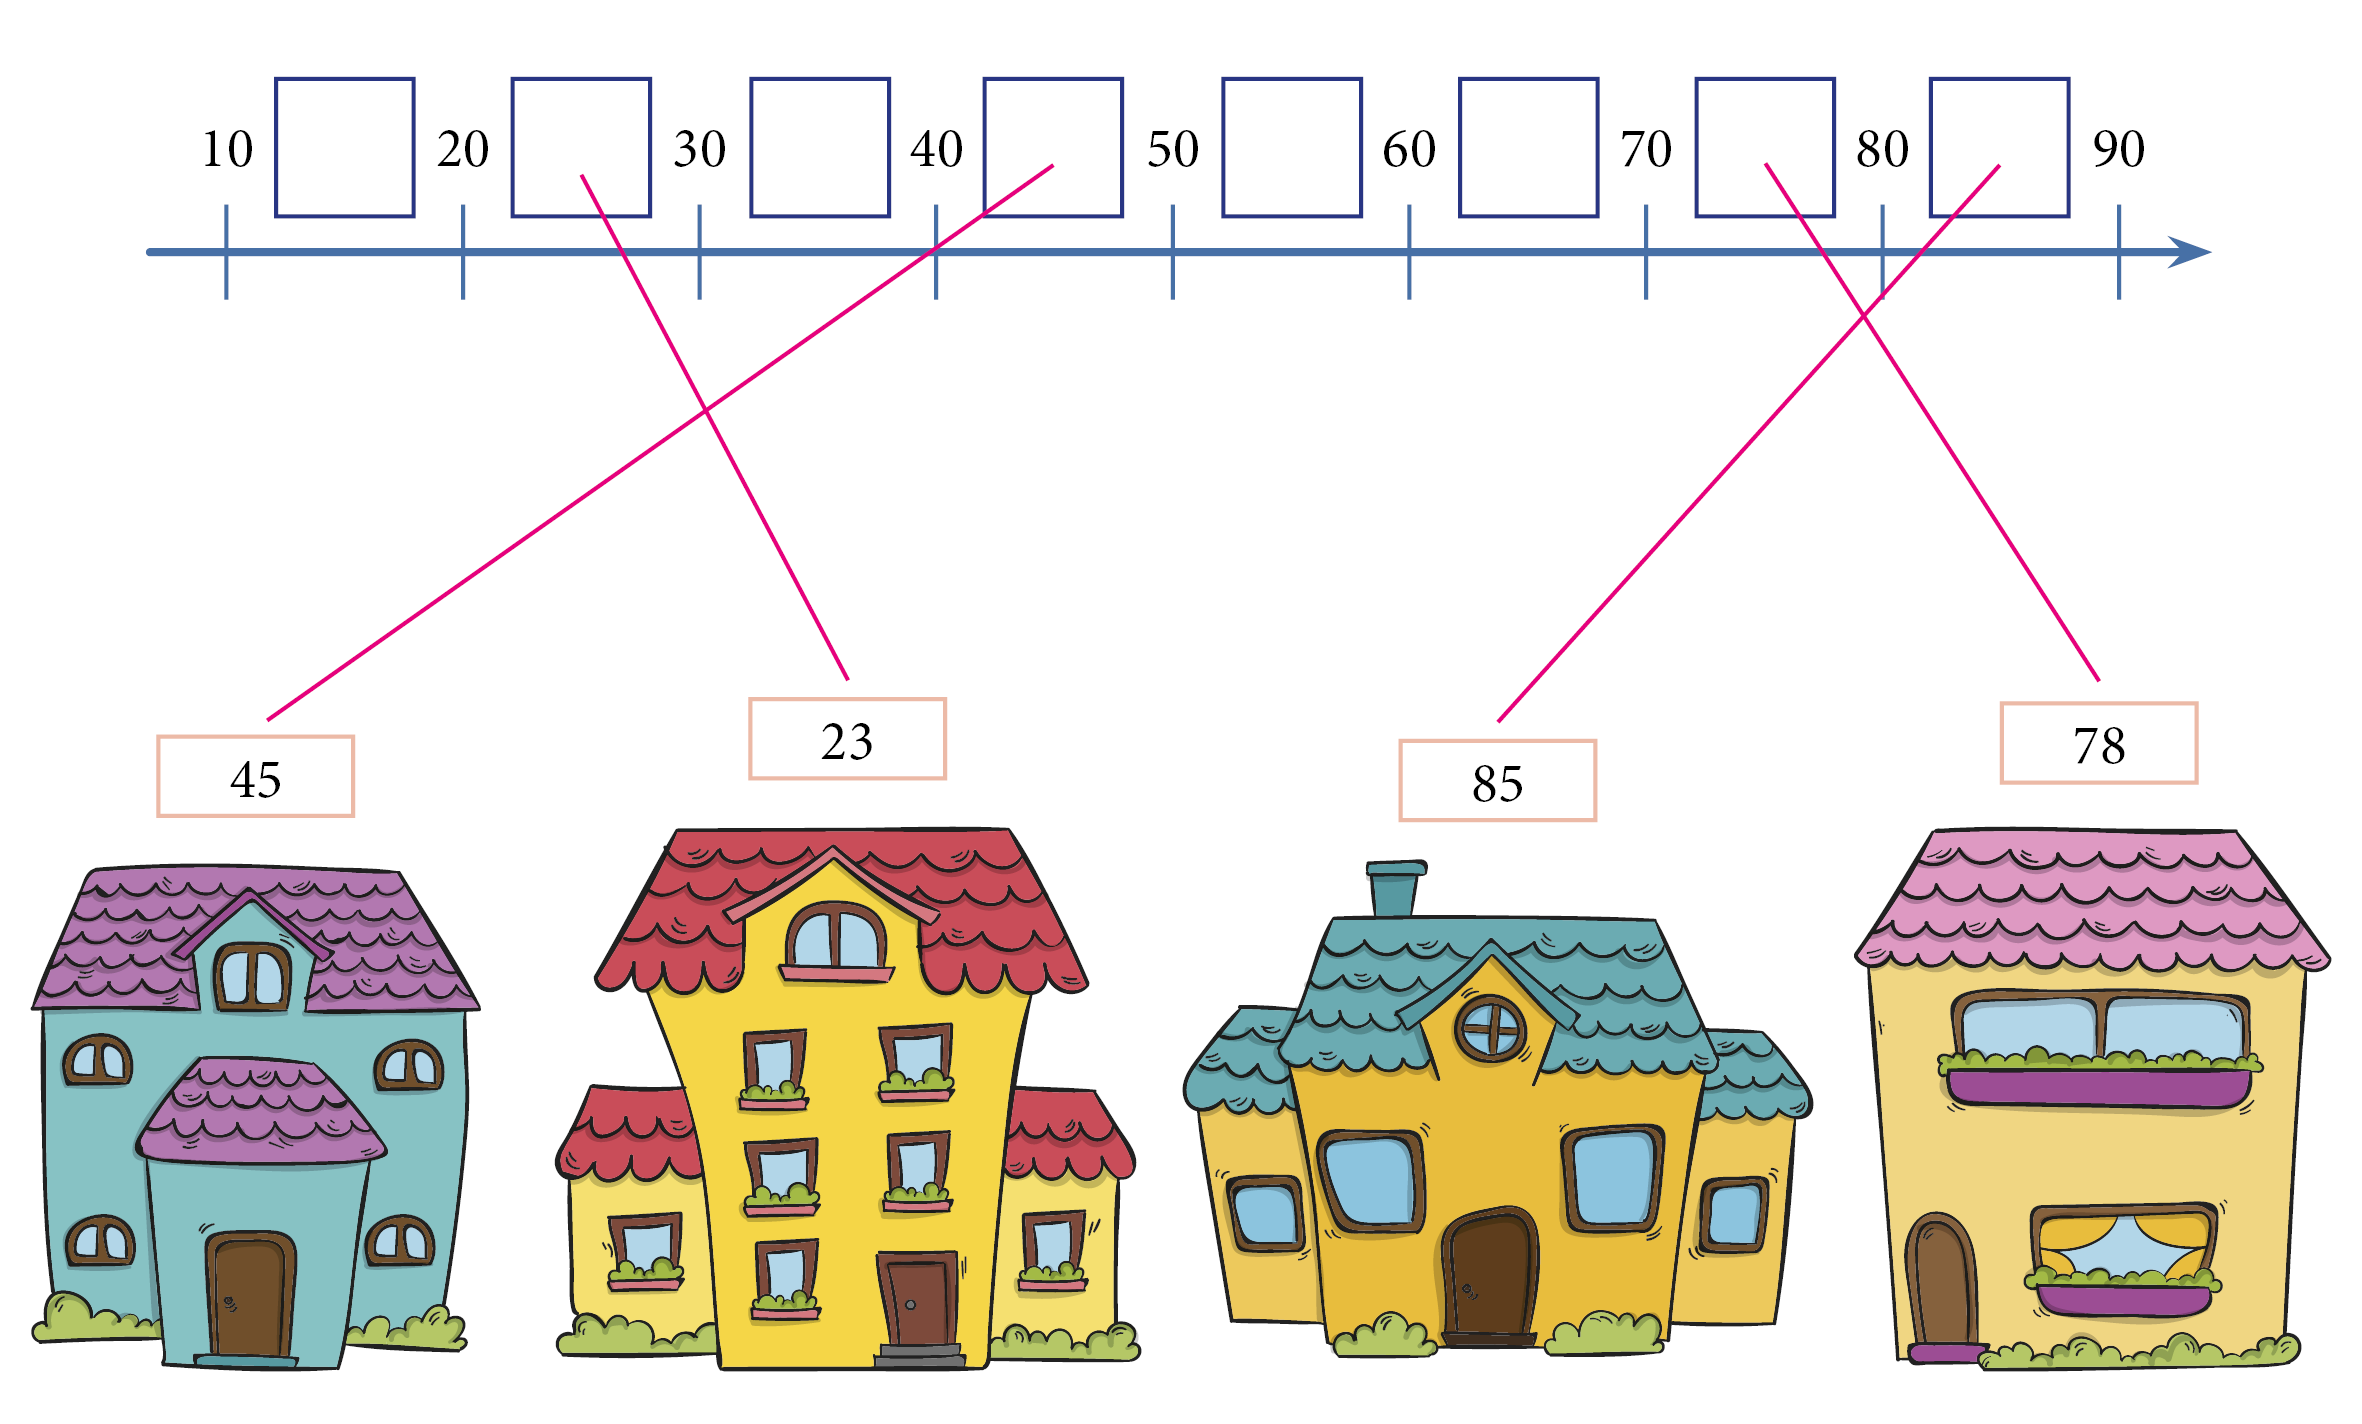
\includegraphics[width=\textwidth]{./media/SAEB_1ANO_MAT_FIGURA14.png}
\end{figure}

% \num{12} ESCREVA OS NÚMEROS A SEGUIR COM ALGARISMOS.

% \begin{center}
% \Large
% \begin{tabular}{|l|l|}
% \hline
% SEISCENTOS E DEZENOVE & \rosa{619} \\ \hline
% OITOCENTOS E TRINTA E SETE & \rosa{837} \\ \hline
% NOVECENTOS E QUARENTA E UM & \rosa{941} \\ \hline
% CENTO E DOIS & \rosa{102} \\ \hline
% CENTO E TRINTA E OITO & \rosa{138} \\ \hline
% DUZENTOS E VINTE E CINCO & \rosa{225} \\ \hline
% TREZENTOS E OITENTA E QUATRO & \rosa{384} \\ \hline
% QUATROCENTOS E QUINZE & \rosa{415} \\ \hline
% QUINHENTOS E SETENTA E SETE & \rosa{577} \\ \hline
% SETECENTOS E DEZESSEIS & \rosa{716} \\ \hline
% CENTO E CINQUENTA E TRÊS & \rosa{153} \\ \hline
% \end{tabular}
% \end{center}

\section*{TREINO}

\num{1} NA CARTEIRINHA DA ESCOLA DE JÚLIA, APARECE SUA FOTO, SEU NOME E O NÚMERO DO
REGISTRO DE MATRÍCULA. NO CASO DE JÚLIA, ESSE NÚMERO É O 363. ESSE NÚMERO INDICA

\begin{escolha}
\item
  QUANTIDADE.
\item
  ORDEM.
\item
  MEDIDA.
\item
  IDENTIFICAÇÃO.
\end{escolha}

\num{2} NA IMAGEM, MOSTRAM-SE QUATRO COLEÇÕES DE AMIGOS QUE GOSTAM DE COLECIONAR
BOLINHAS DE GUDE.

\begin{figure}[H]
\centering
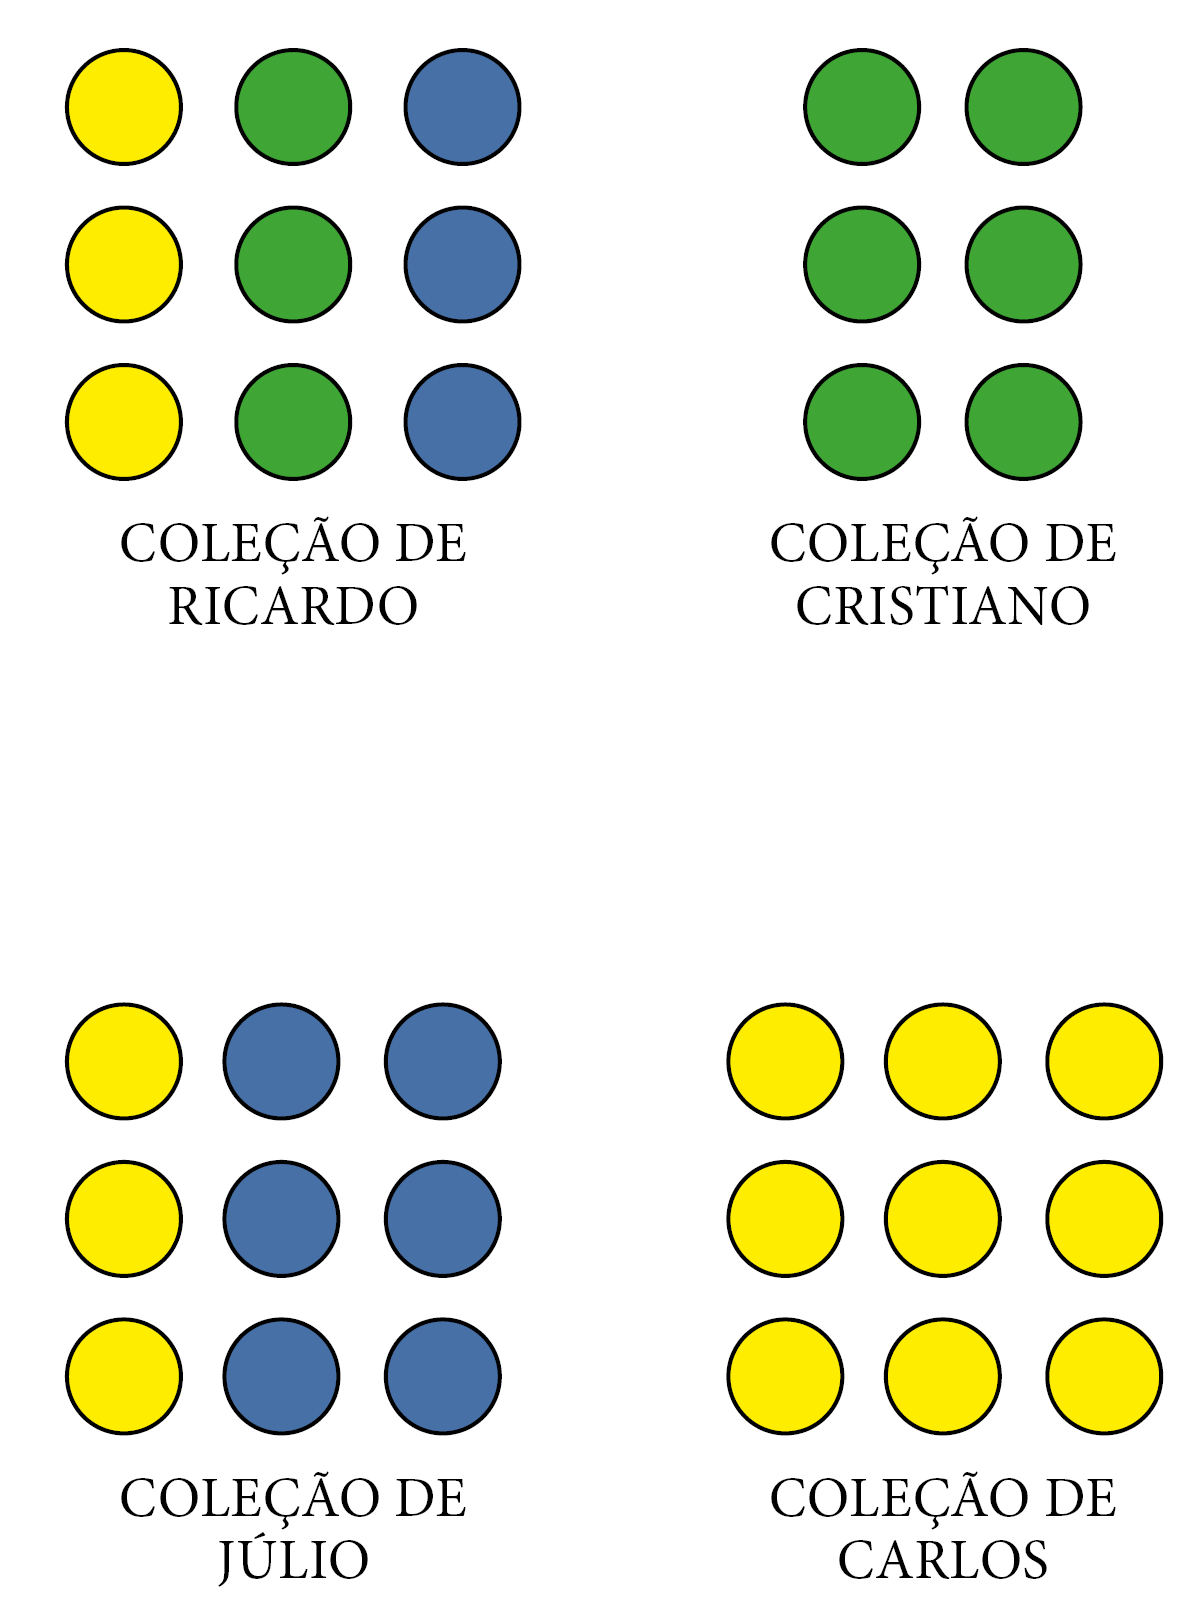
\includegraphics[width=.5\textwidth]{./media/SAEB_1ANO_MAT_FIGURA16.png}
\end{figure}

\noindent{}QUEM É O DONO DA COLEÇÃO QUE TEM A MAIOR QUANTIDADE DE BOLINHAS DE UMA ÚNICA COR?

\begin{escolha}
\item
  CARLOS.
\item
  CRISTIANO.
\item
  JÚLIO.
\item
  RICARDO.
\end{escolha}

\num{3} ENTRE 0 E 100, QUANTOS NÚMEROS TERMINAM COM O NÚMERO ZERO NA ORDEM DAS UNIDADES?

\begin{multicols}{2}
\begin{escolha}
\item
  1.
\item
  9.
\item
  10.
\item
  11.
\end{escolha}
\end{multicols}

\chapter{JUNTAR OU TIRAR?}
\markboth{Módulo 2}{}

%\coment{Neste módulo, vamos desenvolver a habilidade de desenvolvimento de cálculos, tanto no sentido de escolher a melhor estratégia, quanto no sentido de resolver o problema. Faremos essa abordagem de forma abstrata, mas também de forma contextualizada, com o fim de desenvolver nos alunos a motivação para resolverem problemas reais.}

\section*{HABILIDADES DO SAEB}

\begin{itemize}
\item \uppercase{Calcular o resultado de adições e subtrações, envolvendo número
naturais de até 3 ordens.}

\item \uppercase{Compor ou decompor números naturais de até 3 ordens por meio de
diferentes adições.}

\item \uppercase{Resolver problemas de adição ou de subtração, envolvendo números
naturais de até 3 ordens, com os significados de juntar, acrescentar,
separar ou retirar.}
\end{itemize}

\subsection{HABILIDADES DA BNCC}

\begin{itemize}
\item EF01MA07, EF01MA08.
\end{itemize}

\conteudo{
MÁRCIA GANHOU DO PAI DUAS NOTAS DE DEZ REAIS E DECIDIU QUE
QUERIA COMPRAR UM BRINQUEDO QUE CUSTAVA QUINZE REAIS. MÁRCIA PERCEBEU
QUE TINHA UM PROBLEMA: PARA SABER SE ELA TERIA CONDIÇÕES DE COMPRAR
AQUELE BRINQUEDO, ELA TERIA DE DESCOBRIR QUANTO DINHEIRO TINHA. SEU PAI
RESOLVEU AJUDAR. ELE PEGOU A QUANTIDADE DE PALITOS EQUIVALENTE AO VALOR DAS
NOTAS. OBSERVE:

%\textless{}Criar uma ilustração com duas carreiras de 10 palitos alinhadas a uma cédula de 10 reais, conforme o modelo a seguir. https://www.istockphoto.com/br/foto/dez-real-brasileiro-gm181402095-26926813?utm\_campaign=srp\_photos\_inline\&utm\_content=https\%3A\%2F\%2Fwww.pexels.com\%2Fprocurar\%2F10\%2520reais\%2F\&utm\_medium=affiliate\&utm\_source=pexels\&utm\_term=10+reais https://br.freepik.com/fotos-premium/uma-partida-com-cabeca-verde-em-um-fundo-branco\_31512045.htm\#page=3\&query=palito\%20de\%20f\%C3\%B3sforo\&position=18\&from\_view=search\&track=ais\textgreater{}

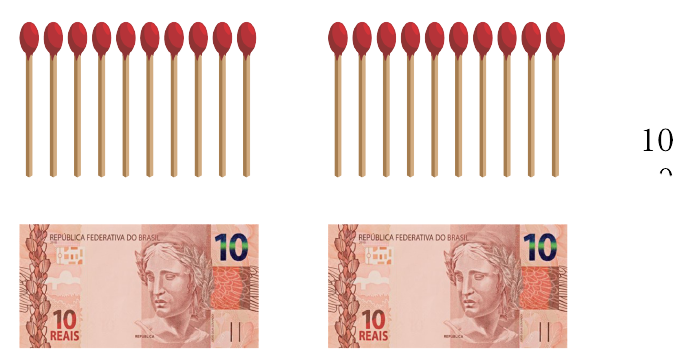
\includegraphics[width=\textwidth]{./media/SAEB_1ANO_MAT_FIGURA17.png}

MÁRCIA CONTOU OS PALITOS E PERCEBEU QUE TINHA 20 REAIS. AGORA, ELA
PRECISAVA SABER SE ESSES 20 REAIS SERIAM SUFICIENTES PARA COMPRAR O
BRINQUEDO. A PRÓPRIA MÁRCIA PEGOU MAIS QUINZE PALITINHOS E OS ALINHOU DA
SEGUINTE FORMA:

%\textless{}Criar uma figura com duas linhas de palito alinhados. Na primeira linha 20 e na segunda linha 15. Colocar a operação ao lado, conforme modelo a seguir.\textgreater{}

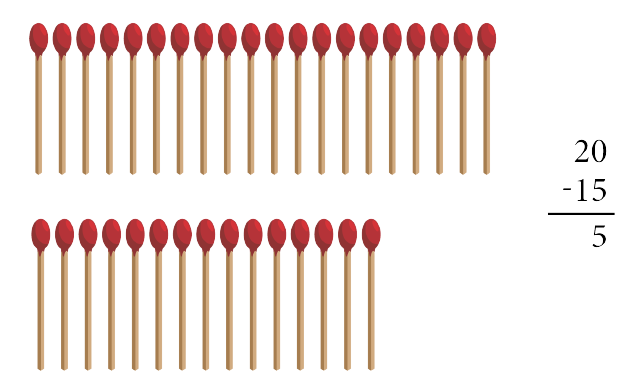
\includegraphics[width=\textwidth]{./media/SAEB_1ANO_MAT_FIGURA18.png}

MÁRCIA FICOU MUITO FELIZ AO PERCEBER QUE PODERIA COMPRAR SEU BRINQUEDO.
E AINDA LHE SOBRARIAM CINCO REAIS PARA COMPRAR UM LANCHE.
}

\section*{ATIVIDADES}

\num{1} PINTE O FOGUETE COM AS CORES CORRETAS. DESCUBRA AS CORES RESOLVENDO AS
ADIÇÕES.

%\textless{}Inserir um quadro conforme o modelo a seguir. https://br.freepik.com/vetores-premium/foguete-de-desenho-bonito-de-cor-planilha-para criancas\_22159996.htm\#page=6\&query=para\%20colorir\%20foguete\&position=7\&from\_view=search\&track=ais.\textgreater{}

\begin{figure}[htpb!]
\centering
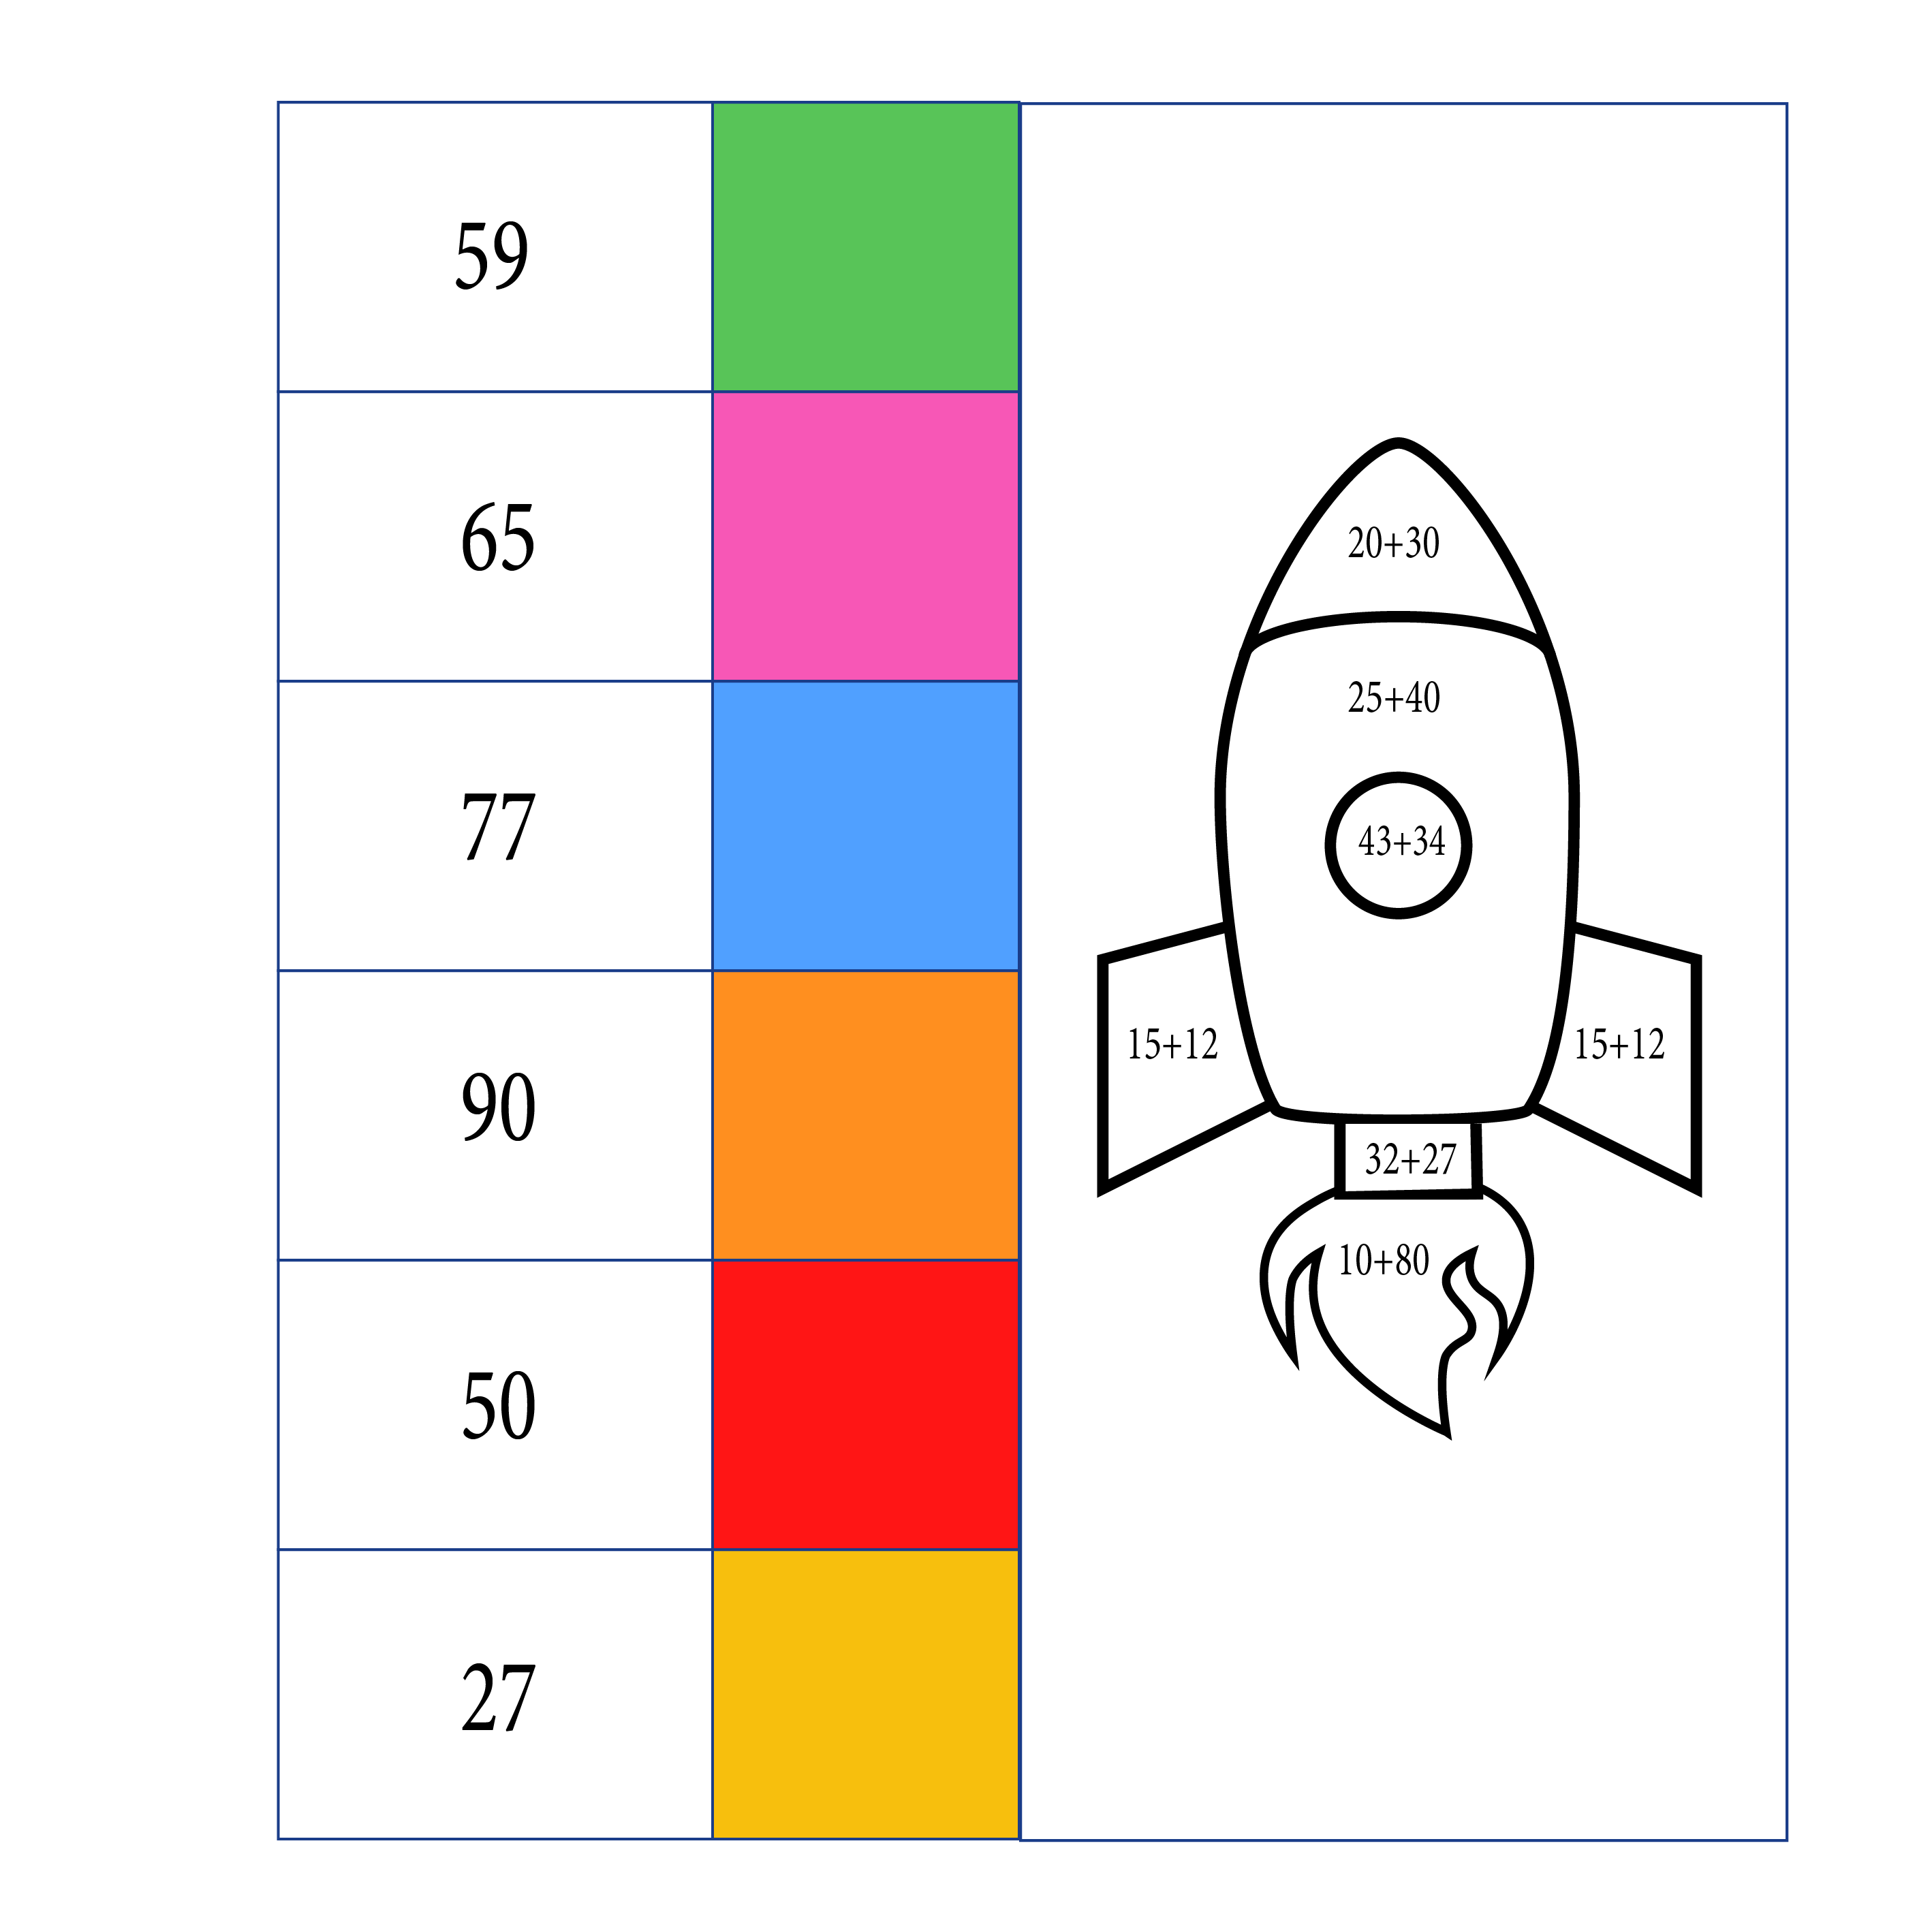
\includegraphics[width=\textwidth]{./media/SAEB_1ANO_MAT_FIGURA19.png}
\end{figure}

%\coment{Oriente os alunos a resolverem as adições primeiro, antes de começarem a pintar o foguete. No quadro à esquerda, temos as resoluções das adições. Nele, o aluno deve pintar o pedaço do foguete com a cor correspondente.}

\rosa{20 + 30 = vermelho; 25 + 40 = rosa; 43 + 34 = azul; 15 + 12 = amarelo;
32 + 27 = verde; 10 + 80 = laranja.}

%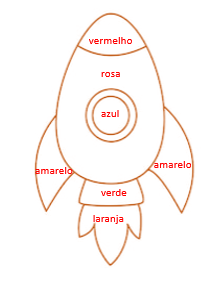
\includegraphics[width=1.43098in,height=1.89472in]{media/image16.png}

\pagebreak
\num{2} EFETUE AS ADIÇÕES A SEGUIR.

\begin{center}
\begin{tabular}{llllllllllllll}
51 &  &  & 32 &  &  & 13 &  &  & 74 &  &  & 23 &  \\
12 & $+$ &  & 21 & $+$ &  & 15 & $+$ &  & 20 & $+$ &  & 31 & $+$ \\ \cline{1-1} \cline{4-4} \cline{7-7} \cline{10-10} \cline{13-13}
\rosa{63} &  &  & \rosa{53} &  &  & \rosa{28} &  & & \rosa{94} &  &  & \rosa{54} & 
\end{tabular}
\end{center}

\vspace{2cm}

\begin{center}
\begin{tabular}{llllllllllllll}
24 &  &  & 41 &  &  & 11 &  &  & 10 &  &  & 29 &  \\
13 & $+$ &  & 36 & $+$ &  & 11 & $+$ &  & 60 & $+$ &  & 15 & $+$ \\ \cline{1-1} \cline{4-4} \cline{7-7} \cline{10-10} \cline{13-13}
\rosa{37} &  &  & \rosa{77} &  &  & \rosa{22} &  & & \rosa{70} &  &  & \rosa{44} & 
\end{tabular}
\end{center}

\vspace{2cm}

%\coment{Oriente os alunos a iniciarem as adições pela ordem das unidades, seguindo pela ordem das dezenas e, finalmente, passando à das centenas, para obter o resultado.}

\num{3} EFETUE AS SUBTRAÇÕES A SEGUIR.

\begin{center}
\begin{tabular}{llllllllllllll}
51 &  &  & 32 &  &  & 15 &  &  & 74 &  &  & 31 &  \\
12 & $-$ &  & 21 & $-$ &  & 13 & $-$ &  & 20 & $-$ &  & 23 & $-$ \\ \cline{1-1} \cline{4-4} \cline{7-7} \cline{10-10} \cline{13-13}
\rosa{39} &  &  & \rosa{11} &  &  & \rosa{02} &  &  & \rosa{54} &  &  & \rosa{08} & 
\end{tabular}
\end{center}

\vspace{2cm}

\begin{center}
\begin{tabular}{llllllllllllll}
24 &  &  & 41 &  &  & 11 &  &  & 60 &  &  & 29 &  \\
13 & $-$ &  & 36 & $-$ &  & 11 & $-$ &  & 10 & $-$ &  & 15 & $-$ \\ \cline{1-1} \cline{4-4} \cline{7-7} \cline{10-10} \cline{13-13}
\rosa{11} &  &  & \rosa{05} &  &  & \rosa{00} &  &  &\rosa{50} &  &  & \rosa{14} & 
\end{tabular}
\end{center}

\vspace{2cm}

%\coment{Alguns termos desta atividade são iguais aos termos da atividade anterior. É importante que você destaque isso com os alunos, com o fim de que eles percebam que os resultados são diferentes, em função da operação. É importante que percebam com clareza que os resultados obtidos nas subtrações são sempre menores do que os resultados obtidos nas adições quando os números envolvidos são os mesmos.}

\num{4} PAULO TEM UMA COLEÇÃO ENORME DE FIGURINHAS: 20 FIGURINHAS DE
JOGADORES DE FUTEBOL, 15 FIGURINHAS DE CARROS ESPORTIVOS, 17 FIGURINHAS
DE JOGOS DE \textit{VIDEOGAME} E 26 FIGURINHAS DE SEU PERSONAGEM
PREFERIDO. NA ESCOLA, JOGANDO POR FIGURINHAS, PAULO PERDEU 10. COM
QUANTAS FIGURINHAS ELE FICOU NO TOTAL?

\rosa{O aluno precisa
usar a adição e a subtração para obter a resposta. Oriente as crianças caso
estejam com dificuldade de encontrar a resposta correta, além de ler o
problema com eles, visto que ainda têm dificuldade de leitura e escrita.
Se necessário, distribua palitos para auxiliar os alunos na contagem.
Oriente-os a fazer uma adição por vez, assim como a fazer a subtração
somente no final. 15 + 17 + 26 = 58 \rightarrow \ \ 58 -- 10 = 48.\hfill}

\num{5} PARA CONSEGUIR DAR CADA PASSO, O PATO PRECISA DESCOBRIR O VALOR. AJUDE-O.

%\textless{}Criar um caminho conforme o modelo a seguir. As referências dos patos são: https://br.freepik.com/vetores-premium/desenho-de-pato-bonitinho-posando\_22341752.htm\#query=pato\&position=35\&from\_view=search\&track=sph

%https://br.freepik.com/vetores-gratis/pato-fofo-em-branco\_7042481.htm\#query=pato\&position=0\&from\_view=search\&track=sph

\begin{figure}[H]
\centering
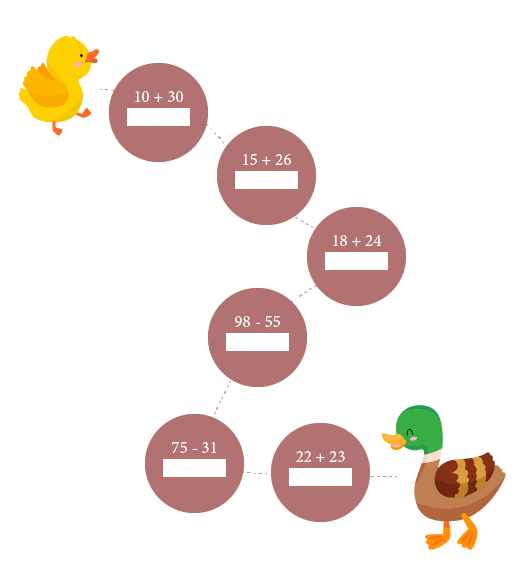
\includegraphics[width=.7\textwidth]{./media/SAEB_1ANO_MAT_FIGURA23.png}
\end{figure}

\rosa{Os resultados são os números de 40 a 45, de cima para baixo.}

\num{6} JOANA TEM MUITA VONTADE DE COMPRAR UMA BOLA NOVA, DEPOIS QUE PERDEU A 
QUE TINHA, E DESCOBRIU QUE, NA LOJA PERTO DE SUA CASA, UMA BEM LEGAL CUSTA 56 
REAIS. A MENINA ABRIU SEU COFRINHO E CONTOU 25 REAIS, MAS JÁ CONTAVA COM A 
MESADA DE 15 REAIS QUE RECEBERIA NO FINAL DA SEMANA. QUANTO AINDA VAI FALTAR 
PARA JOANA COMPRAR A BOLA?

\coment{A menina já tem 25 reais e vai ganhar mais 15.

Ela vai ficar com 25 + 15 = 40 reais.

Para ela comprar a bola de 56 reais,

ainda faltam 56 -- 40 = 16 reais.
}

\vspace{3cm}

\num{7} DEMONSTRE DIFERENTES MODOS DE FORMARMOS O NÚMERO 100 POR MEIO DA ADIÇÃO DE
DUAS PARCELAS.

\vspace{2cm}

\begin{center}
\begin{tabular}{llllllllllllll}
50 &  &  & \mbox{} &  &  & \mbox{} &  &  & \mbox{} &  &  & \mbox{} &  \\
50 & $+$ &  & \mbox{} & $+$ &  & \mbox{} & $+$ &  & \mbox{} & $+$ &  & \mbox{} & $+$ \\ \cline{1-1} \cline{4-4} \cline{7-7} \cline{10-10} \cline{13-13}
100 &  &  & 100 &  &  & 100 &  &  & 100 &  &  & 100 & 
\end{tabular}
\end{center}

\vspace{2cm}

\begin{center}
\begin{tabular}{llllllllllllll}
\mbox{} &  &  & \mbox{} &  &  & \mbox{} &  &  & \mbox{} &  &  & \mbox{} &  \\
\mbox{} & $+$ &  & \mbox{} & $+$ &  & \mbox{} & $+$ &  & \mbox{} & $+$ &  & \mbox{} & $+$ \\ \cline{1-1} \cline{4-4} \cline{7-7} \cline{10-10} \cline{13-13}
100 &  &  & 100 &  &  & 100 &  &  & 100 &  &  & 100 & 
\end{tabular}
\end{center}

\vspace{2cm}

%\coment{Crie alguns exemplos com os alunos e oriente-os a utilizarem números mais simples, como 10, 20 etc. Aproveite para lembrar-lhes o conceito de parcelas, pois, talvez, alguns não saibam ainda o que significa essa palavra. A atividade pode ser aproveitada para ampliar o vocabulário dos alunos.}

\num{8} DEMONSTRE DIFERENTES MODOS DE FORMARMOS O NÚMERO 10 POR MEIO DA SUBTRAÇÃO DE
DUAS PARCELAS.

\vspace{2cm}

\begin{center}
\begin{tabular}{llllllllllllll}
100 &  &  & \mbox{} &  &  & \mbox{} &  &  & \mbox{} &  &  & \mbox{} &  \\
90 & $-$ &  & \mbox{} & $-$ &  & \mbox{} & $-$ &  & \mbox{} & $-$ &  & \mbox{} & $-$ \\ \cline{1-1} \cline{4-4} \cline{7-7} \cline{10-10} \cline{13-13}
10 &  &  & 10 &  &  & 10 &  &  & 10 &  &  & 10 & 
\end{tabular}
\end{center}

\vspace{2cm}

\begin{center}
\begin{tabular}{llllllllllllll}
\mbox{} &  &  & \mbox{} &  &  & \mbox{} &  &  & \mbox{} &  &  & \mbox{} &  \\
\mbox{} & $-$ &  & \mbox{} & $-$ &  & \mbox{} & $-$ &  & \mbox{} & $-$ &  & \mbox{} & $-$ \\ \cline{1-1} \cline{4-4} \cline{7-7} \cline{10-10} \cline{13-13}
10 &  &  & 10 &  &  & 10 &  &  & 10 &  &  & 10 & 
\end{tabular}
\end{center}

\vspace{2cm}

\num{9} RESOLVA O ENIGMA E DESCUBRA QUAL É O NÚMERO.

\begin{itemize}
\item SOU MAIOR QUE 5.

\item SOU MENOR QUE 50.

\item UMA DAS MINHAS PARCELAS PODE SER 12.

\item UMA DAS MINHAS PARCELAS TAMBÉM PODE SER 10.

\item SE UMA DAS MINHAS PARCELAS FOR 20, A OUTRA NÃO PODE SER MAIOR DO QUE 2.
\end{itemize}

% \begin{figure}[htpb!]
% \centering
% 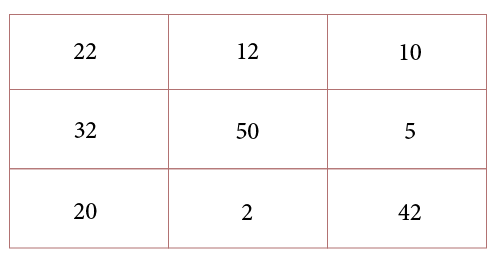
\includegraphics[width=.5\textwidth]{./media/SAEB_1ANO_MAT_FIGURA25.png}
% \end{figure}

\reduline{O número em questão é o 22.\hfill}
\linhas{2}

% \num{10} PINTE DA MESMA COR OS NÚMEROS QUE, ADICIONADOS, EM TRÊS PARCELAS, PODEM
% FORMAR OS NÚMEROS QUE SE PEDEM.

% \begin{figure}[htpb!]
% 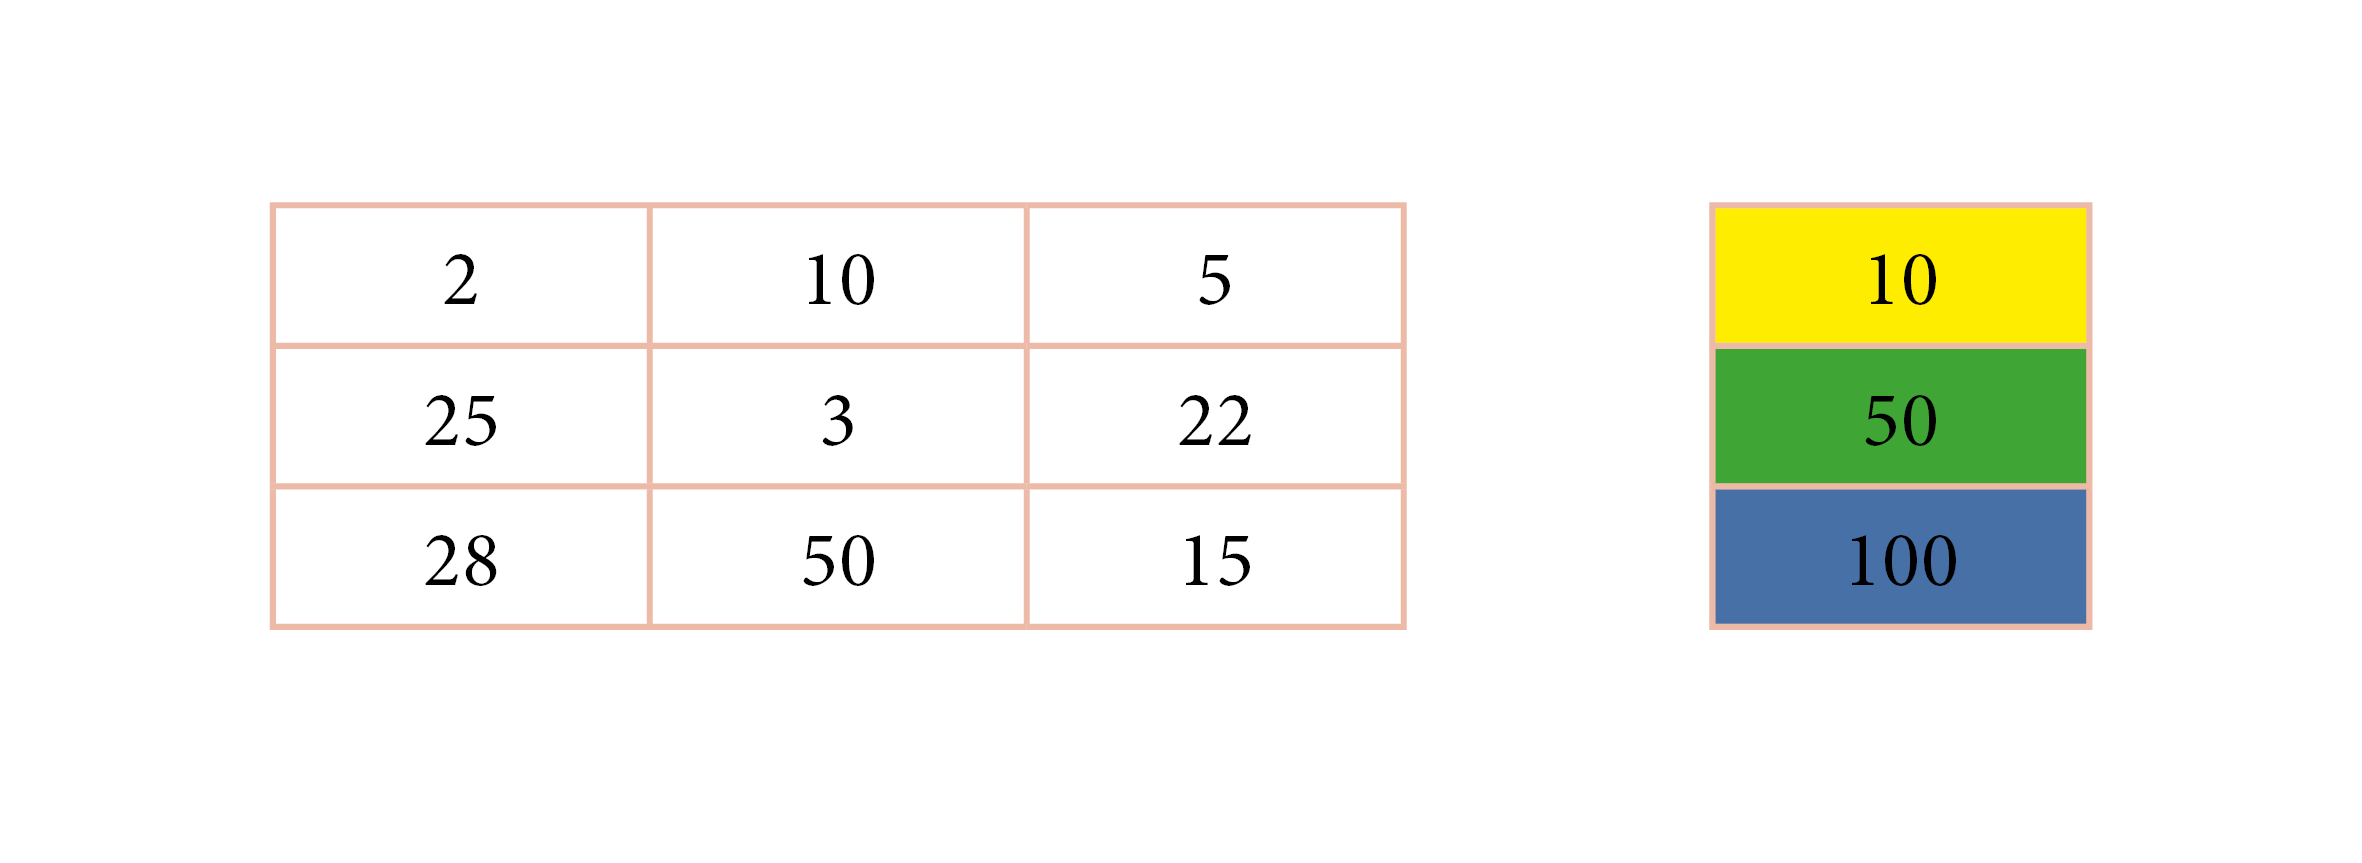
\includegraphics[width=\textwidth]{./media/SAEB_1ANO_MAT_FIGURA26.png}
% \end{figure}

% \rosa{Amarelo: 2, 3, 5. Verde: 10, 15, 25. Azul: 22, 28, 50.}

%Explique aos alunos que só existe uma combinação possível para cada número. Oriente também a pintarem as parcelas na cor equivalente aos resultados esperados na coluna do lado direito. Peça a eles que confiram antes de pintar.

%\coment{As combinações são:
%\begin{longtable}[]{@{}lllll@{}}
%\toprule
%amarelo & verde & amarelo & & \(2 + 3 + 5 = 10\)\tabularnewline
%verde & amarelo & azul & & \(25 + 10 + 15 = 50\)\tabularnewline
%azul & azul & verde & & \(28 + 50 + 22 = 100\)\tabularnewline
%\bottomrule
%\end{longtable}
%}

% \num{11} PATRICK QUER VENDER SEU ÁLBUM DE FIGURINHAS POR 56 REAIS. UM AMIGUINHO
% QUER COMPRÁ-LO, MAS SÓ TEM 13 REAIS. ALÉM DISSO, SÓ PODERA PAGAR O RESTO
% EM DUAS VEZES, E A PRIMEIRA PARCELA DEVERIA SER MENOR QUE A PRIMEIRA.
% ELABORE TRÊS FORMAS DE PAGAMENTO PARA O AMIGO DE PATRICK.

% \begin{figure}[htpb!]
% \centering
% 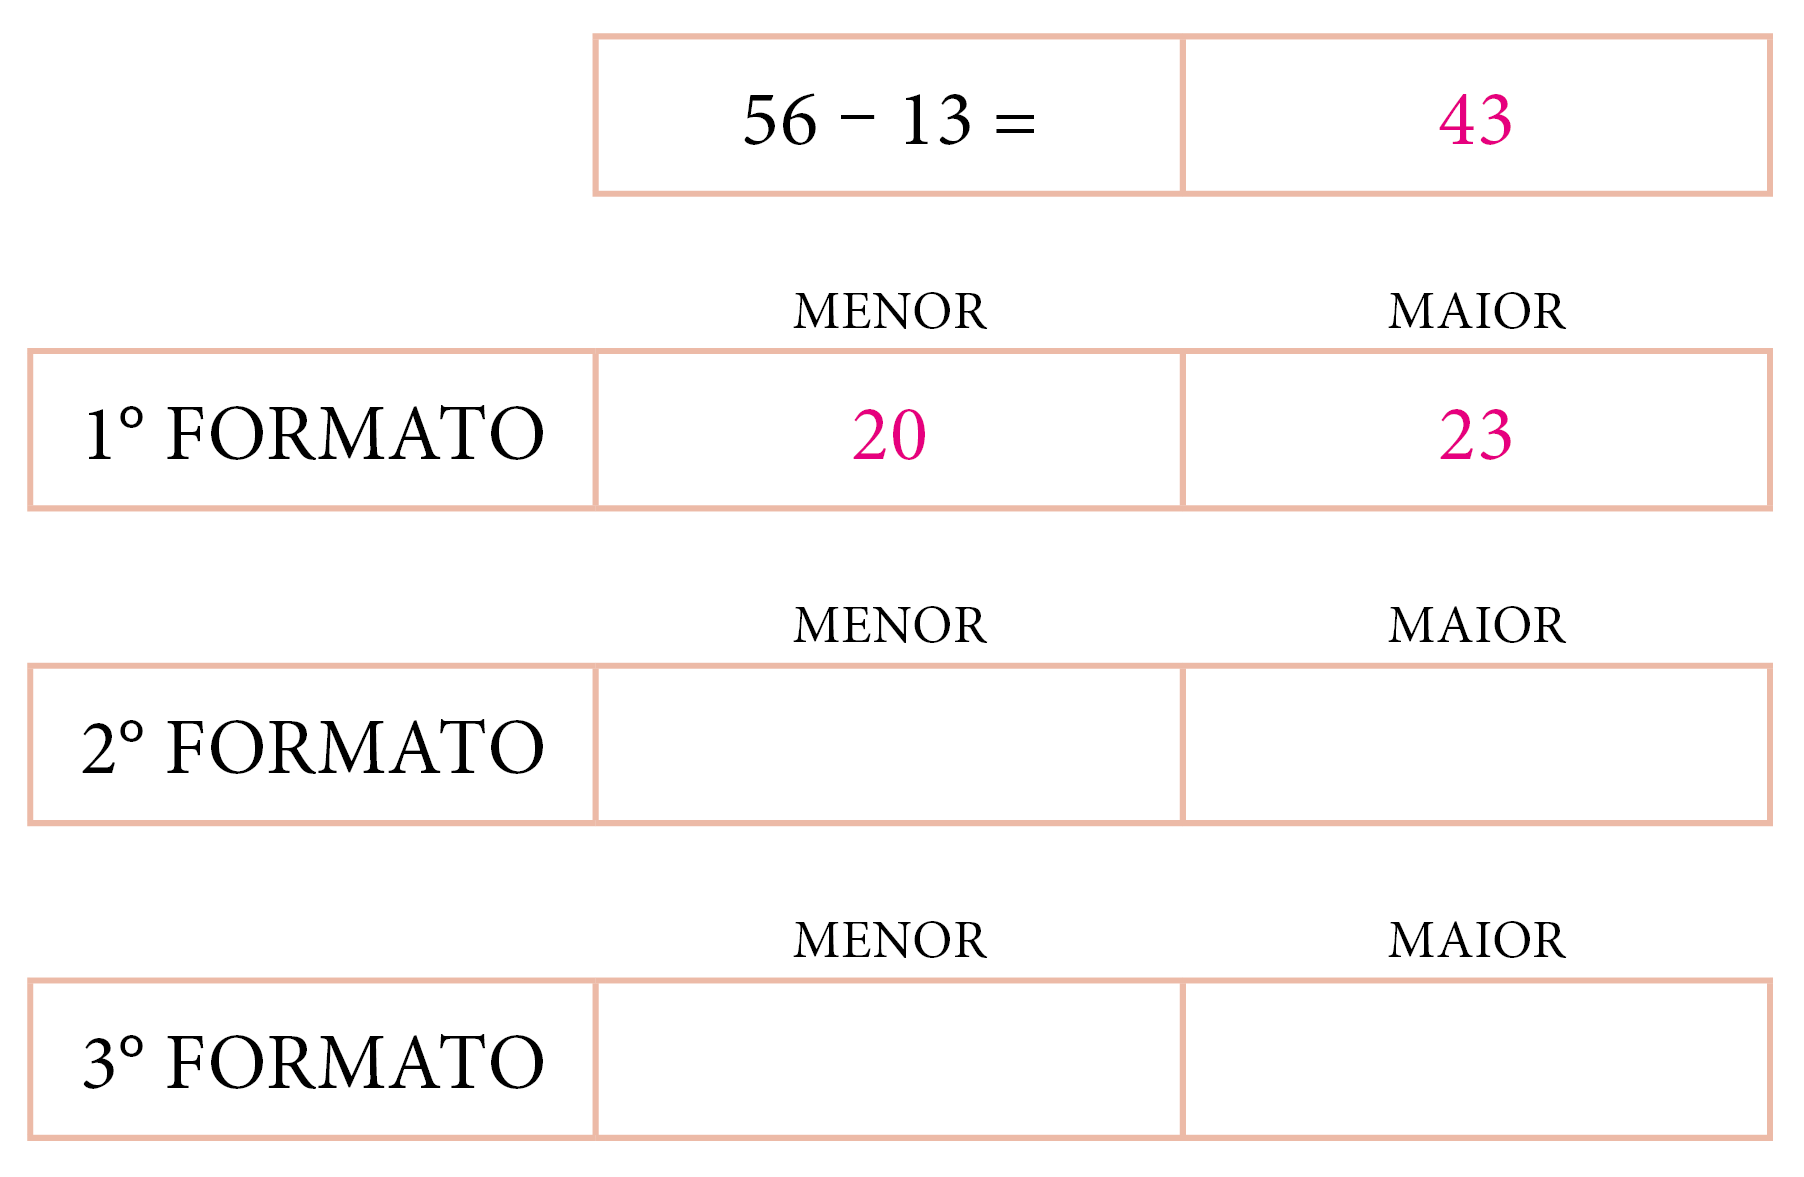
\includegraphics[width=.8\textwidth]{./media/SAEB_1ANO_MAT_FIGURA28.png}
% \end{figure}

% %\coment{Oriente os alunos a primeiro descobrirem quanto falta para o amigo de Patrick pagar pelo álbum de figurinhas.}

% \num{12} ASSINALE UMA FORMA DE AGRUPARMOS 45 REAIS UTILIZANDO AS SEGUINTES
% CÉDULAS.

% %\textless{}Criar uma figura conforme o modelo a seguir. Se necessário desconfigure as notas de reais, contanto que as cédulas fictícias tenham o mesmo valor. Coloque uma bola para que o aluno assinale. 

% \begin{minipage}{.8\textwidth}
% 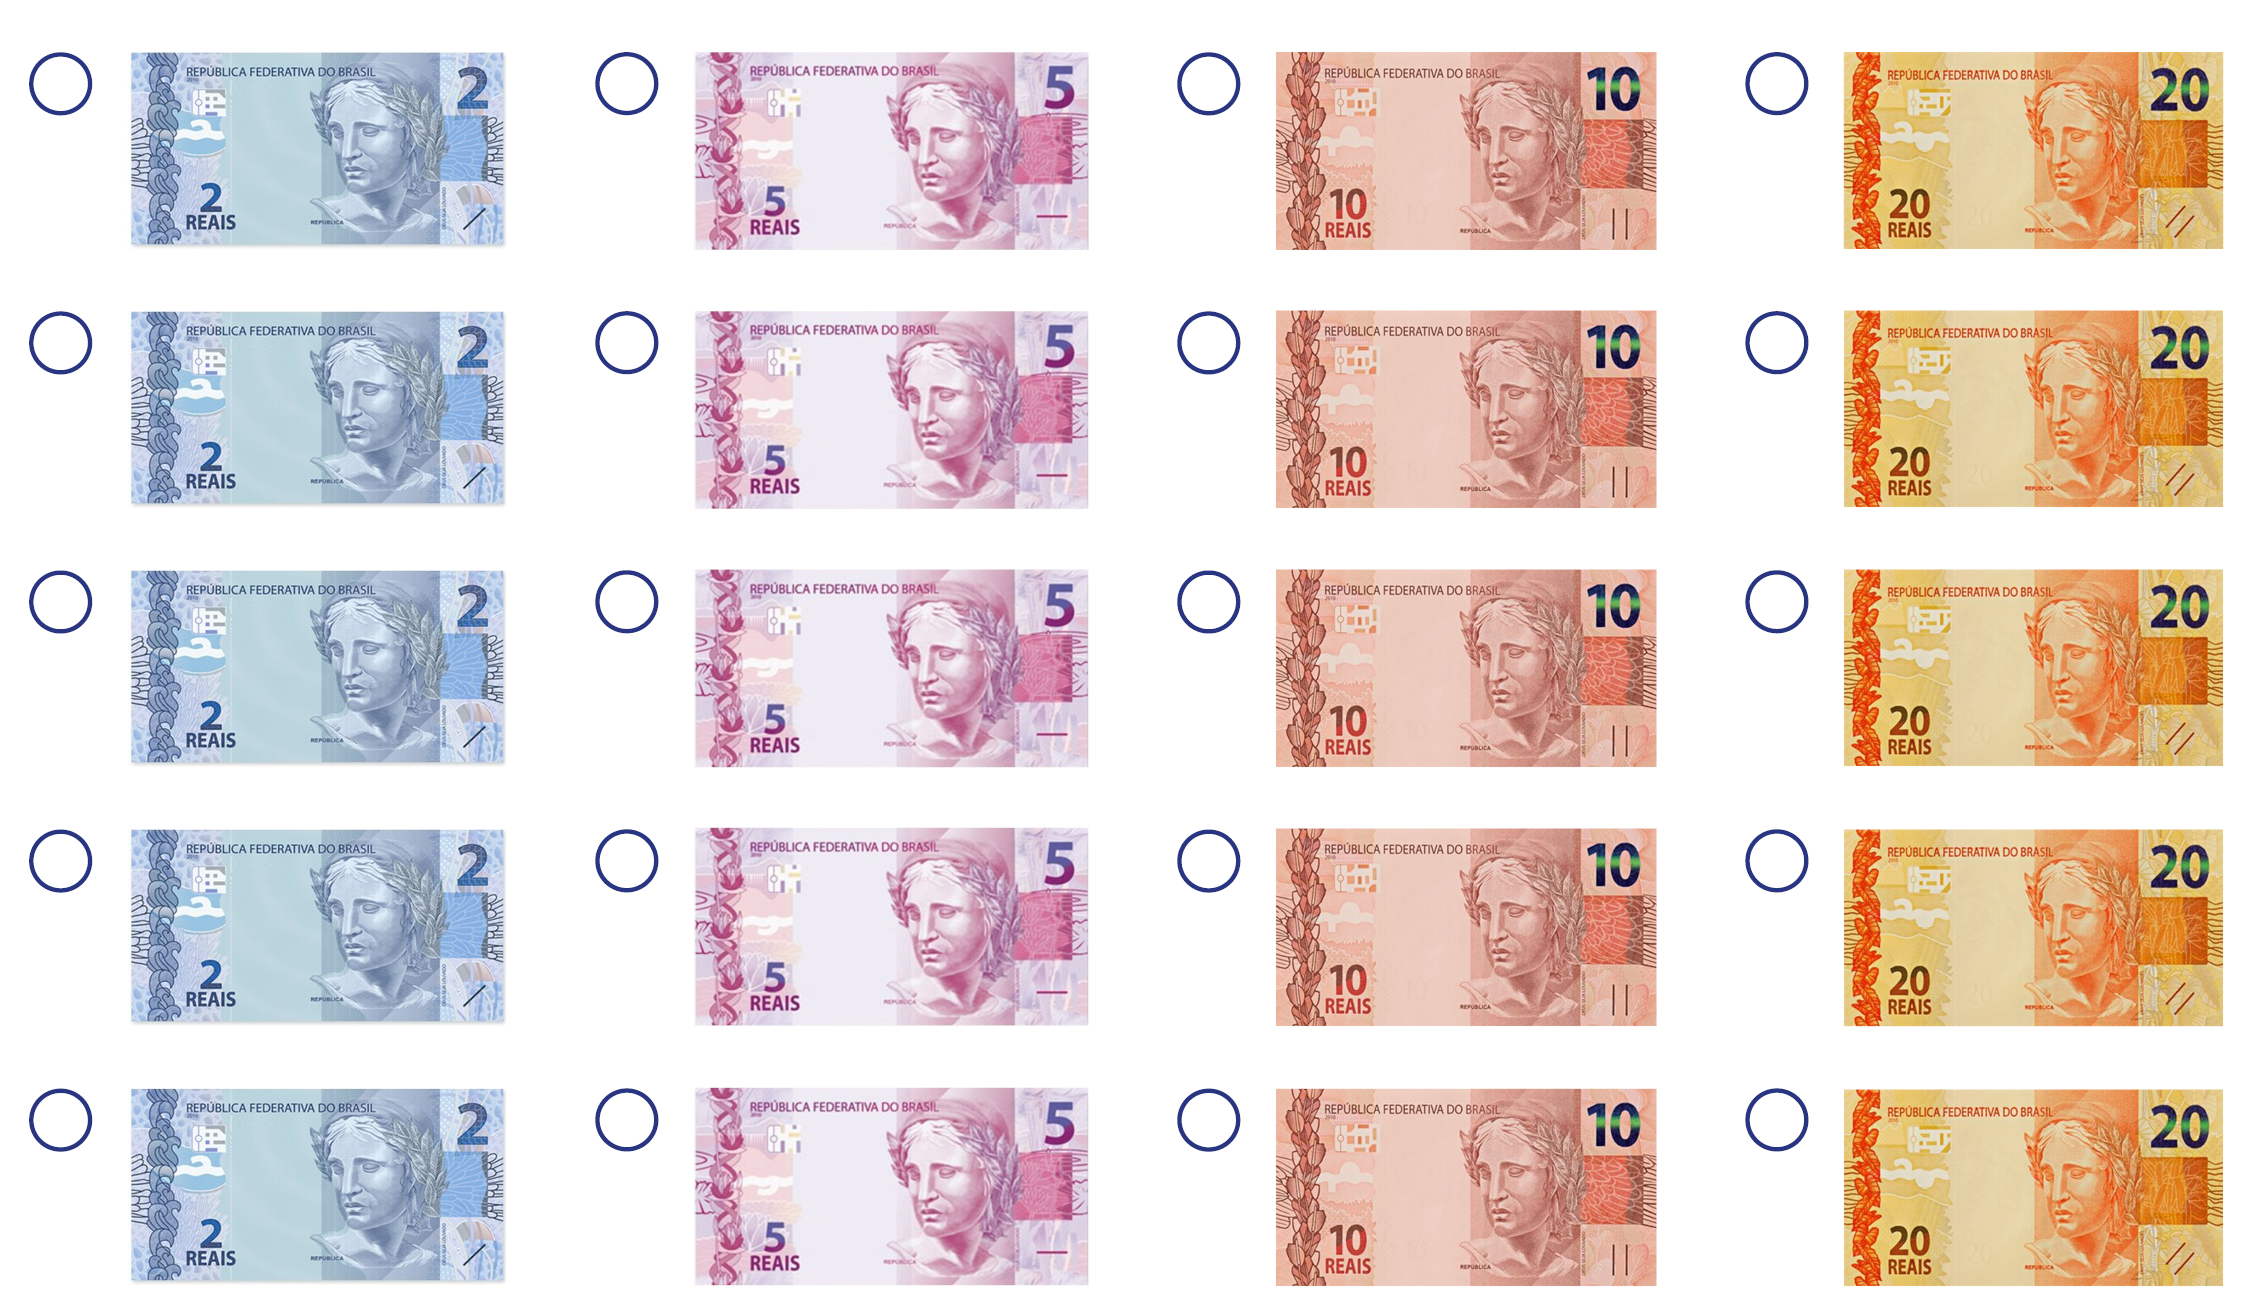
\includegraphics[width=\textwidth]{./media/SAEB_1ANO_MAT_FIGURA29.png}
% \end{minipage}
% \begin{minipage}{.3\textwidth}
% \coment{Há várias respostas possíveis. É
% importante que o aluno consiga compreender a ideia de composição por
% diferentes adições. Peça às crianças que criem outra forma além da
% encontrada na atividade e registrem na lousa. Esta atividade é
% importante para trabalhar educação financeira. Algumas das combinações
% podem ser: (20 + 20 + 5,\ \ \ \ 10 + 10 + 10 + 10 + 5), 2 + 2 + 2 + 2 + 2 + 10 + 20 + 5 etc.}
% \end{minipage}

% \pagebreak
% \num{13} NUMA PARTIDA DE FUTEBOL, ESTAVAM JOGANDO DOIS TIMES: O TIME A E O TIME B. FORAM MARCADOS 10 GOLS, E O TIME A VENCEU A PARTIDA. IDENTIDIQUE OS POSSÍVEIS PLACARES.

% %\textless{}Inserir uma figura conforme o modelo a seguir. https://br.freepik.com/vetores-gratis/conjunto-de-simbolos-ou-emblemas-de-escudo-de-nove\_8998384.htm\#query=escudo\%20de\%20time\&position=5\&from\_view=search\&track=ais.\textgreater{}

% \begin{figure}[htpb!]
% \centering
% 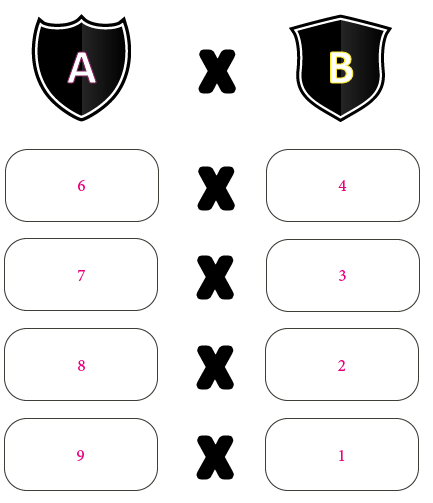
\includegraphics[width=.6\textwidth]{./media/SAEB_1ANO_MAT_FIGURA30.png}
% \end{figure}

% %\coment{Oriente os alunos sobre o fato de haver exatamente quatro resultados possíveis.}

% \num{14} A MÃE DE REINALDO VAI CHAMAR 50 PESSOAS PARA A FESTA DE ANIVERSÁRIO DELE,
% MAS REINALDO TEM 10 TIOS, 8 TIAS, 15 PRIMOS, 9 AMIGOS E 4 VIZINHOS. SOBRE ESSA SITUAÇÃO, RESPONDA AO QUE SE PERGUNTA A SEGUIR.

% \begin{escolha}
% \item CONVIDANDO-SE TODAS ESSAS PESSOAS MENCIONADAS, PODEM-SE ACRESCENTAR CONVIDADOS OU SERÁ NECESSÁRIO RETIRAR PESSOAS DA LISTA?

% \reduline{O aluno precisa somar o número de pessoas: (10 + 8 + 15 + 9 + 4 = 46). Com isso, ele descobre que se podem acrescentar quatro pessoas ainda.\hfill}

% \item QUANTOS CONVIDADOS PODEM SER ACRESCENTADOS OU QUANTAS PESSOAS PRECISAM SER
%   RETIRADAS?

% \reduline{Subtraindo-se o número de pessoas da lista do número de convites para a festa, tem-se: (50 - 46 = 4). Podem ser convidadas ainda outras quatro pessoas.\hfill}
% \end{escolha}

% \num{15} ANALISE AS CAIXAS COM AS FIGURAS GEOMÉTRICAS. PRECISAMOS ORGANIZÁ-LAS PARA QUE CADA CAIXA TENHA A MESMA QUANTIDADE DE FIGURAS. SÃO 16 CÍRCULOS, 16 QUADRADOS E 16 TRIÂNGULOS; ENTÃO CADA CAIXA DEVE CONTER 4 QUADRADOS, 4 TRIÂNGULOS E 4 CÍRCULOS.

% %\textless{}Inserir uma figura com quatro caixas, identificadas por letras, contendo círculos, quadrados e triângulos, espalhados de forma aleatória, conforme o modelo a seguir.

% \begin{figure}[htpb!]
% \centering
% 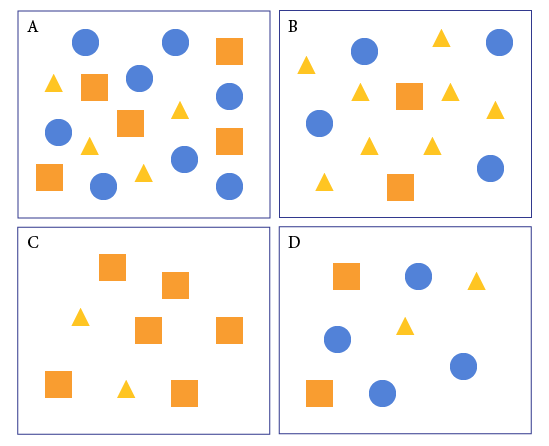
\includegraphics[width=.5\textwidth]{./media/SAEB_1ANO_MAT_FIGURA31.png}
% \end{figure}

% \begin{escolha}
% \item QUANTOS CÍRCULOS DEVEM SER RETIRADOS DA CAIXA \textbf{A}?

% \reduline{2  círculos.\hfill}

% \item QUANTOS TRIÂNGULOS DEVEM SER RETIRADOS DA CAIXA \textbf{B}?

% \reduline{4 triângulos.\hfill}

% \item QUANTOS TRIÂNGULOS DEVEM SER ADICIONADOS ÀS CAIXAS \textbf{C} E \textbf{D}?

% \reduline{2 triângulos a cada uma.\hfill}

% \item QUANTOS QUADRADOS DEVEM SER RETIRADOS DA CAIXA \textbf{A}?

% \reduline{1 quadrado.\hfill}

% \item QUANTOS QUADRADOS DEVEM SER RETIRADOS DA CAIXA \textbf{C}?

% \reduline{2 quadrados.\hfill}

% \item QUANTOS QUADRADOS DEVEM SER ADICIONADOS ÀS CAIXAS \textbf{B} E \textbf{D}?

% \reduline{2 quadrados a cada uma.\hfill}

% \item CRIANDO-SE UMA QUINTA CAIXA (\textbf{E}), COM TODAS AS FIGURAS JUNTAS, ESSA CAIXA \textbf{E} FICARIA COM QUANTAS FIGURAS?

% \reduline{(16 + 16 + 16 + 16 = 64) figuras.\hfill}
% \end{escolha}

\section*{TREINO}

\num{1} BENÍCIO E BERNARDO SÃO IRMÃOS E RESOLVERAM JUNTAR TODAS AS
SUAS FIGURINHAS: AS 25 DE BENÍCIO E AS 32 DE BERNARDO. QUANTAS FIGURINHAS OS
IRMÃOS TÊM JUNTOS?

\begin{multicols}{2}
\begin{escolha}
\item
  7.
\item
  25.
\item
  32.
\item
  57.
\end{escolha}
\end{multicols}

\num{2} EM UM COLÉGIO, O PRIMEIRO ANO DIVIDIU-SE EM DOIS TIMES PARA JOGAREM BASQUETE: O TIME \textbf{PEQUENOS CAMPEÕES} E O TIME \textbf{BASQUETEIROS}. AO TODO, NO JOGO, OS DOIS TIMES FIZERAM 30 CESTAS, E OS PEQUENOS CAMPEÕES VENCERAM OS BASQUETEIROS. ENTRE AS OPÇÕES A SEGUIR, QUAL FOI O PLACAR FINAL DA PARTIDA?

\begin{escolha}
\item
  PEQUENOS CAMPEÕES 16 X BASQUETEIROS 15.
\item
  PEQUENOS CAMPEÕES 16 X BASQUETEIROS 14.
\item
  PEQUENOS CAMPEÕES 15 X BASQUETEIROS 14.
\item
  PEQUENOS CAMPEÕES 15 X BASQUETEIROS 13.
\end{escolha}

\num{3} VINÍCIUS QUER COMPRAR UM LANCHE, MAS SÓ TEM 15 REAIS. PEDIU A SUA MÃE, E
ELA LHE DEU MAIS 12 REAIS. DEPOIS, PEDIU DINHEIRO À AVÓ, E ELA
LHE DEU MAIS 10 REAIS. ENTÃO, VINÍCIUS PERCEBEU QUE CONSEGUIRIA COMPRAR O LANCHE E UM 
SORVETE DE 5 REAIS. QUAL É O PREÇO DO LANCHE?

\begin{multicols}{2}
\begin{escolha}
\item
  15.
\item
  32.
\item
  37.
\item
  42.
\end{escolha}
\end{multicols}

\chapter{MAMÃE, ESTOU CRESCENDO!}
\markboth{Módulo 3}{}

%\coment{Neste módulo, vamos desenvolver as habilidades relativas aos conceitos de massa, volume e comprimento. Desenvolver nos alunos a ideia da necessidade de criarmos padrões de comparação para que medidas sejam feitas com cada vez mais precisão.}

\section*{HABILIDADES DO SAEB}

\begin{itemize}
\item
  \uppercase{Comparar comprimentos, capacidades ou massas ou ordenar imagens de
  objetos com base na comparação visual de seus comprimentos,
  capacidades ou massas.}
\item
  \uppercase{Estimar/inferir medida de comprimento, capacidade ou massa de objetos,
  utilizando unidades de medida convencionais ou não ou medir
  comprimento, capacidade ou massa de objetos.}
\item
  \uppercase{Identificar a medida de comprimento, da capacidade ou da massa de
  objetos, dada a imagem de um instrumento de medida.}
\item
  \uppercase{Reconhecer unidades de medida e/ou instrumentos utilizados para medir
  comprimento, tempo, massa ou capacidade.}
\end{itemize}

\subsection{Habilidade da BNCC}

\begin{itemize}
\item EF01MA15.
\end{itemize}



\conteudo{
% \begin{wrapfigure}{l}{.3\textwidth}
% 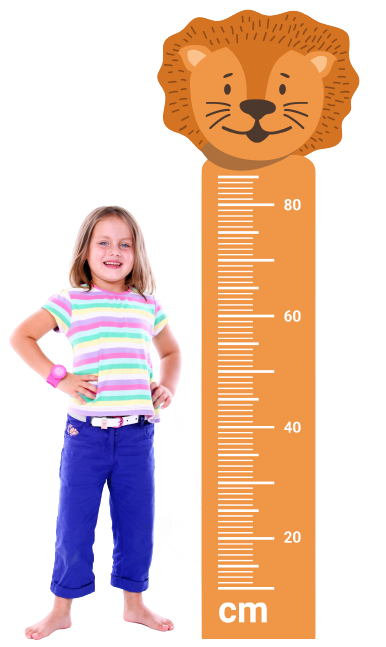
\includegraphics[width=.2\textwidth]{./media/SAEB_1ANO_MAT_FIGURA32.png}
% \end{wrapfigure}

MARIANA ESTÁ AGORA COM CERCA DE 1 METRO DE \textbf{ALTURA}.

% \begin{center}
% 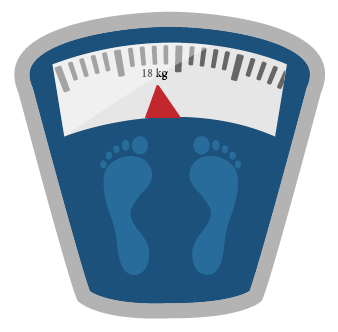
\includegraphics[width=.6\textwidth]{./media/SAEB_1ANO_MAT_FIGURA33.png}
% \end{center}

A MENINA ESTÁ AGORA COM CERCAD DE 14 QUILOGRAMAS DE \textbf{MASSA},
COMO UM EXTINTOR DE INCÊNDIO, MAS COMO DOIS CORPOS TÃO DIFERENTES
PODEM TER A MESMA MASSA?
CADA CORPO TEM UMA CAPACIDADE DIFERENTE DE OCUPAR
ESPAÇO. ESSA CAPACIDADE É O QUE CHAMAMOS DE \textbf{VOLUME}.

PARA MEDIRMOS COMPRIMENTOS, USAMOS A UNIDADE \textbf{METRO}, POR EXEMPLO.
PARA MEDIRMOS MASSAS, USAMOS A MEDIDA \textbf{QUILOGRAMA}, POR EXEMPLO. 
PARA MEDIRMOS O VOLUME, USAMOS A MEDIDA \textbf{LITRO}, POR EXEMPLO.
}

\section*{ATIVIDADES}

\num{1} DIFERENCIE O QUE COMPRAMOS POR QUILOGRAMA, POR LITRO OU POR UNIDADE.

%\textless{} https://br.freepik.com/vetores-premium/compra-de-mantimentos-frescos\_19552867.htm\#query=market\%20products\&position=9\&from\_view=search\&track=ais

\begin{figure}[H]
\centering
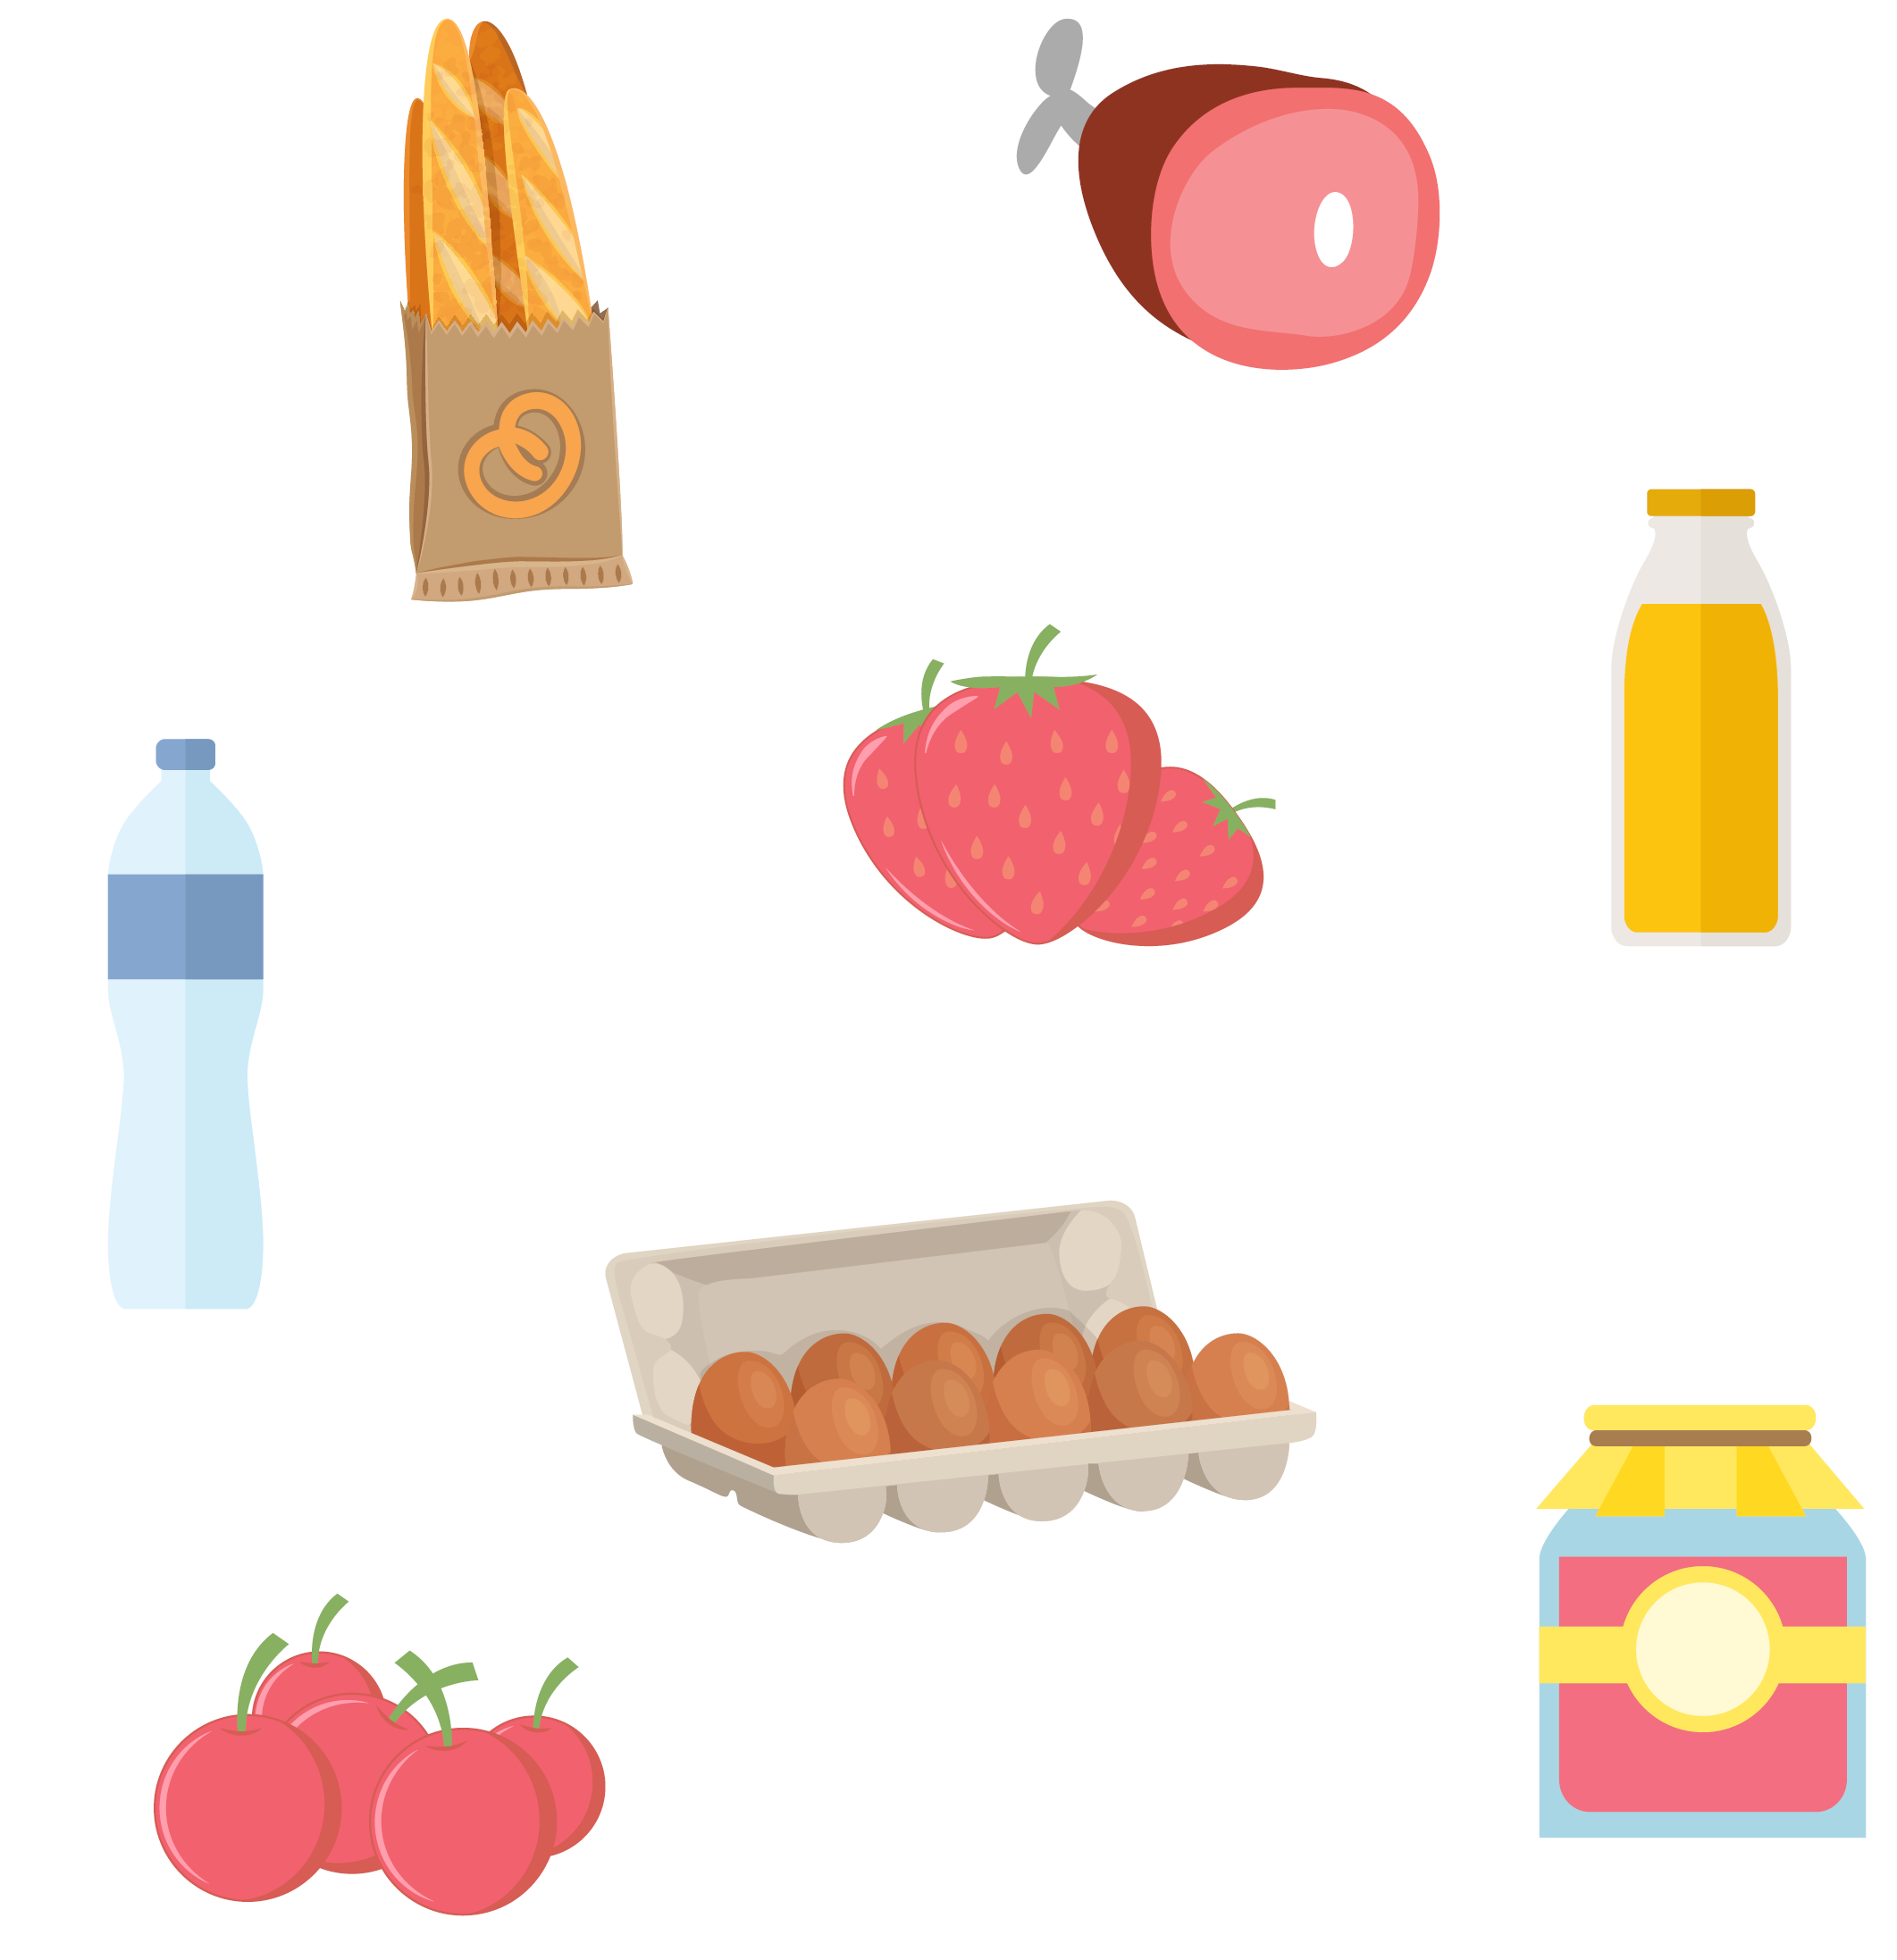
\includegraphics[width=.65\textwidth]{./media/SAEB_1ANO_MAT_FIGURA34.png}
\end{figure}

\rosa{Quilograma: carne, pão, frutas. Litro: água, suco. Unidade: ovo, geleia.}

\bigskip

\num{2} CIRCULE E DESCREVA OS ITENS QUE PODEM SER MEDIDOS EM METROS.\bigskip

%\textless{}Crie a figura conforme o modelo, utilizando as referências: https://br.freepik.com/vetores-premium/mesa-de-madeira\_31804490.htm\#query=mesa\%20desenho\&position=5\&from\_view=search\&track=ais; https://br.freepik.com/vetores-gratis/adesivo-de-pacote-de-saco-de-acucar-em-fundo-branco\_18055550.htm\#query=a\%C3\%A7ucar\%20desenho\&position=2\&from\_view=search\&track=ais (traduzir -- açúcar); https://br.freepik.com/vetores-gratis/fatia-de-queijo-saboroso\_3077481.htm\#query=queijo\%20desenho\&position=7\&from\_view=search\&track=ais; https://br.freepik.com/vetores-gratis/beber\_23715247.htm\#query=refri\%20desenho\&position=9\&from\_view=search\&track=ais; https://br.freepik.com/vetores-gratis/desenho-de-adesivo-com-rolo-de-corda-isolado\_18184169.htm\#query=cordadesenho\&position=0\&from\_view=search\&track=ais; \href{https://br.freepik.com/vetores-premium/oleo-de-motor-de-substituicao-mecanico-de-automoveis-segurando-uma-lata-de-oleo-de-motor-isolado-no-fundo-branco-manutencao-do-servico-da-estacao-motor-e-mecanismos-de-lubrificacao-design-plano-de-ilustracao-vetorial_23005619.htm\#query=gasolina\%20gal\%C3\%A3odesenho\&position=6\&from_view=search\&track=ais}{\emph{https://br.freepik.com/vetores-premium/oleo-de-motor-de-substituicao-mecanico-de-automoveis-segurando-uma-lata-de-oleo-de-motor-isolado-no-fundo-branco-manutencao-do-servico-da-estacao-motor-e-mecanismos-de-lubrificacao-design-plano-de-ilustracao-vetorial\_23005619.htm\#query=gasolina\%20gal\%C3\%A3odesenho\&position=6\&from\_view=search\&track=ais}}.\textgreater{} 

\begin{figure}[H]
\centering
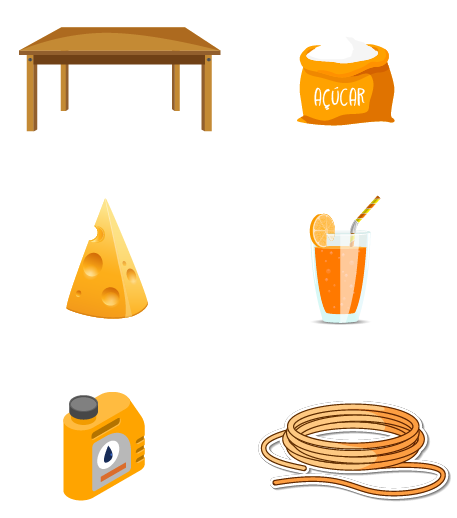
\includegraphics[width=\textwidth]{./media/SAEB_1ANO_MAT_FIGURA35.png}
\end{figure}

\reduline{Somente a mesa e a corda podem ser medidas em metro.\hfill}
\linhas{2}

\num{3} LIGUE CADA PRODUTO À UNIDADE MAIS ADEQUADA PARA MEDI-LO.
DEPOIS, ESCOLHA UM PRODUTO E REGISTRE UMA MEDIÇÃO QUE VOCÊ ENCONTRAR
EM SEU DIA A DIA.

%\textless{}Inserir quadro conforme o modelo a seguir.\textgreater{}

\begin{figure}[H]
\centering
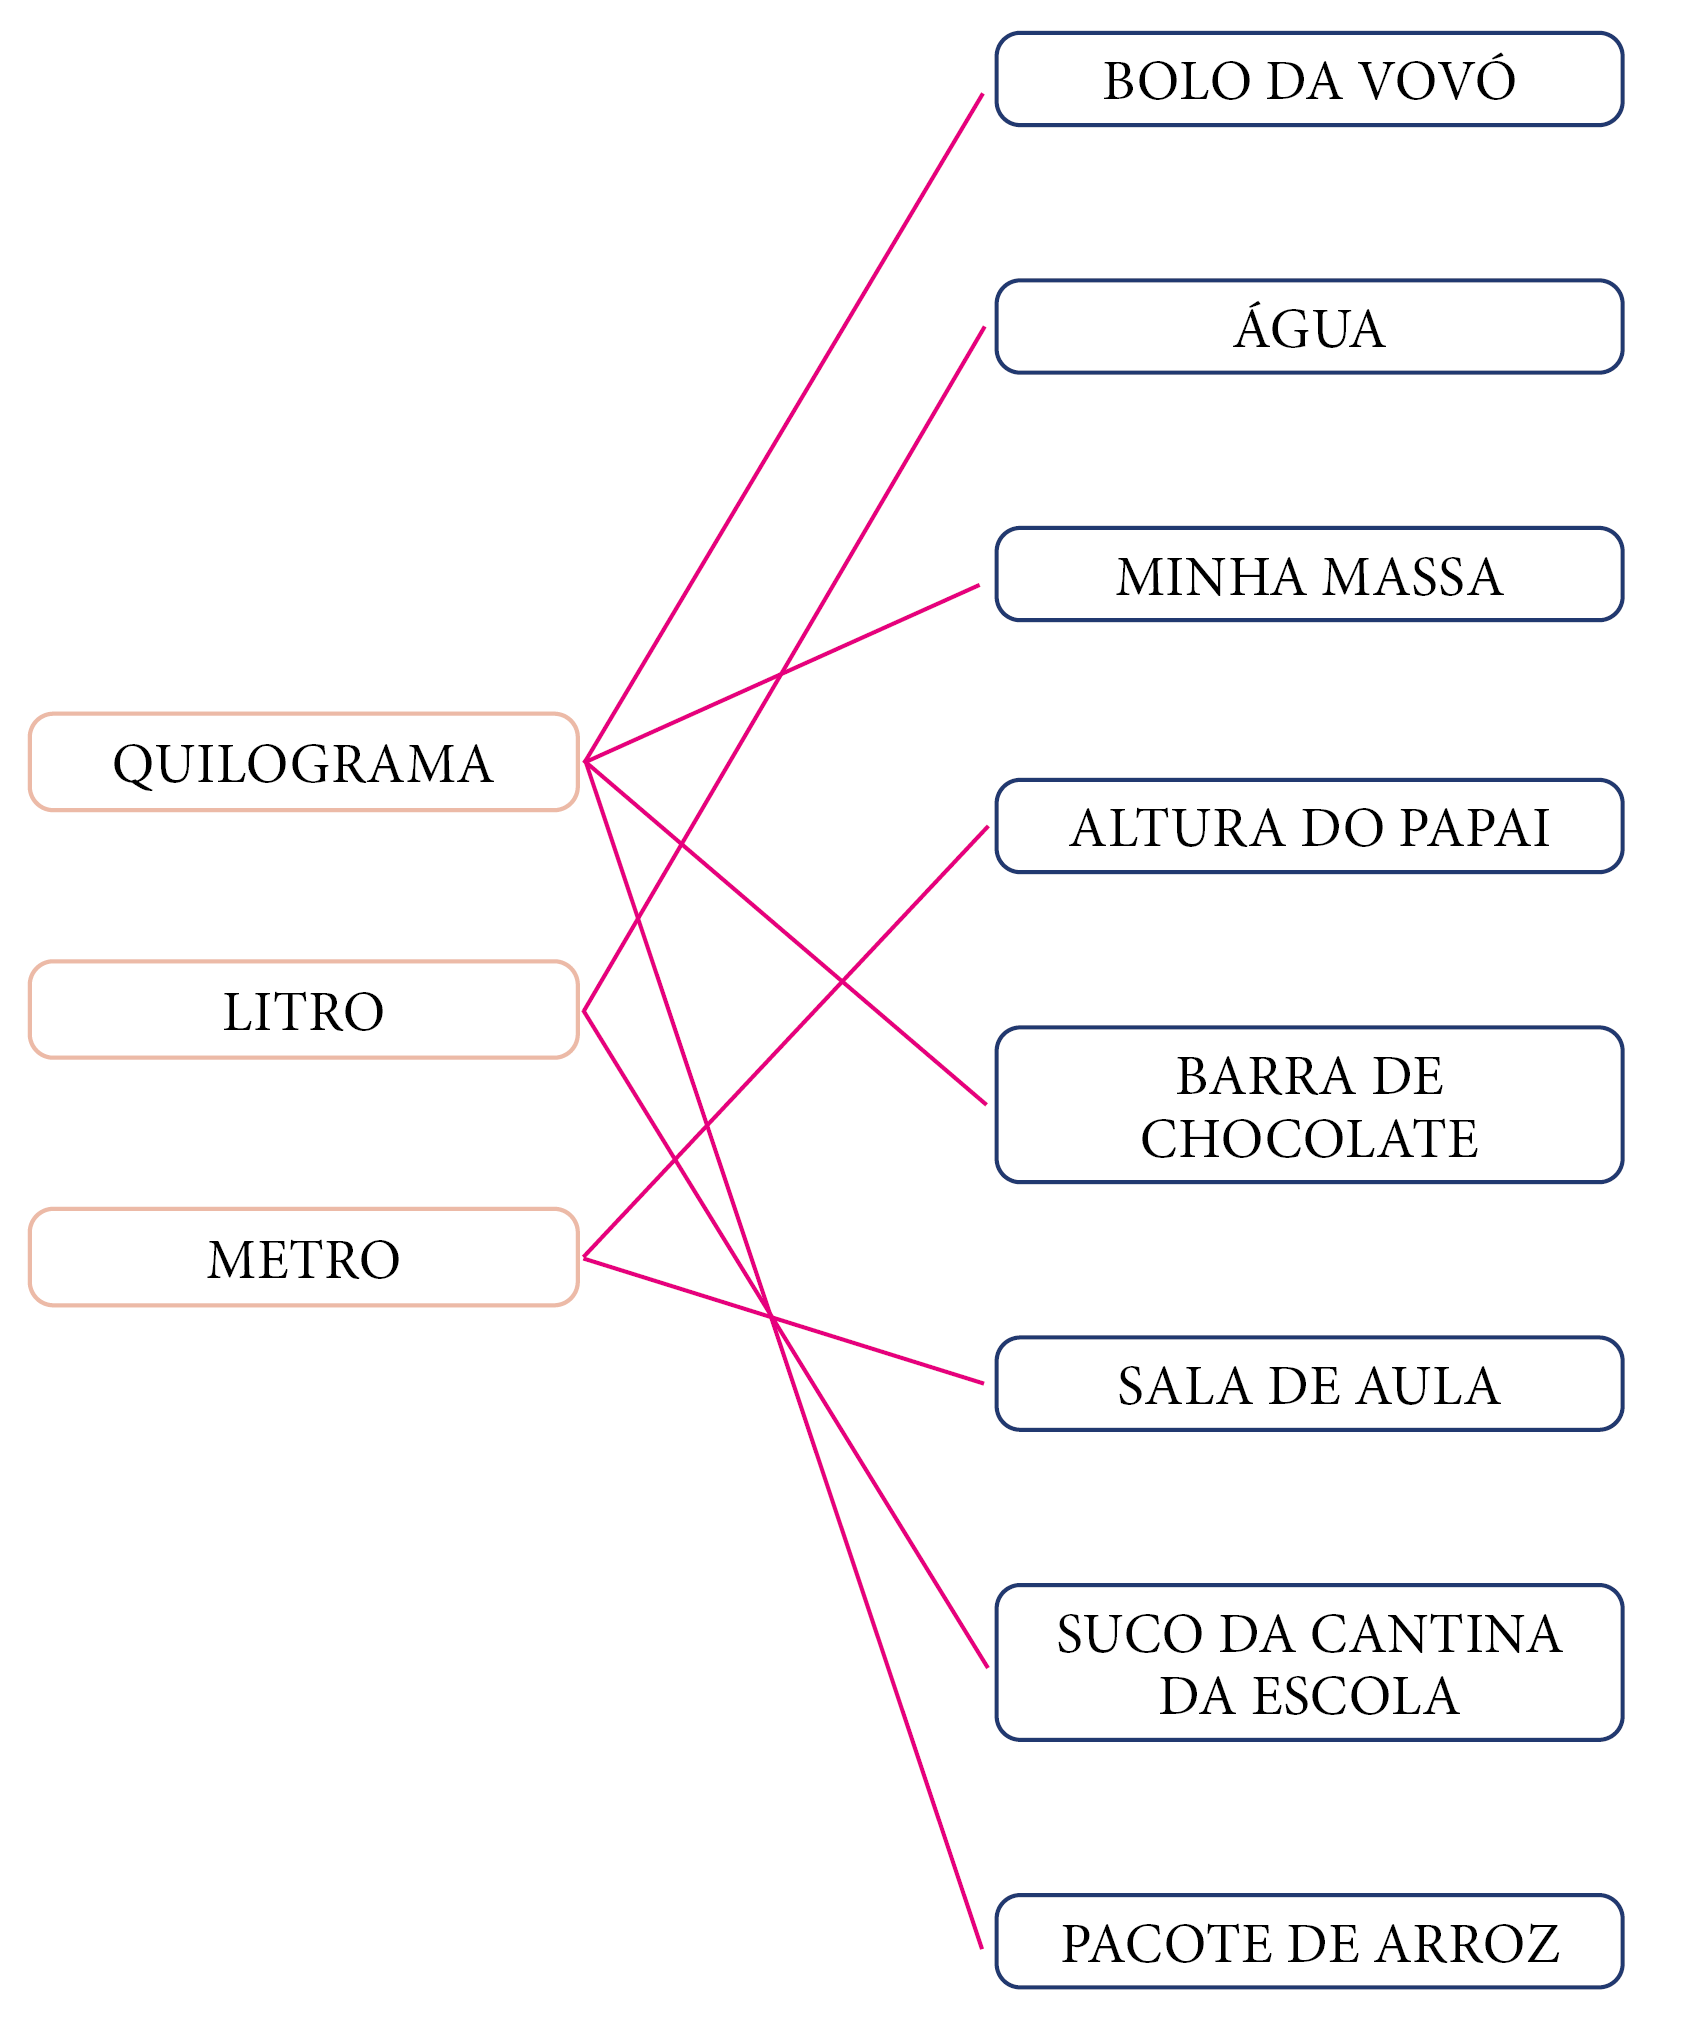
\includegraphics[width=\textwidth]{./media/SAEB_1ANO_MAT_FIGURA36.png}
\end{figure}

\reduline{Resposta circunstancial.\hfill}

\num{4} EM CADA QUADRO A SEGUIR, DESENHE ALGO QUE POSSA SER MEDIDO COM O INSTRUMENTO REPRESENTADO.

%\textless{} insira os quadros e as figuras, conforme o modelo a seguir, utilizando as referências: https://br.freepik.com/vetores-premium/bonito-governante-engracado-acenando-o-personagem-de-mao\_23415941.htm\#page=3\&query=UMA\%20R\%C3\%89GUA\%20DESENHO\&position=39\&from\_view=search\&track=ais; https://br.freepik.com/vetores-gratis/balanca-digital-em-fundo-branco\_16262850.htm\#query=BALAN\%C3\%87A\%20DESENHO\&position=3\&from\_view=search\&track=ais; https://br.freepik.com/vetores-gratis/adesivo-de-copo-de-medicao-em-fundo-branco\_18180135.htm\#query=COPO\%20MEDIDORDESENHO\&position=2\&from\_view=search\&track=ais; https://br.freepik.com/vetores-premium/fita-metrica-para-medir-a-distancia-em-centimetros-e-milimetros-rabiscar-a-coloracao-linear-dos-desenhos-animados\_30247681.htm\#query=TRENA\%20DESENHO\&position=45\&from\_view=search\&track=ais.\textgreater{}

\begin{figure}[H]
\centering
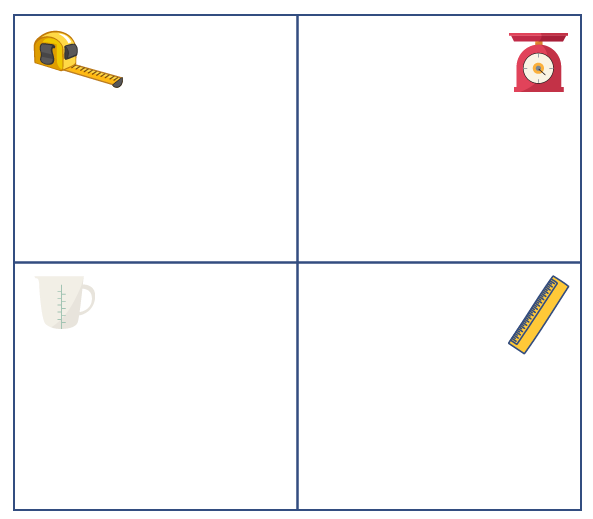
\includegraphics[width=.63\textwidth]{./media/SAEB_1ANO_MAT_FIGURA37.png}
\end{figure}

\num{5} LIGUE CADA PESSOA À SUA CAMA.

%\textless{}Crie um quadro conforme o modelo a seguir, utilizando as referências: https://br.freepik.com/vetores-premium/homem-segurando-binoculos-pessoa-olhando-para-o-horizonte-futuro\_30928646.htm\#query=adulto\%20alto\%20DESENHO\&position=6\&from\_view=search\&track=ais; https://br.freepik.com/vetores-premium/rapaz-dos-desenhos-animados-com-guitarra-criancas-tocando-instrumento-musical-em-casa-aula-ou-performance-artista-de-educacao-musical-ou-ferramentas-de-som-publicidade-vector-hobby-carreira-e-ilustracao-de-atividade-de-lazer\_26152103.htm\#query=adulto\%20baixo\%20DESENHO\&position=8\&from\_view=search\&track=ais; https://br.freepik.com/vetores-gratis/personagem-de-desenho-animado-de-menino-bonito-em-fundo-branco\_28457881.htm\#query=menino\%20DESENHO\&position=5\&from\_view=search\&track=ais; https://br.freepik.com/vetores-gratis/cama-com-travesseiro-e-lencol-azul\_2204447.htm\#query=cama\%20DESENHO\&position=1\&from\_view=search\&track=ais.\textgreater{}

\begin{figure}[H]
\centering
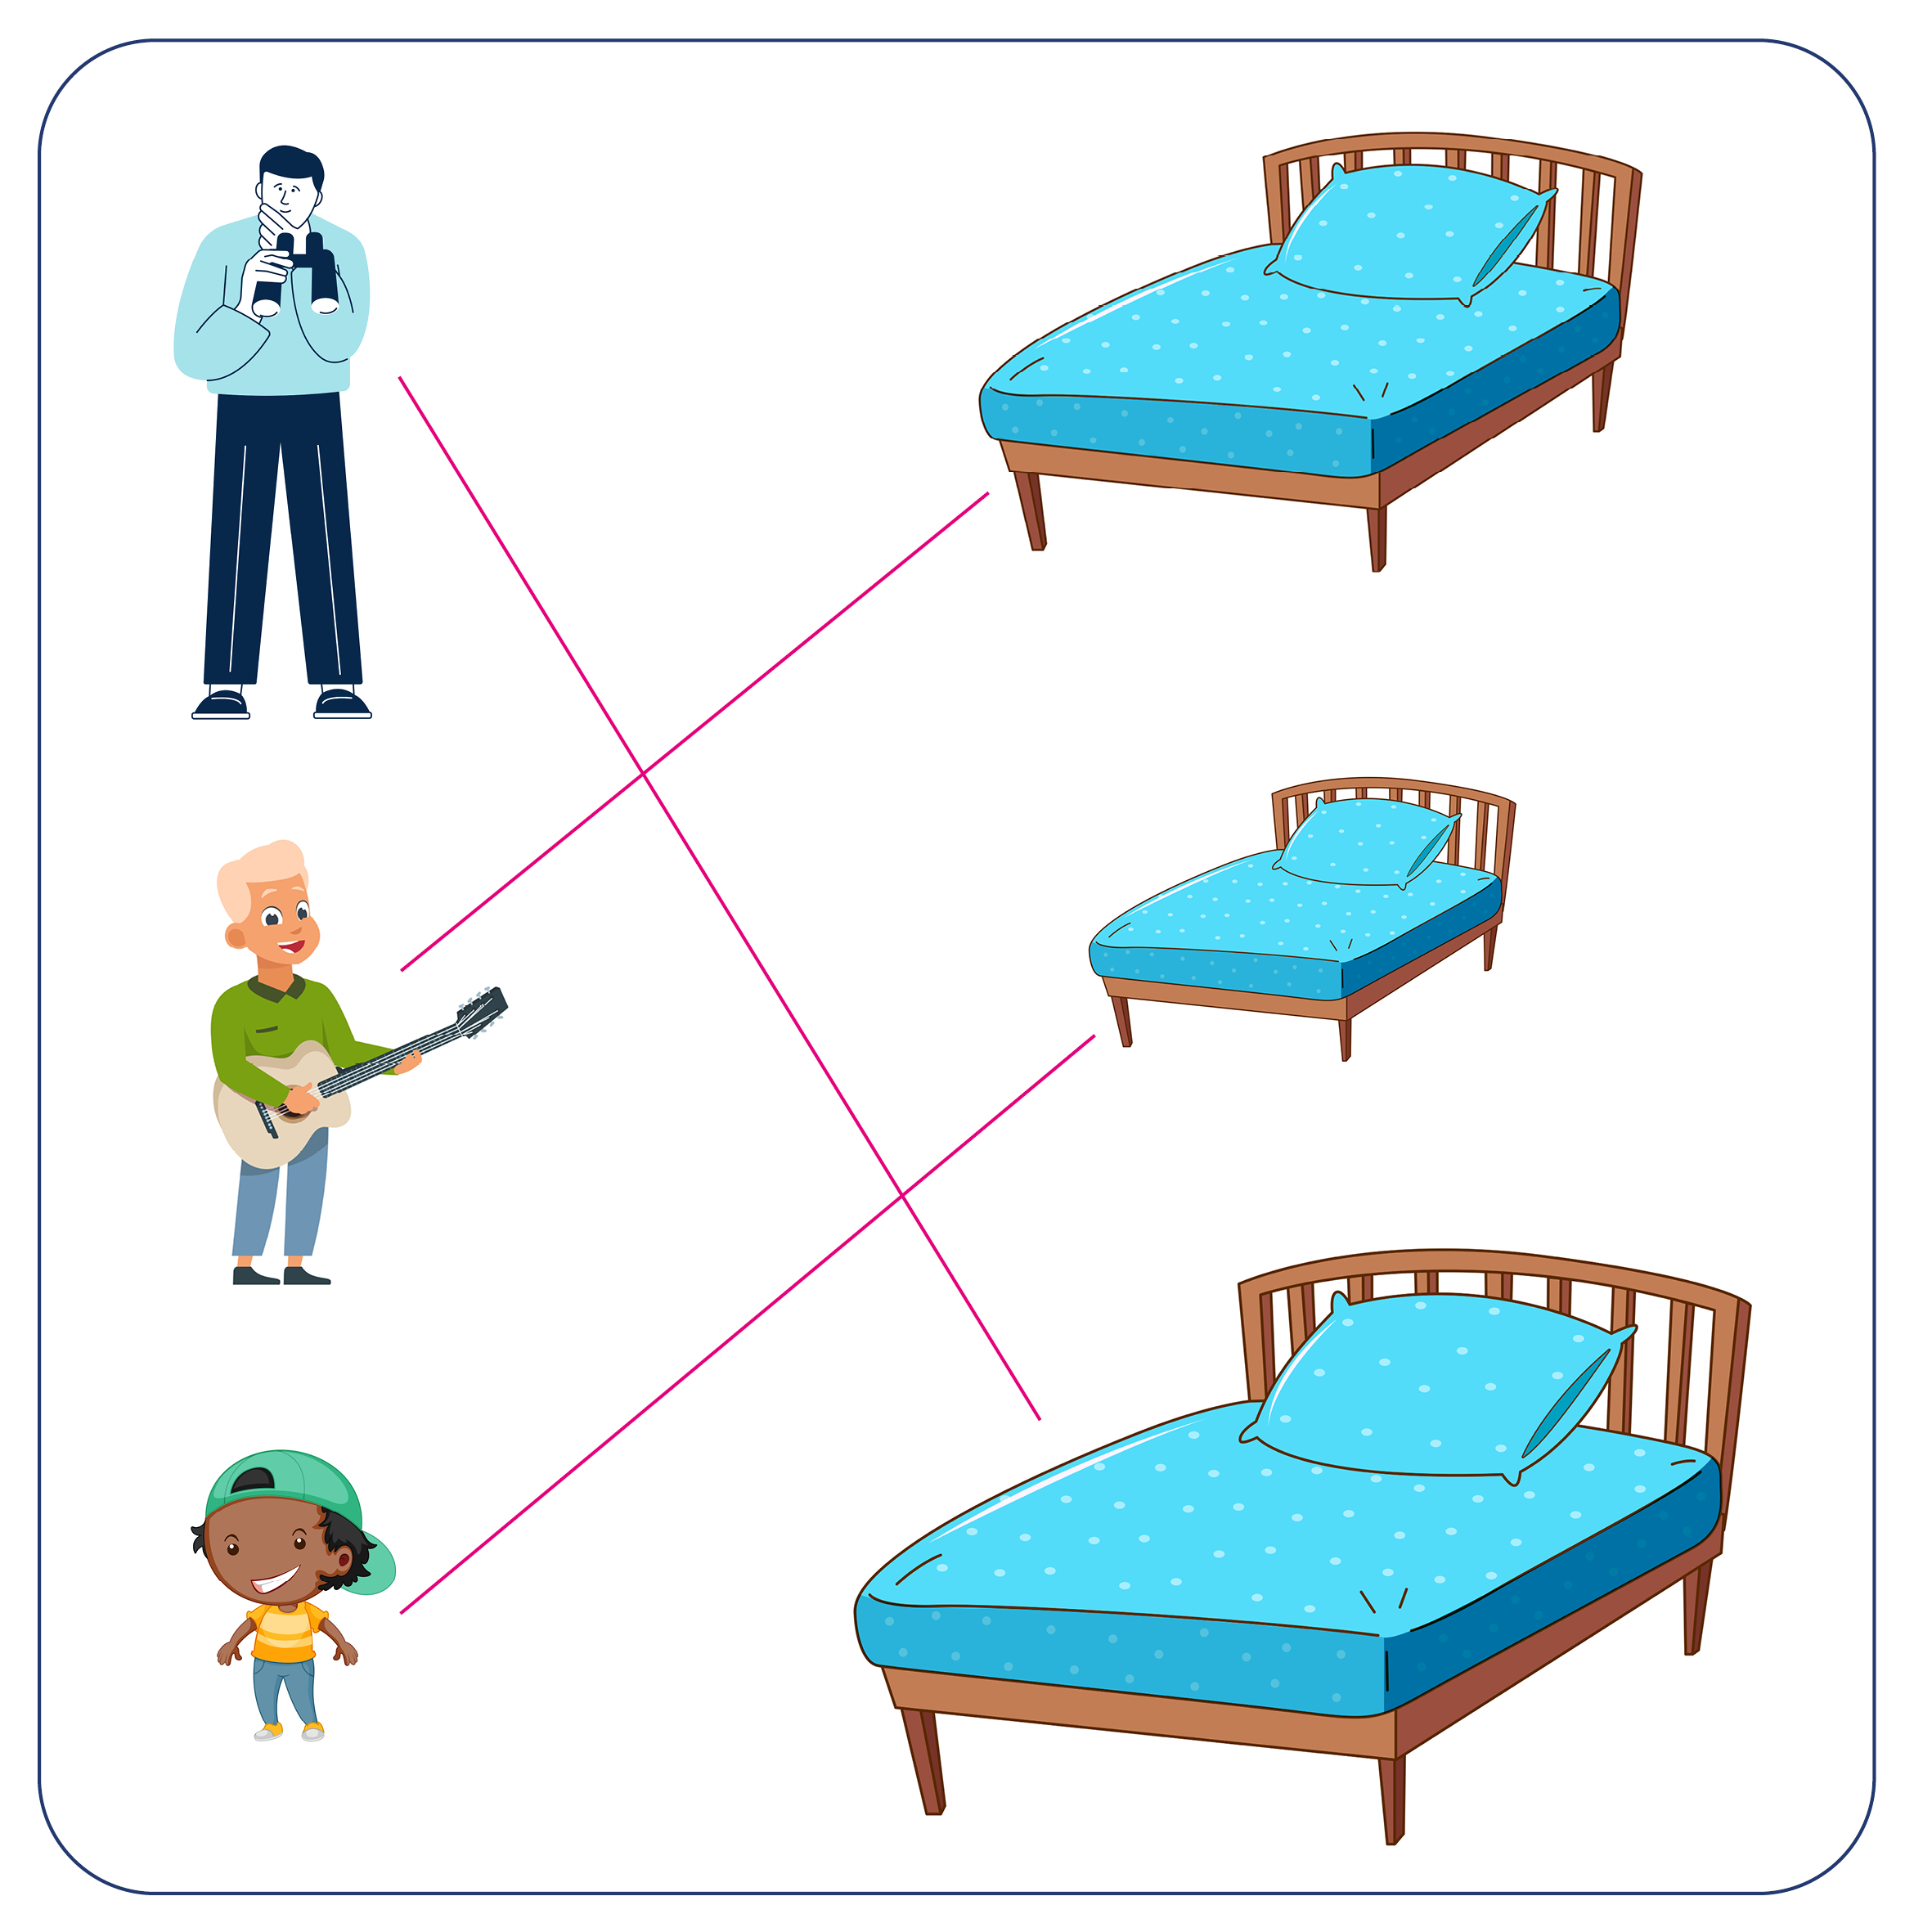
\includegraphics[width=.63\textwidth]{./media/SAEB_1ANO_MAT_FIGURA38.png}
\end{figure}

\rosa{A diferença de altura das pessoas se reflete na diferença de tamanhos das camas.}

% \num{6} PINTE COMO A JARRA MAIOR FICARIA SE FOR COLOCADO NELA TODO O LÍQUIDO DAS JARRAS MENORES.

% %\protect\hypertarget{_heading=h.gjdgxs}{}{}\textless{}Inserir a figura usando a referência: https://br.freepik.com/vetores-gratis/adesivo-de-copo-de-medicao-em-fundo-branco\_18180135.htm\#query=COPO\%20MEDIDORDESENHO\&position=2\&from\_view=search\&track=ais. Colocar as quantidades conforme o modelo a seguir.\textgreater{}

% \begin{figure}[htpb!]
% \centering
% 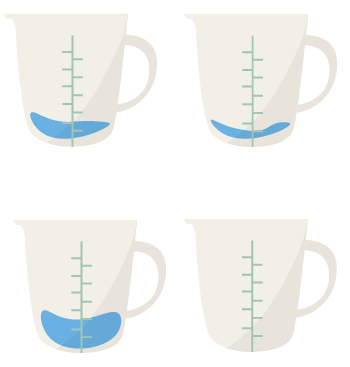
\includegraphics[width=.4\textwidth]{./media/SAEB_1ANO_MAT_FIGURA39.png}
% \end{figure}

%\coment{É importante desenvolver nos alunos uma capacidade de medição empírica, já que não existe a unidade precisa na jarra. Oriente os alunos a contarem a quantidade de riscos das jarras. Eles devem pintar até a sexta marcação.}

% \num{6} AINDA SOBRE A ATIVIDADE ANTERIOR, SE CADA MARCAÇÃO DA JARRA MAIOR MEDIR MEIO LITRO,
% QUANTOS LITROS TERIAM SIDO COLOCADOS NELA?
% \reduline{3 litros.\hfill}


% \num{6} QUAL É A CAPACIDADE TOTAL DA JARRA MAIOR DAS ATIVIDADES ANTERIORES? CONSIDERE, MAIS UMA VEZ, QUE CADA MARCAÇÃO CORRESPONDE A MEIO LITRO.
% \reduline{4 litros.\hfill}

\num{6} UTILIZE UMA RÉGUA E ESTIME O COMPRIMENTO DE CADA FIGURA A SEGUIR.

\begin{escolha}
\item \textbf{MEDIDA:} \reduline{Resposta circunstancial.\hfill}

\centering
\includegraphics[width=.6\textwidth]{./media/SAEB_1ANO_MAT_FIGURA40.png}

\vspace{1cm}

\item \textbf{MEDIDA:} \reduline{Resposta circunstancial.\hfill}

\centering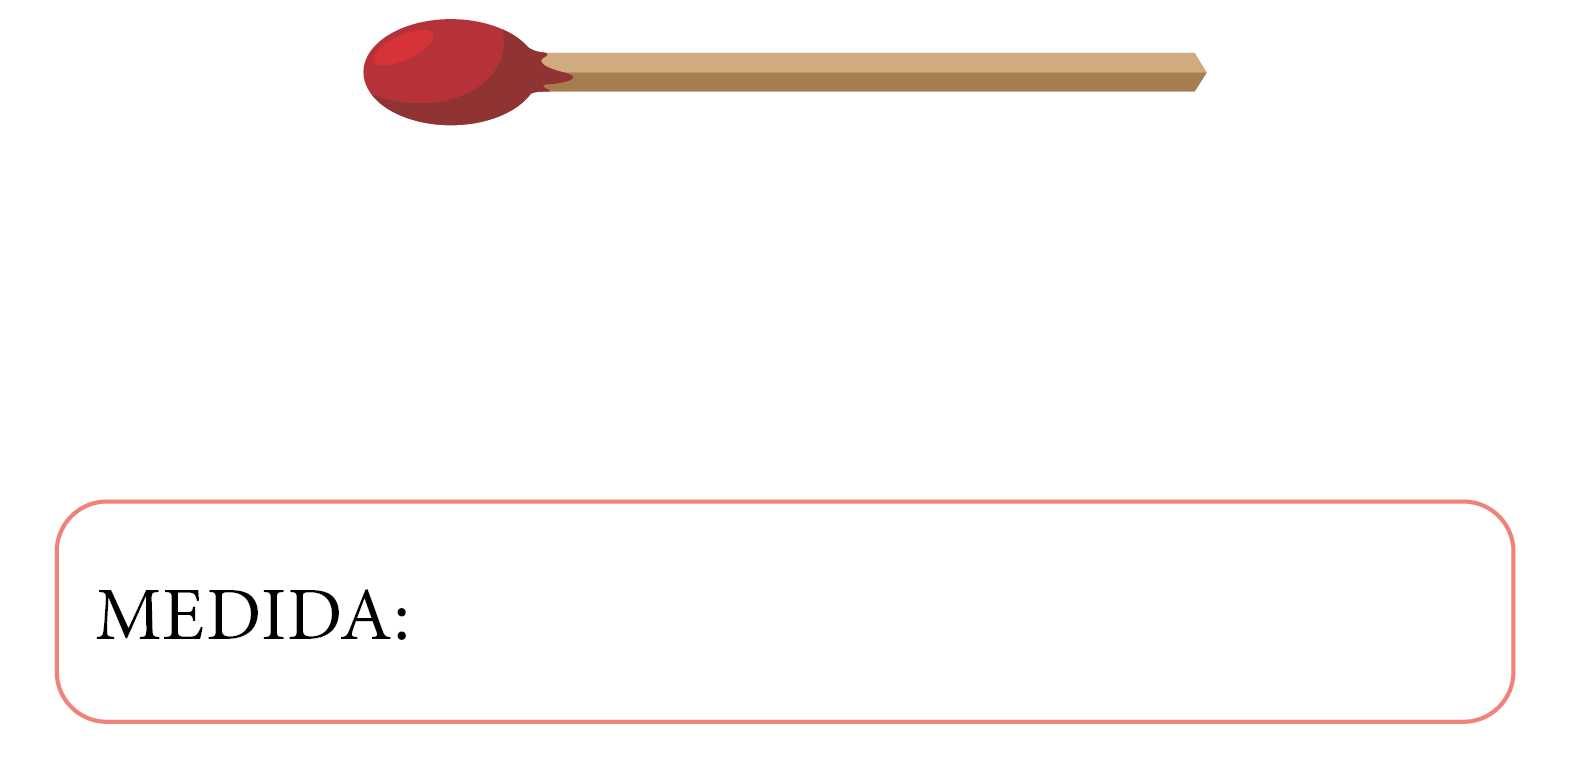
\includegraphics[width=.5\textwidth]{./media/SAEB_1ANO_MAT_FIGURA41.png}

\vspace{1cm}

\item \textbf{MEDIDA:} \reduline{Resposta circunstancial.\hfill}

\centering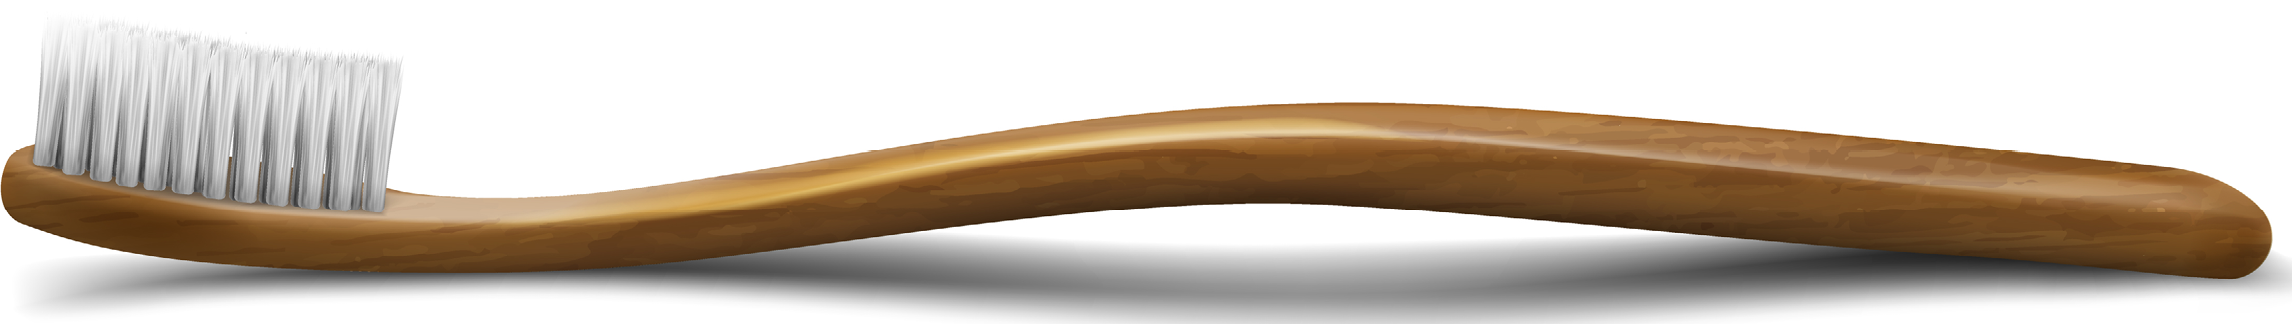
\includegraphics[width=.7\textwidth]{./media/SAEB_1ANO_MAT_FIGURA42.png}
\end{escolha}
% https://br.freepik.com/vetores-premium/icone-de-lapis-em-estilo-simples-ilustracao-vetorial-de-equipamentos-de-educacao-em-fundo-isolado-conceito-de-negocio-de-sinal-de-ferramenta-de-desenho\_30026502.htm\#%query=lapis\&position=6\&from\_view=search\&track=sph\strut
% https://br.freepik.com/vetores-premium/objetos-vetoriais-isolados-de-desenho-animado-combinam-e-fogo\_29291308.htm\#query=palito\%20de\%20f\%C3\%B3sforo\%20desenho\&position=9\&from\_view=search\&track=ais\%strut
% https://br.freepik.com/vetores-premium/objetos-vetoriais-isolados-de-desenho-animado-combinam-e-fogo\_29291308.htm\#query=palito\%20de\%20f\%C3\%B3sforo\%20desenho\&position=9\&from\_view=search\&track=ais\%strut

%\coment{Oriente os alunos quanto ao fato de suas réguas medirem comprimentos menores do que um metro. Explique que o centímetro é uma subdivisão dessa unidade de medida. Este não é o momento de quantificar essa subdivisão. Basta que entendam que se trata de outra unidade para medir comprimentos.}

\section*{TREINO}

\num{1} COMPARE AS ALTURAS DAS CRIANÇAS REPRESENTADAS A SEGUIR.

%\textless{} https://br.freepik.com/vetores-gratis/quatro-criancas\_4906544.htm\#page=2\&query=crian\%C3\%A7as\%20com\%20diferentes\%20alturas\%20desenho\&position=13\&from\_view=search\&track=ais.\textgreater{}

\begin{figure}[H]
\centering
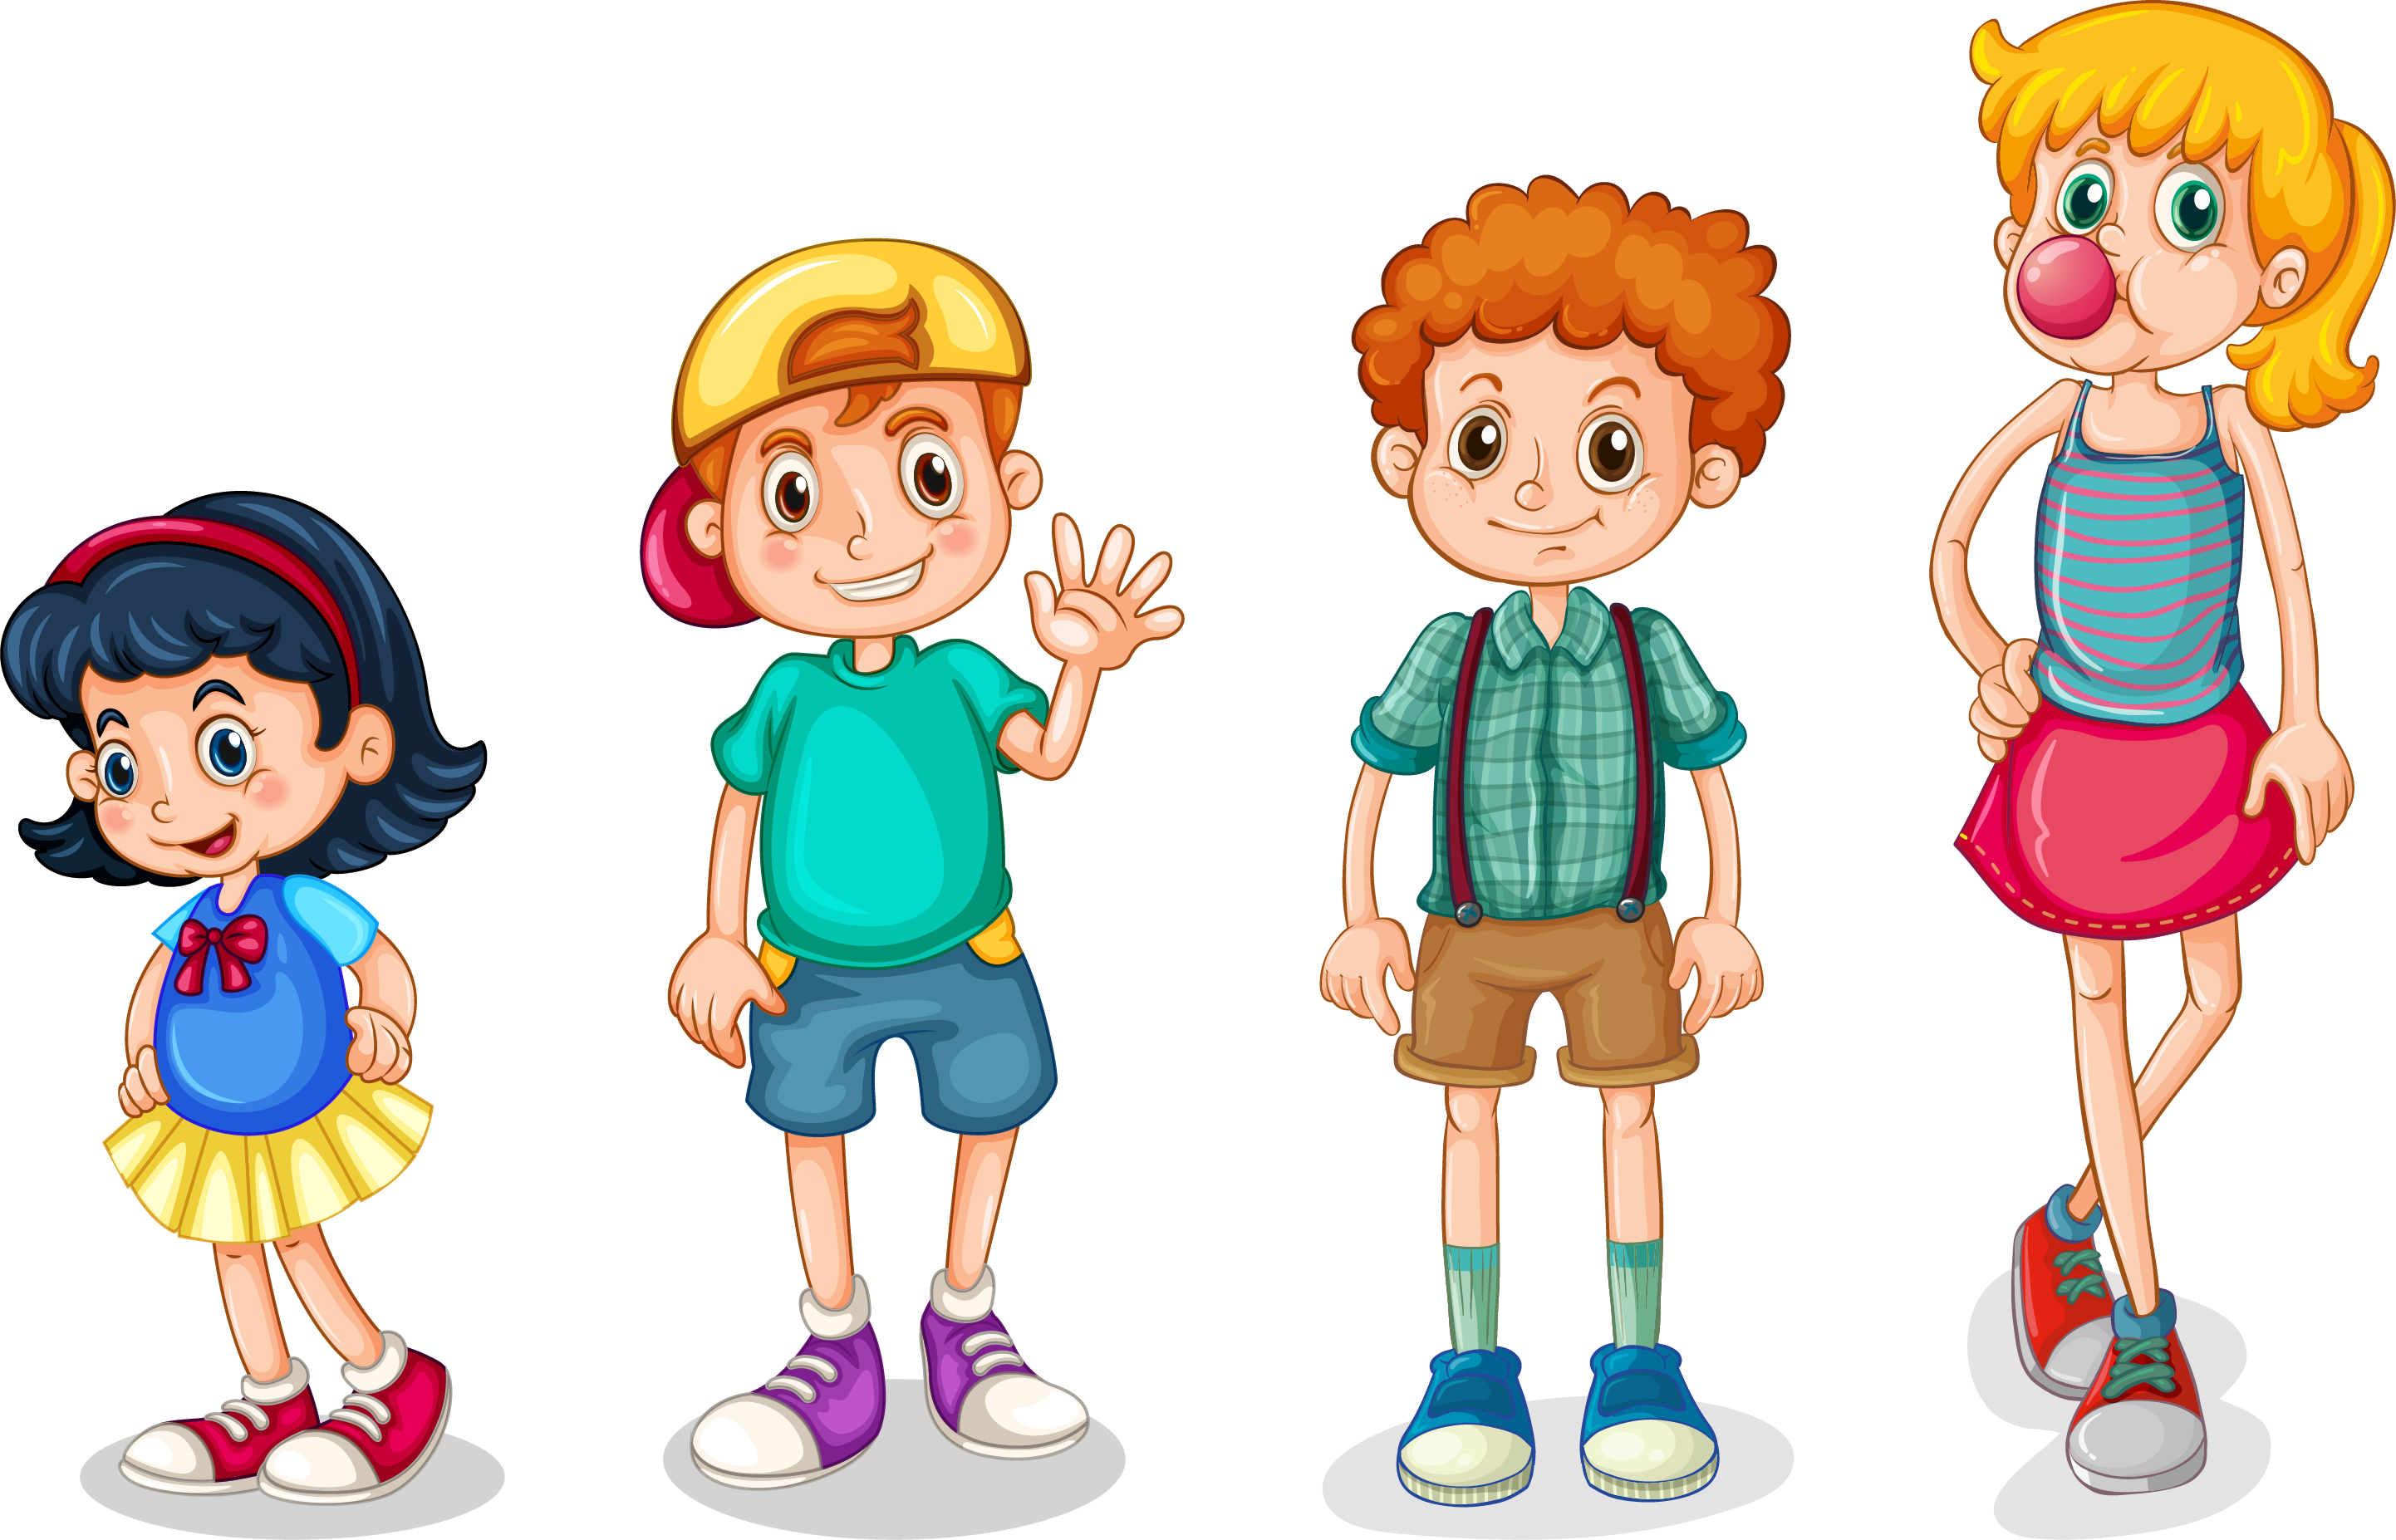
\includegraphics[width=.6\textwidth]{./media/SAEB_1ANO_MAT_FIGURA43.png}
\end{figure}

A CRIANÇA MAIS ALTA É

\begin{escolha}[itemsep=-5pt]
\item A MENINA DE SAIA AMARELA.

\item A MENINA MASCANDO CHICLETE.

\item O MENINO DE BONÉ.

\item O MENINO DE TÊNIS AZUL.
\end{escolha}

\num{2} OBSERVE A IMAGEM A SEGUIR.

\begin{figure}[H]
\centering
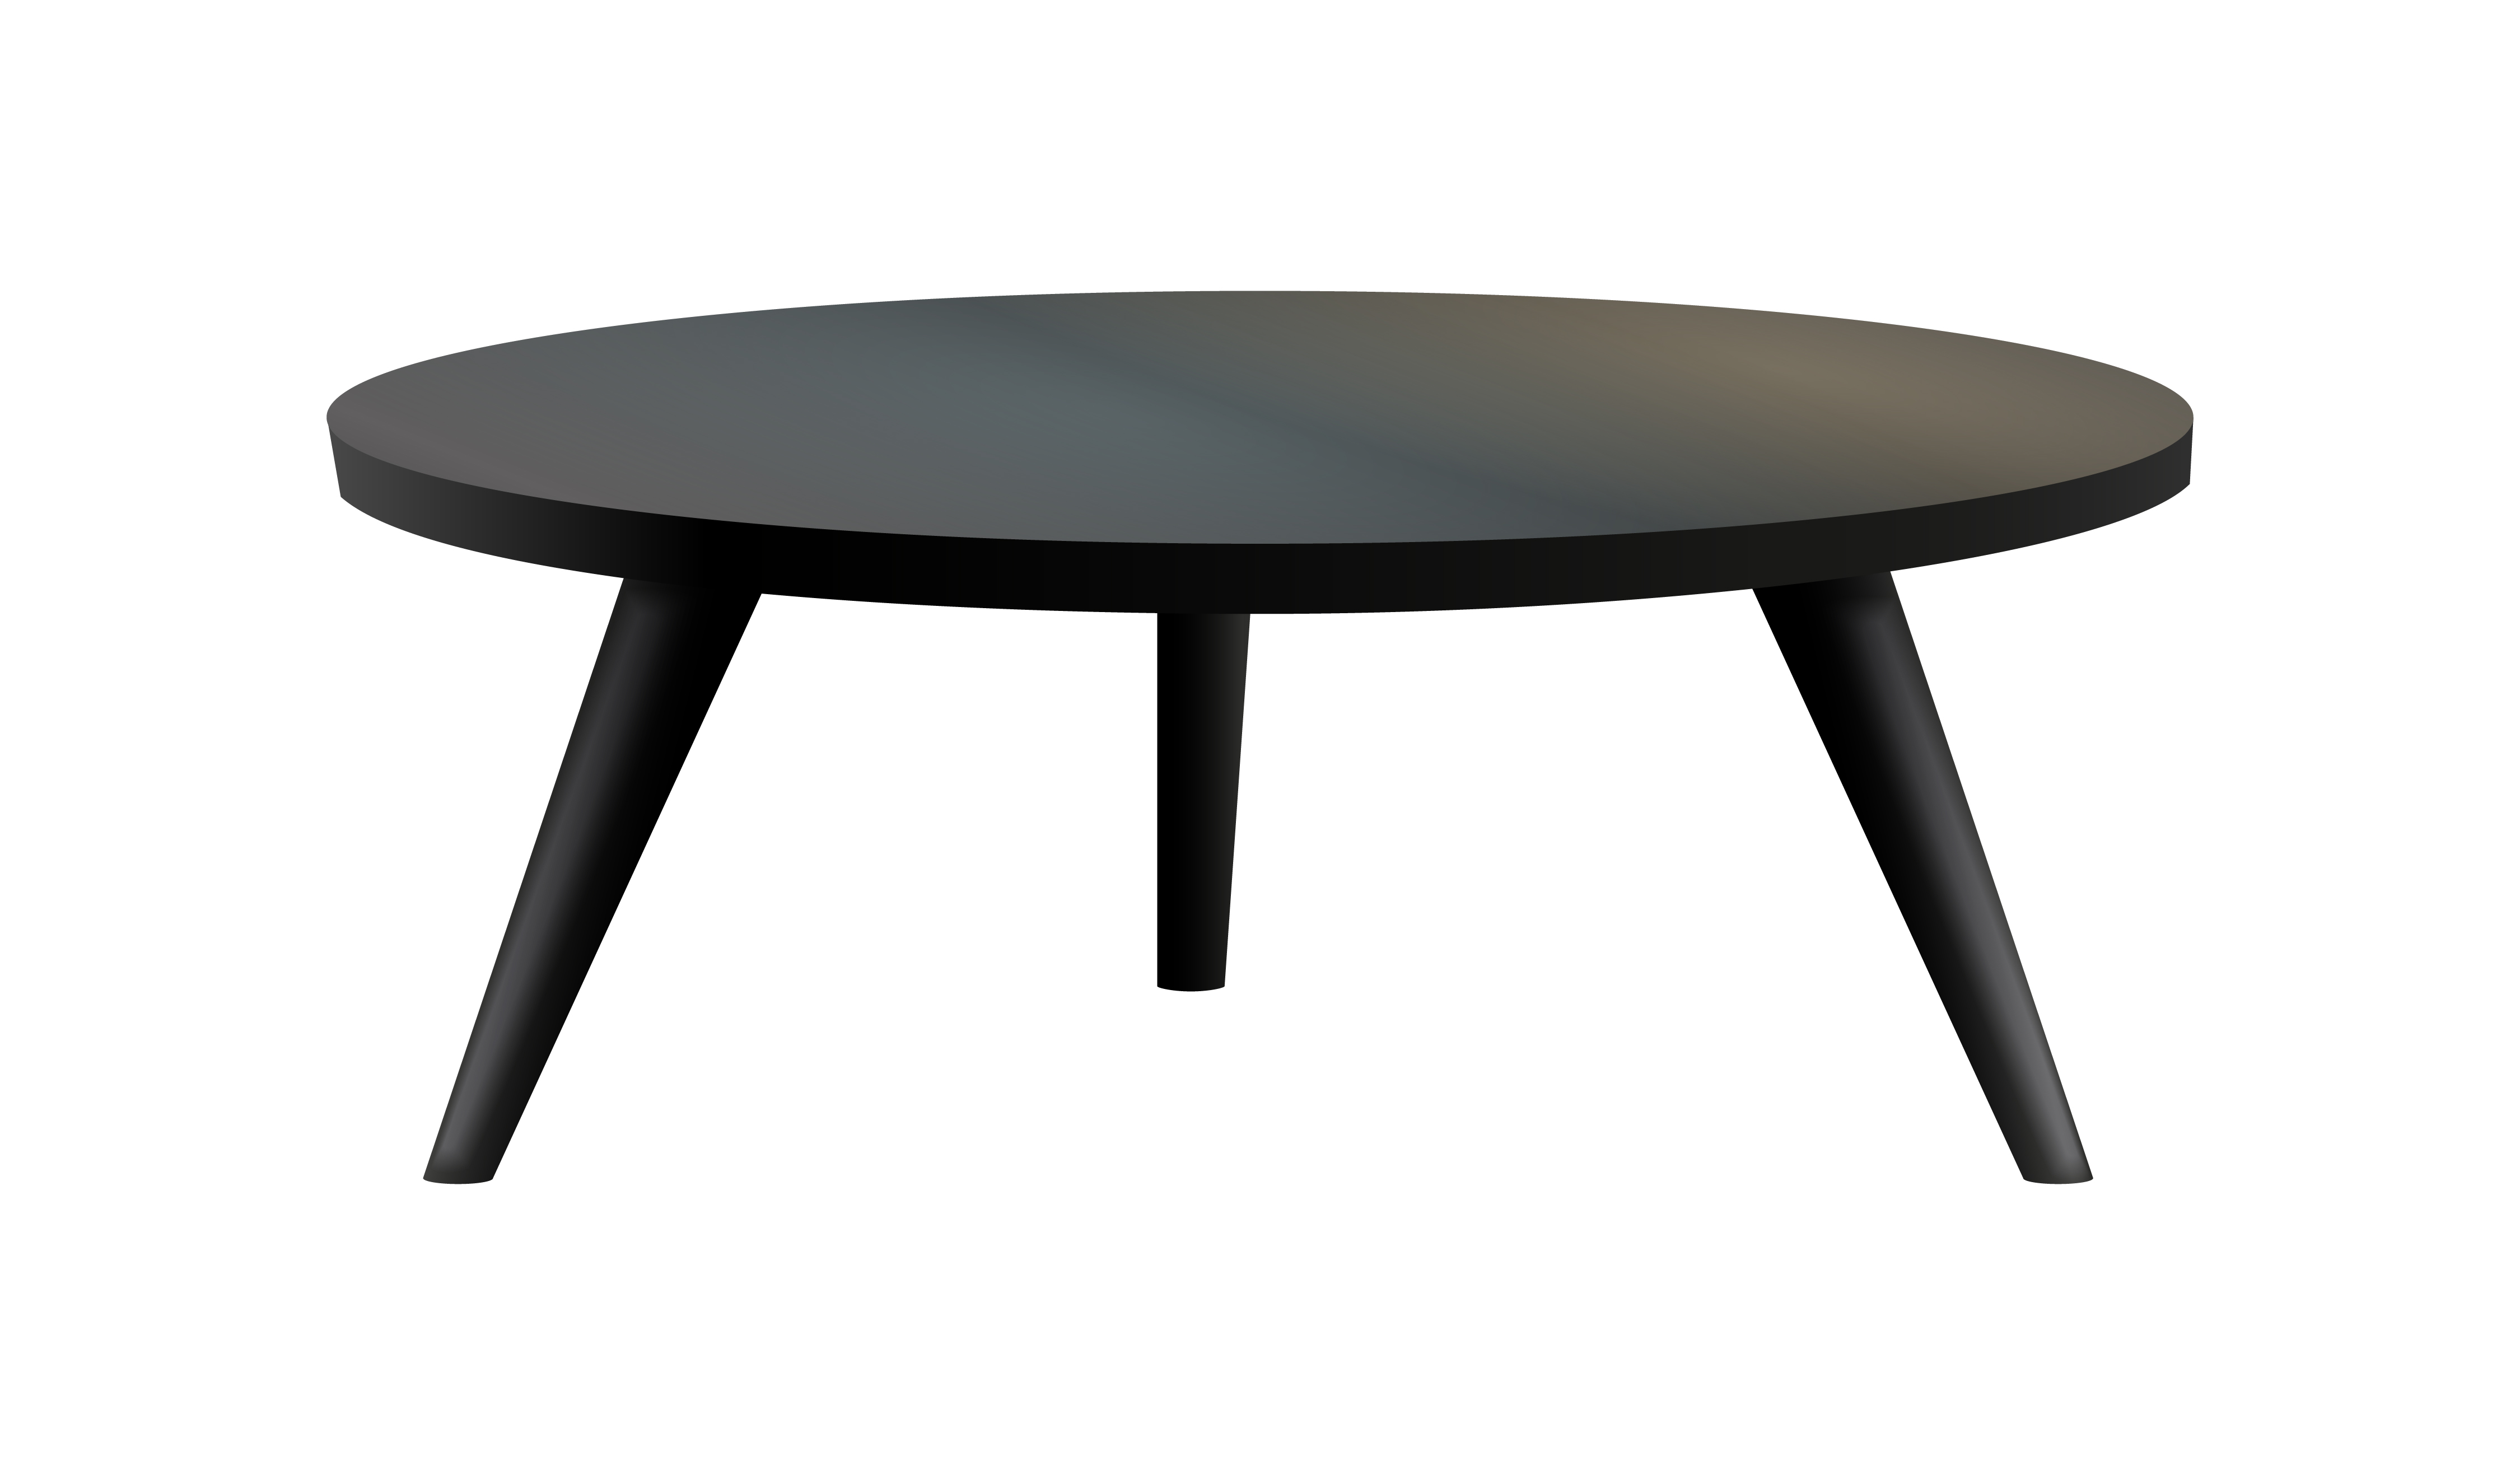
\includegraphics[width=.4\textwidth]{media/image32b.jpg}
\end{figure}

QUAL DESTES É O MELHOR INSTRUMENTO PARA SE MEDIR A DISTÂNCIA DO TAMPO DA MESA ATÉ O CHÃO?

\begin{multicols}{2}
\begin{escolha}[itemsep=-5pt]
\item UMA BALANÇA.

\item UM COPO DE MEDIÇÃO.

\item UMA RÉGUA.

\item UMA PANELA.
\end{escolha}
\end{multicols}

\num{3} VEJA A IMAGEM, EM QUE SE MOSTRA A MASSA DE JULIANA.

%\textless{}https://br.freepik.com/fotos-gratis/closeup-de-peso-escalas-conceito-de-excesso-de-peso-e-obesidade\_3219089.htm\#page=5\&query=regua\%20medindo\&position=49\&from\_view=search\&track=ais\textgreater{}

\begin{figure}[htpb!]
\centering
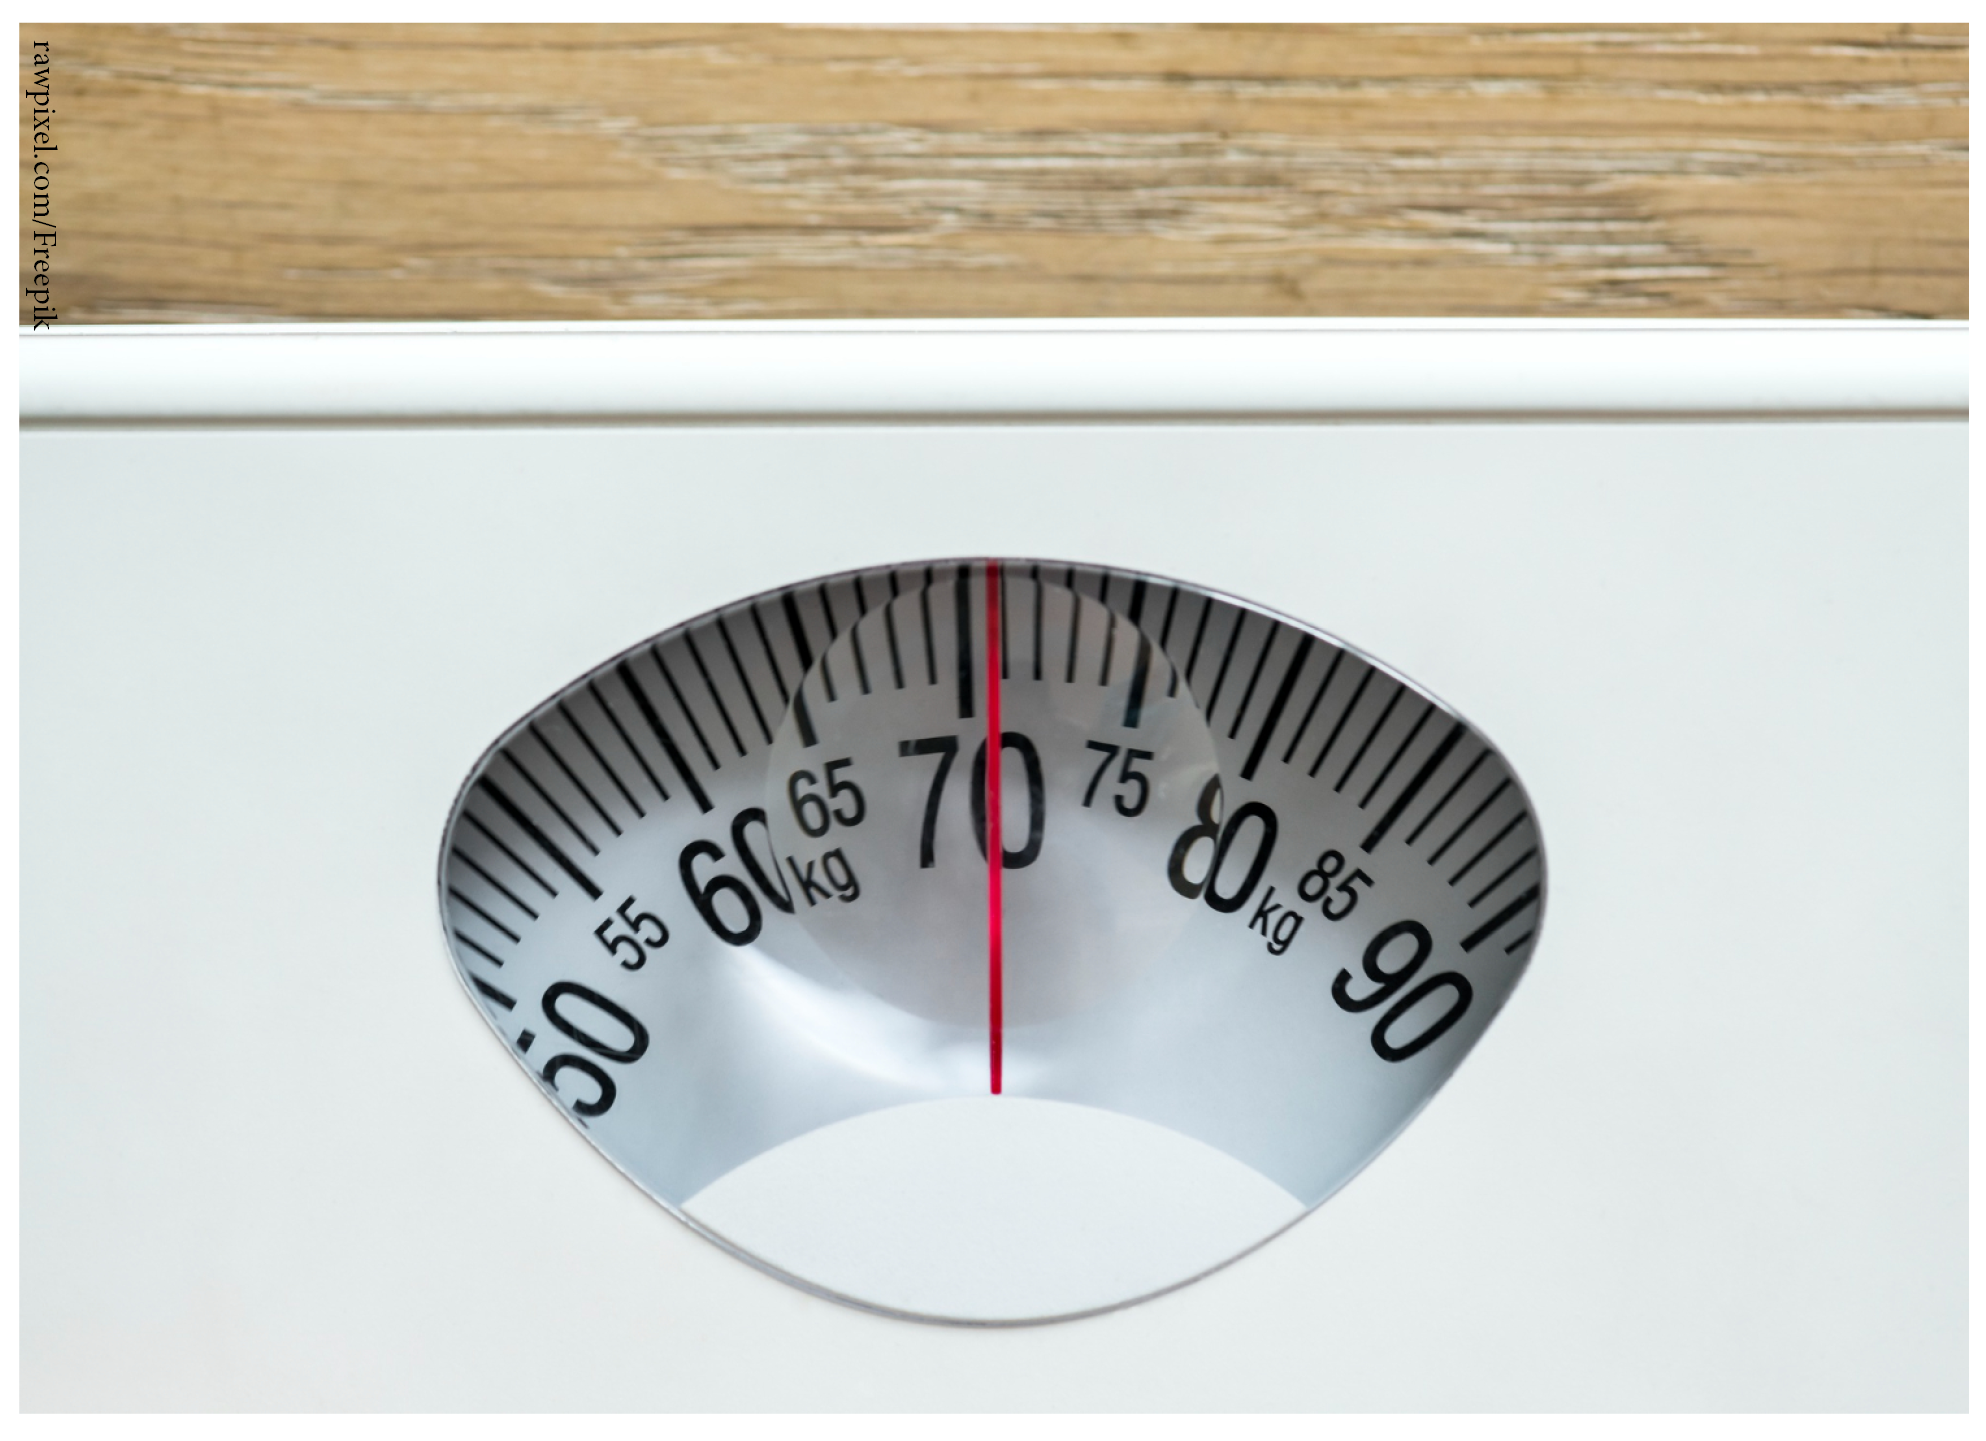
\includegraphics[width=3.03770in,height=1.48580in]{./media/SAEB_1ANO_MAT_FIGURA44.png}
\end{figure}

QUAL É A MASSA DE JULIANA, MEDIDA EM QUILOGRAMAS?

\begin{multicols}{2}
\begin{escolha}[itemsep=-5pt]
\item 69.

\item 70.

\item 71.

\item 72.
\end{escolha}
\end{multicols}

\chapter[{EM QUE DIA DA SEMANA CAI MEU ANIVERSÁRIO?}]{\large EM QUE DIA DA SEMANA CAI MEU ANIVERSÁRIO?}
\markboth{Módulo 4}{}

%\coment{Neste módulo, vamos desenvolver nos alunos a habilidade de orientar-se no tempo, sabendo identificar o tempo presente, assim como prever dias e horários de eventos futuros.}

\section*{HABILIDADES DO SAEB}

\begin{itemize}
\item \uppercase{Identificar sequência de acontecimentos relativos a um dia.}
\item \uppercase{Identificar datas, dias da semana ou meses do ano em calendário ou
escrever uma data, apresentando o dia, o mês e o ano.}
\item \uppercase{Determinar a data de início, a data de término ou a duração de um
acontecimento entre duas datas.}
\item \uppercase{Determinar o horário de início, o horário de término ou a duração de
um acontecimento.}
\end{itemize}

\subsection{Habilidades da BNCC}

\begin{itemize}\enlargethispage{2\baselineskip}
\item EF01MA16, EF01MA17, EF01MA18.
\end{itemize}

\conteudo{É COMUM AS PESSOAS FICAREM ANSIOSAS PARA CHEGAR O DIA DO PRÓPRIO ANIVERSÁRIO.
NÃO VEMOS A HORA DE GANHAR PRESENTES, COMER BOLO, ASSOPRAR A VELA E
FICAR COM OS AMIGOS, NÃO É MESMO?

NO SEU CASO ESPECÍFICO, VOCÊ SABE EM QUE DIA ISSO ACONTECERÁ? EM QUE DIA
DA SEMANA ISSO VAI CAIR? SE VOCÊ VAI TER UMA FESTA DE ANIVERSÁRIO, VOCÊ SABE DIZER A 
QUE HORAS ELA VAI COMEÇAR OU TERMINAR? 

\begin{center}
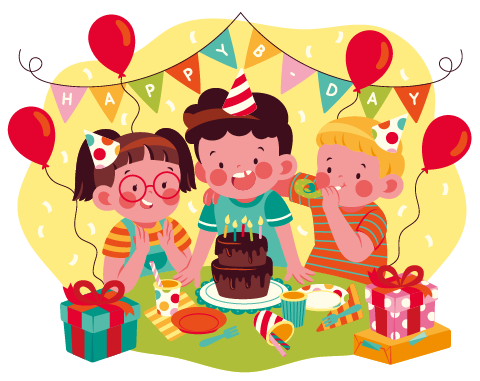
\includegraphics[width=.9\textwidth]{./media/SAEB_1ANO_MAT_FIGURA45.png}
\end{center}

VAMOS LEMBRAR COMO É ORGANIZADO NOSSO CALENDÁRIO.

O ANO É DIVIDIDO EM 365 DIAS, E CADA DIA TEM 24 HORAS. ALÉM DISSO, O ANO
TAMBÉM É DIVIDIDO EM 12 MESES, E OS MESES TÊM ENTRE 28 E 31 DIAS. VOCÊ LEMBRA O NOME DOS MESES E A QUANTIDADE
DE DIAS DE CADA UM? OBSERVE:

\noindent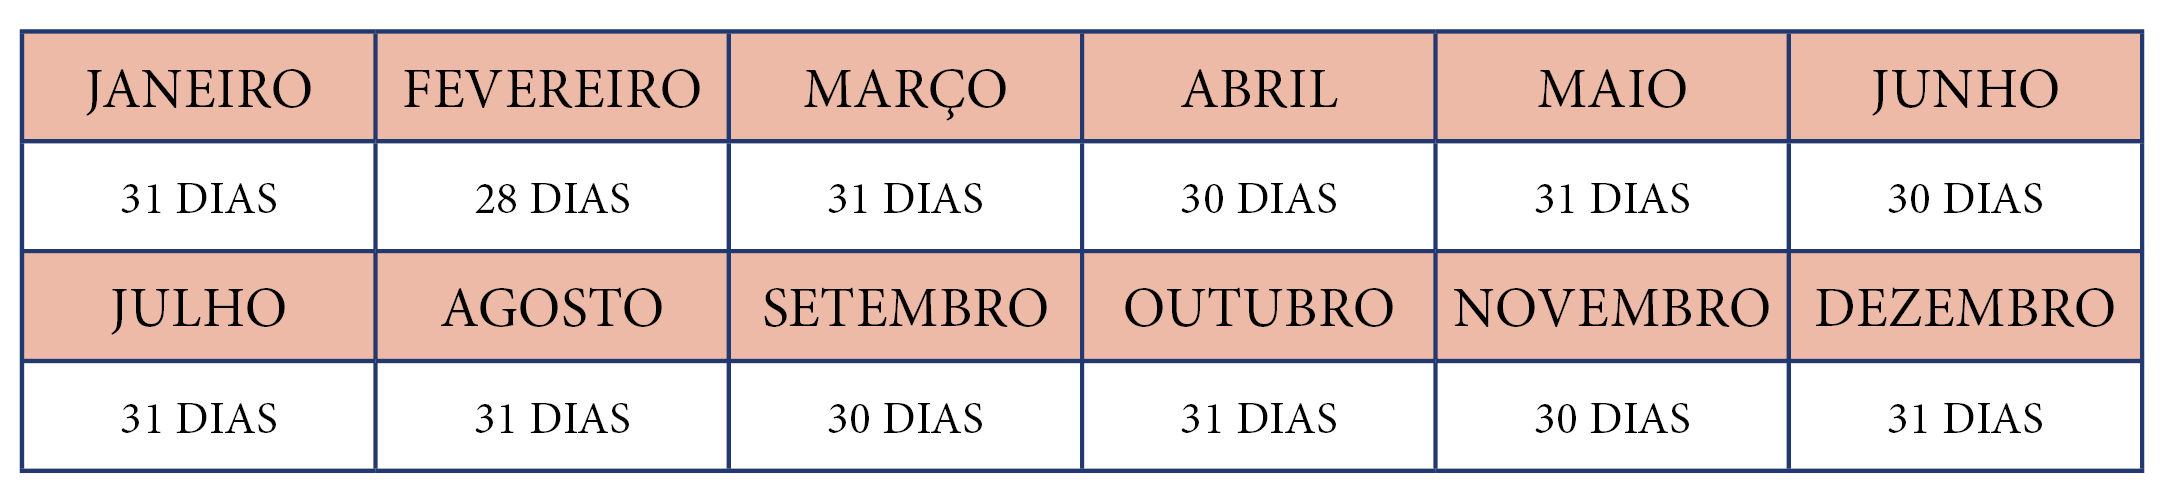
\includegraphics[width=\textwidth]{./media/SAEB_1ANO_MAT_FIGURA46.png}

OS MESES ESTÃO ORGANIZADOS EM SEMANAS, QUE SÃO DIVIDIDAS EM 7 DIAS. OBSERVE OS NOMES
DESSES DIAS: DOMINGO --- SEGUNDA-FEIRA --- TERÇA-FEIRA --- QUARTA-FEIRA --- QUINTA-FEIRA 
--- SEXTA-FEIRA --- SÁBADO.
}

\pagebreak
\section*{ATIVIDADES}

\num{1} VAMOS DESCOBRIR QUE DIA É HOJE? ESCREVA O QUE SE PEDE A SEGUIR.

\begin{escolha}
\item EM QUE ANO ESTAMOS?

\reduline{Resposta circunstancial.\hfill}

\item EM QUE MÊS ESTAMOS?

\reduline{Resposta circunstancial.\hfill}

\item QUE DIA DO MÊS É HOJE?

\reduline{Resposta circunstancial.\hfill}

\item QUE DIA DA SEMANA É HOJE?

\reduline{Resposta circunstancial.\hfill}

\item QUE HORAS SÃO NESTE MOMENTO EM QUE VOCÊ ESTÁ RESOLVENDO ESTA ATIVIDADE?

\reduline{Resposta circunstancial.\hfill}
\end{escolha}

% \begin{figure}[htpb!]
% \centering
% 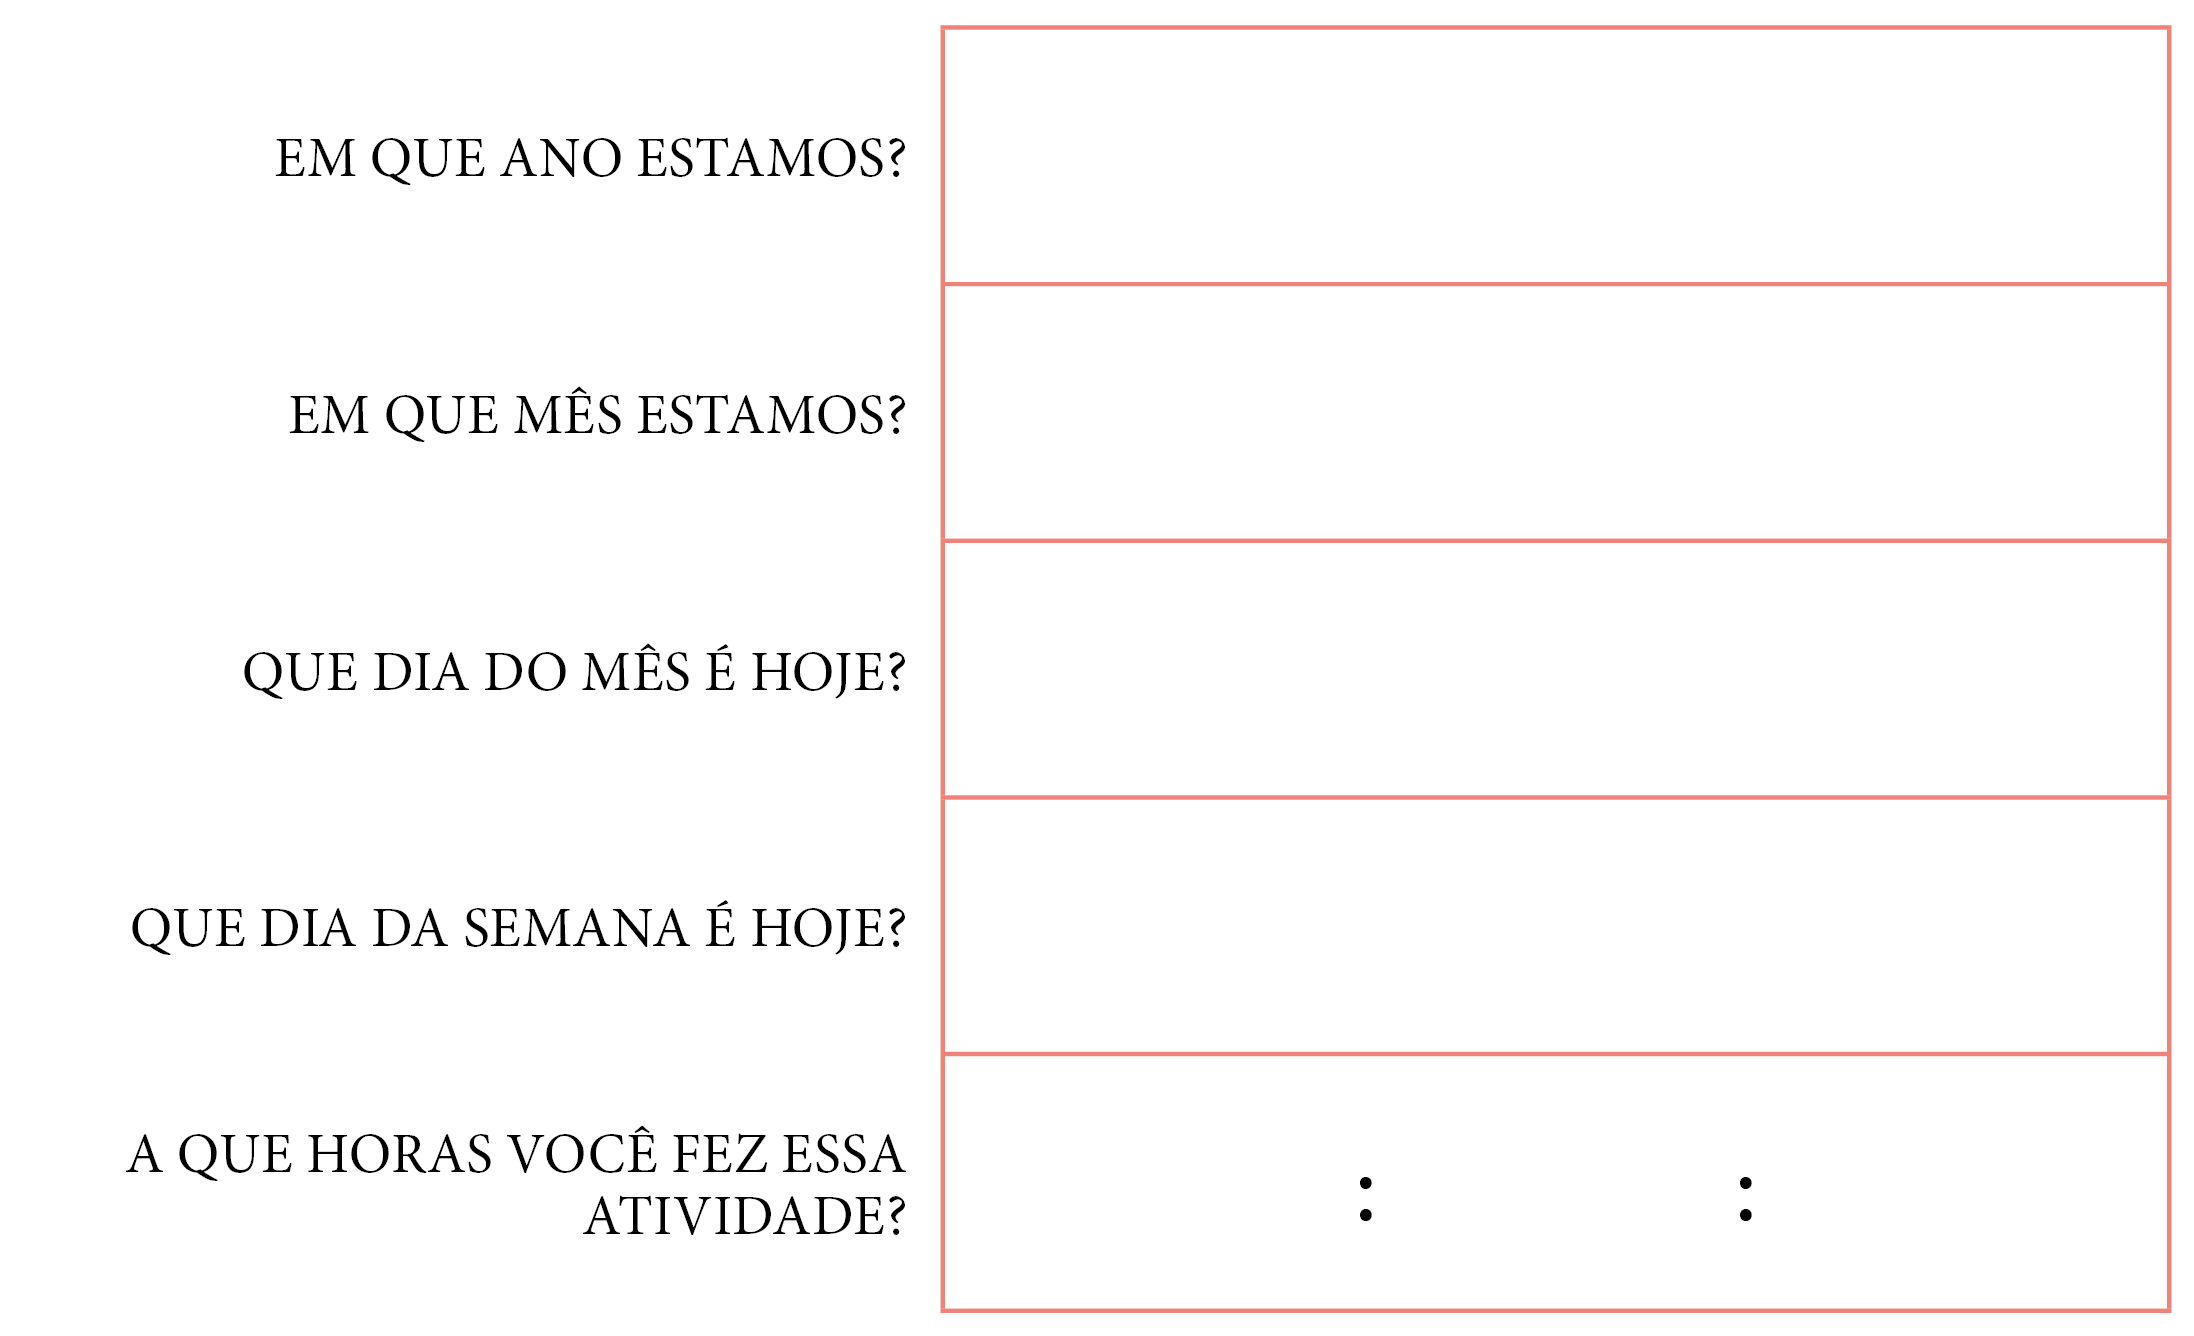
\includegraphics[width=\textwidth]{./media/SAEB_1ANO_MAT_FIGURA48.png}
% \end{figure}

%\coment{O mais importante nesta atividade é fazer com que o aluno consiga diferenciar cada classificação do tempo, como saber diferenciar dia do mês e dia da semana, por exemplo. Oriente-os a preencherem o horário com horas, minutos e segundos. Essa atividade pode e deve ser usada com fins de avaliação diagnóstica.}

\num{2} PINTE OS QUADRADOS COM A COR EQUIVALENTE.

\begin{figure}[htpb!]
\centering
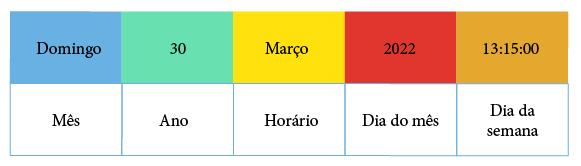
\includegraphics[width=\textwidth]{./media/SAEB_1ANO_MAT_FIGURA49.png}
\end{figure}

\rosa{A sequência de cores é: amarelo, vermelho, laranja, verde e azul.}

\num{3} CIRCULE NO CALENDÁRIO O DIA DO SEU ANIVERSÁRIO E ANOTE EM QUE DIA DA SEMANA ELE ESTÁ.

%\textless{} https://br.freepik.com/vetores-premium/calendario-de-cores-para-2023-com-um-coelho-de-personagem-fofo-a-semana-comeca-no-domingo-diversao-e-estilo-de-desenho-animado-de-design-brilhante\_34560382.htm\#query=calend\%C3\%A1rio\%20infantil\%202023\%20em\%20portugu\%C3\%AAs\&position=6\&from\_view=search\&track=ais. Traduzir os nomes dos meses, além das iniciais dos dias da semana.\textgreater{} 

\begin{figure}[H]
\centering
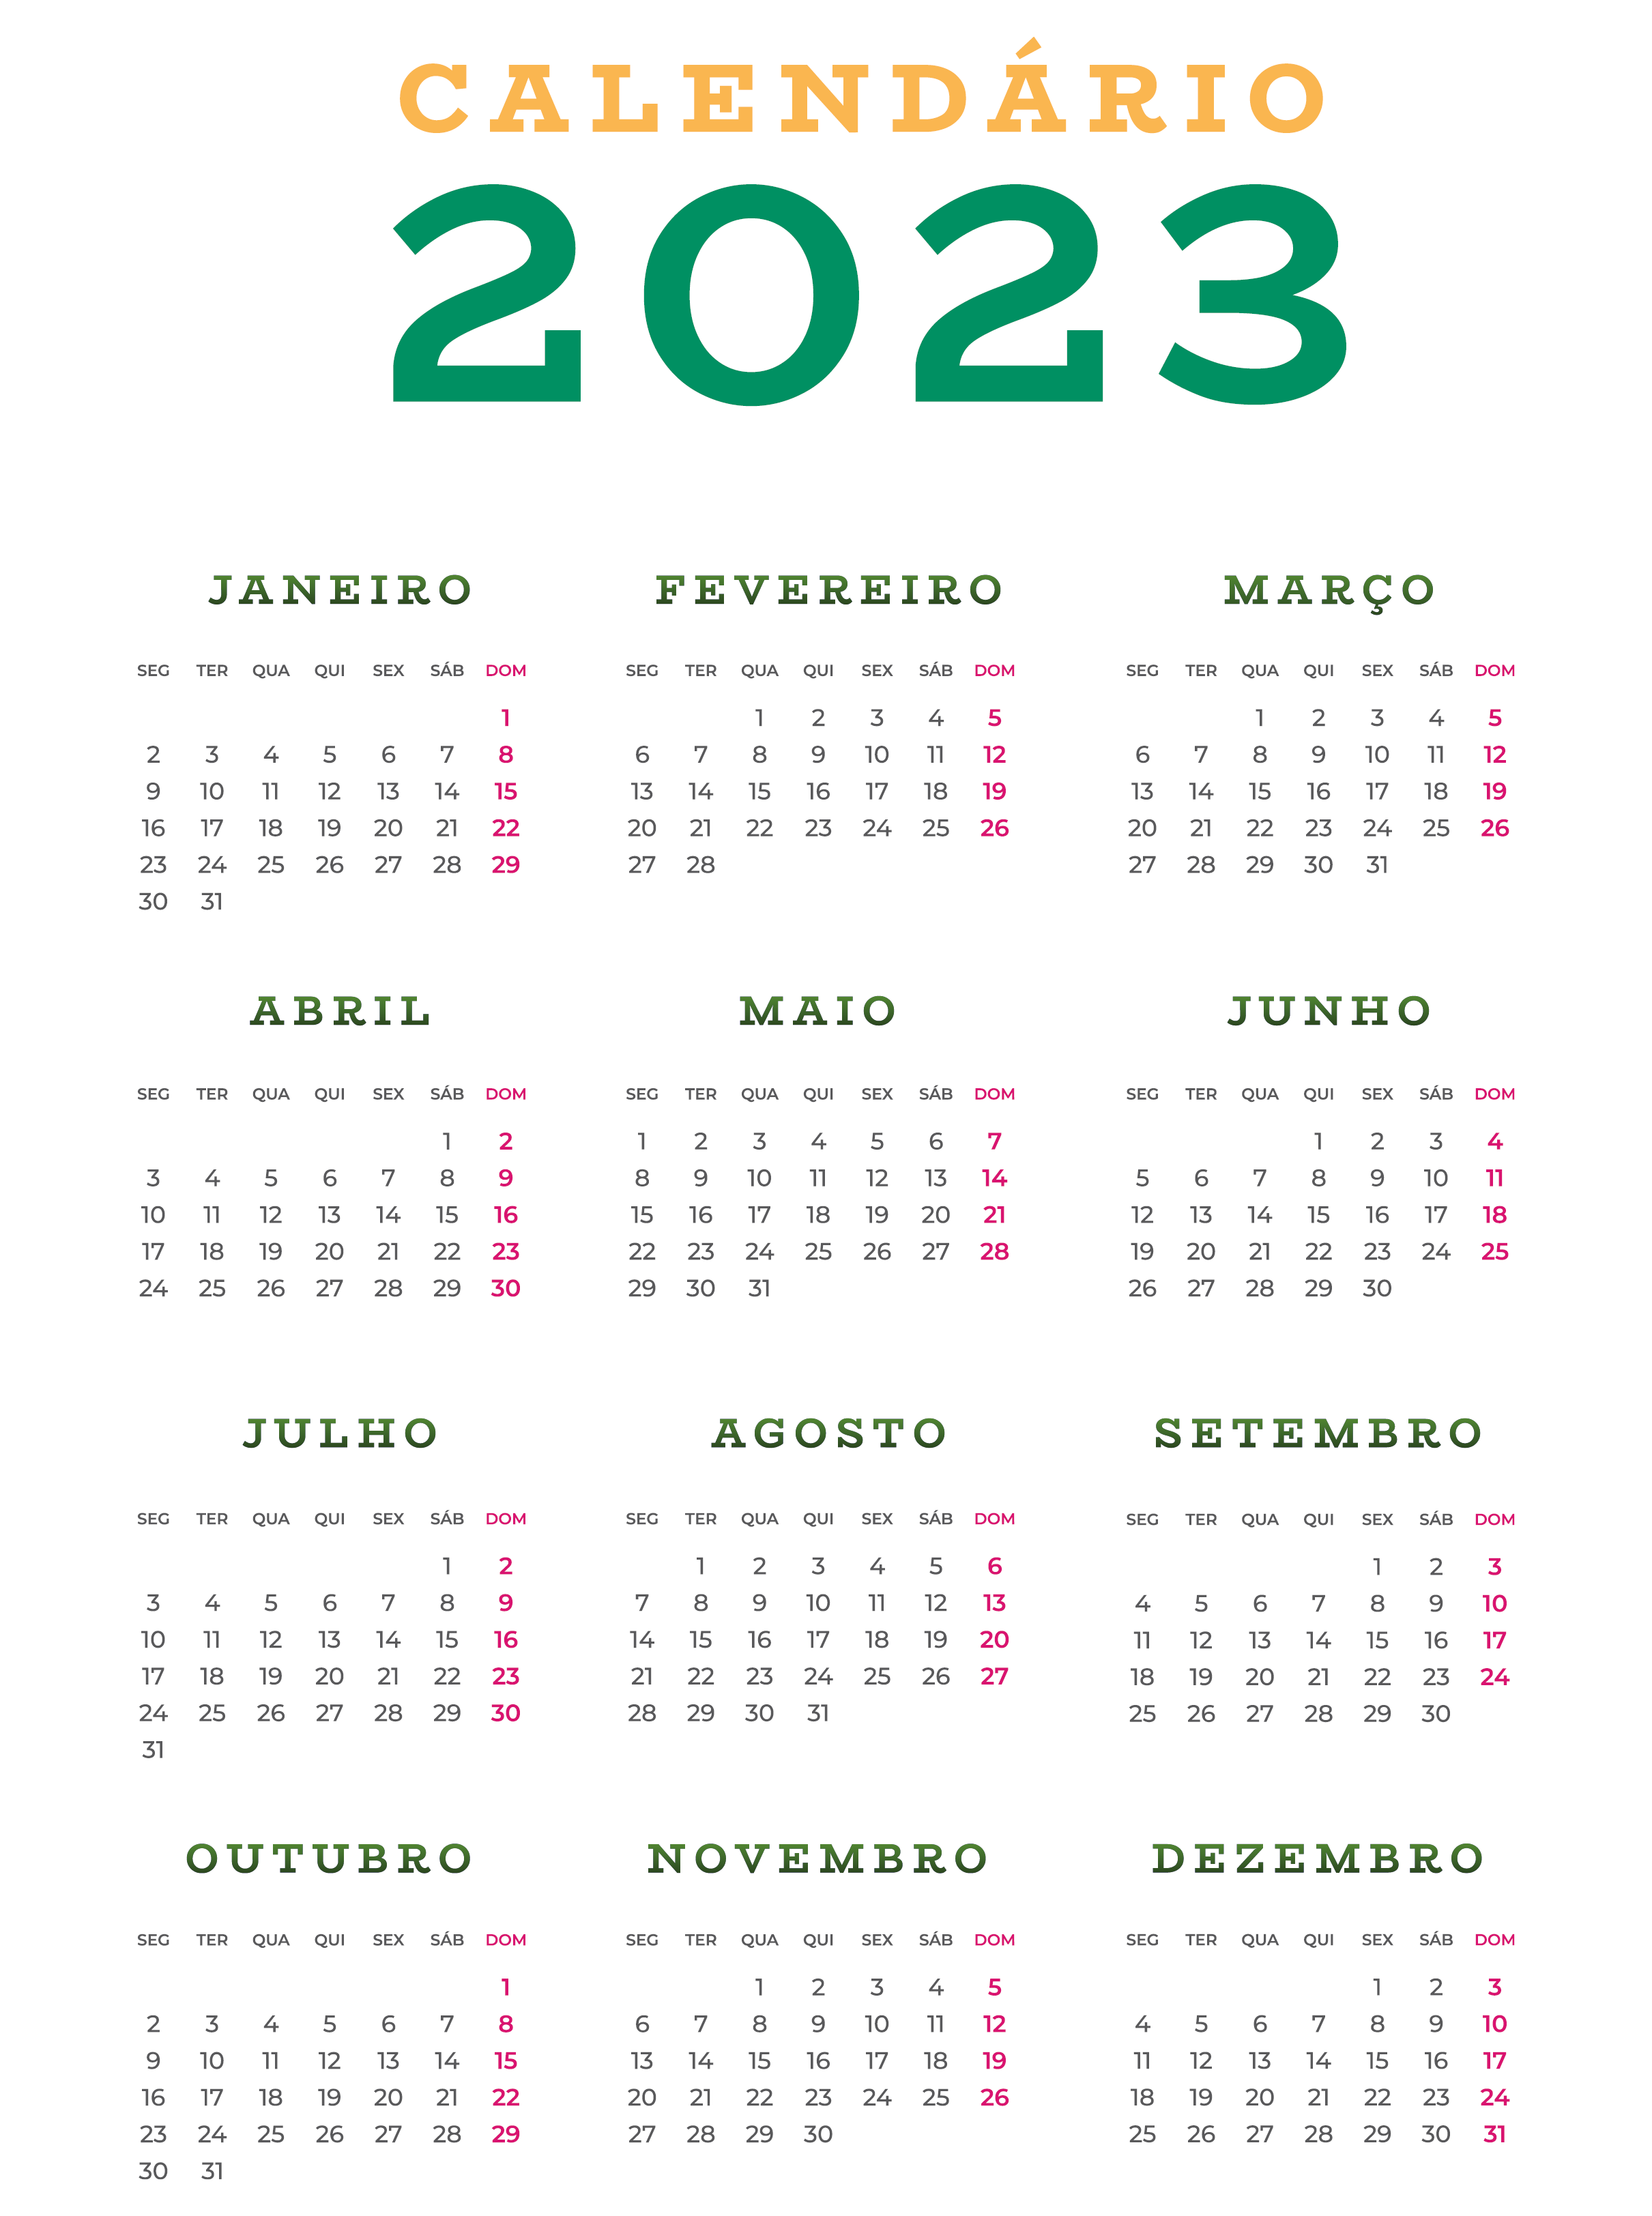
\includegraphics[width=\textwidth]{./media/SAEB_1ANO_MAT_FIGURA51.png}
\end{figure}


\num{4} ANALISE AS FIGURAS E LISTE A ORDEM DOS ACONTECIMENTOS EM UM DIA.

%\textless{}Inserir as figuras na ordem do modelo a seguir. Utilizar as referências: https://br.freepik.com/vetores-premium/garoto-bonito-comendo-delicioso-arroz-frito\_35549113.htm\#query=crian\%C3\%A7a\%20almo\%C3\%A7ando\&position=48\&from\_view=search\&track=ais; https://br.freepik.com/vetores-gratis/menino-dormir-cama\_4388324.htm\#query=crian\%C3\%A7a\%20acordando\&position=21\&from\_view=search\&track=ais; https://br.freepik.com/vetores-gratis/menino-que-dorme-na-cama\_1021842.htm\#query=crian\%C3\%A7a\%20acordando\&position=23\&from\_view=search\&track=ais; https://br.freepik.com/vetores-gratis/uma-garota-fazendo-o-exame\_2607446.htm\#query=crian\%C3\%A7a\%20estudasndo\&position=0\&from\_view=search\&track=ais e https://br.freepik.com/vetores-gratis/criancas-felizes-brincando-com-brinquedos\_11575551.htm\#query=crian\%C3\%A7a\%20brincando\&position=32\&from\_view=search\&track=ais \textgreater{}

\begin{figure}[H]
\centering
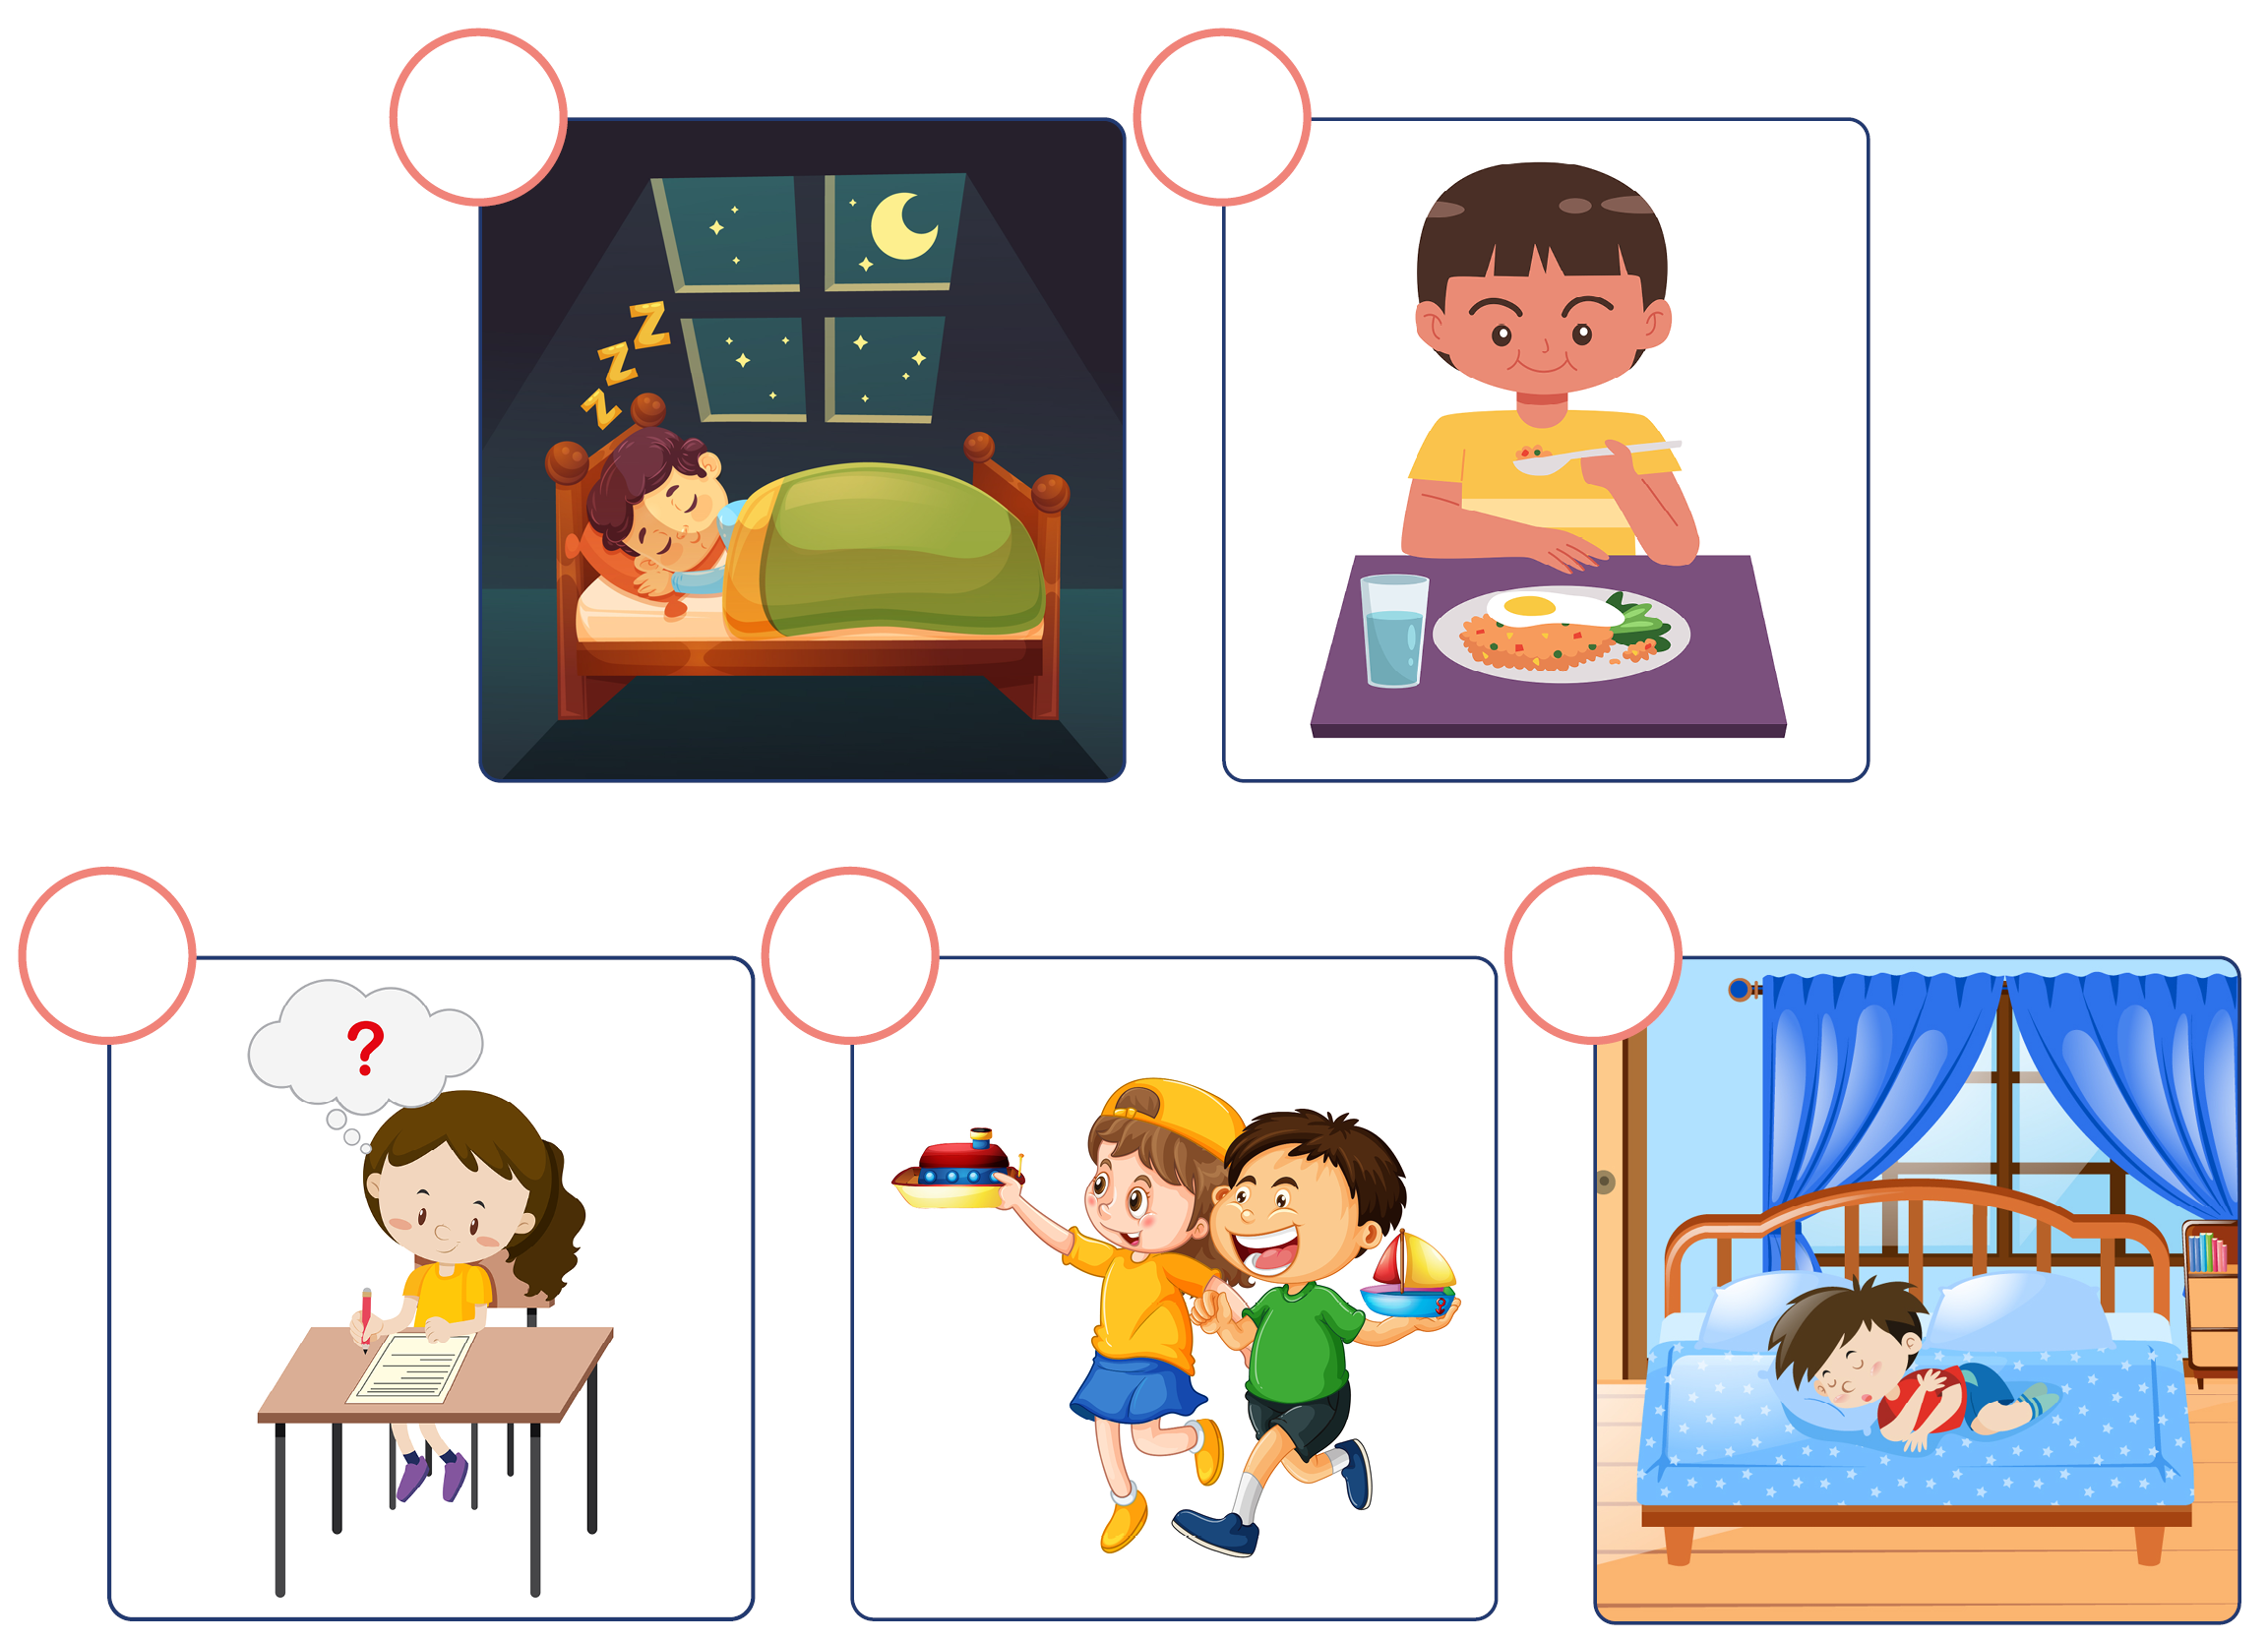
\includegraphics[width=\textwidth]{./media/SAEB_1ANO_MAT_FIGURA52.png}
\end{figure}

\rosa{Da esquerda para a direita, de cima para baixo: 5, 2, 1, 3, 4.}

%\coment{Espera-se que os alunos sigam a ordem dos acontecimentos baseando-se nas próprias rotinas. Aproveite para frisar a importância de se alimentar no horário certo, além de ressaltar a importância de priorizar o momento dos estudos, ou seja, estudar antes de brincar. Esta atividade pode ser utilizada também para os alunos lembrarem a utilização dos números para ordenar. Oriente-os a utilizarem os números de forma ordinal (1º, 2º, 3º etc.).}

\num{5} COMPLETE OS ESPAÇOS EM BRANCO DO CALENDÁRIO A SEGUIR.

\begin{center}
{\large
\begin{tabular}{|ccccccc|}
\hline
\multicolumn{7}{|c|}{\textbf{JANEIRO 2023}} \\ \hline
\multicolumn{1}{|c|}{\textbf{DOM}} & \multicolumn{1}{c|}{\rosa{2ª feira}} & \multicolumn{1}{c|}{\textbf{3ª FEIRA}} & \multicolumn{1}{c|}{\rosa{4ª feira}} & \multicolumn{1}{c|}{\textbf{5ª FEIRA}} & \multicolumn{1}{c|}{\textbf{6ª FEIRA}} & \rosa{Sábado} \\ \hline
\multicolumn{1}{|c|}{1} & \multicolumn{1}{c|}{2} & \multicolumn{1}{c|}{3} & \multicolumn{1}{c|}{\rosa{4}} & \multicolumn{1}{c|}{5} & \multicolumn{1}{c|}{\rosa{6}} & 7 \\ \hline
\multicolumn{1}{|c|}{8} & \multicolumn{1}{c|}{9} & \multicolumn{1}{c|}{\rosa{10}} & \multicolumn{1}{c|}{11} & \multicolumn{1}{c|}{\rosa{12}} & \multicolumn{1}{c|}{13} & 14 \\ \hline
\multicolumn{1}{|c|}{\rosa{15}} & \multicolumn{1}{c|}{16} & \multicolumn{1}{c|}{17} & \multicolumn{1}{c|}{18} & \multicolumn{1}{c|}{19} & \multicolumn{1}{c|}{20} & 21 \\ \hline
\multicolumn{1}{|c|}{22} & \multicolumn{1}{c|}{23} & \multicolumn{1}{c|}{24} & \multicolumn{1}{c|}{\rosa{25}} & \multicolumn{1}{c|}{26} & \multicolumn{1}{c|}{27} & \rosa{28} \\ \hline
\multicolumn{1}{|c|}{29} & \multicolumn{1}{c|}{30} & \multicolumn{1}{c|}{31} & \multicolumn{1}{c|}{} & \multicolumn{1}{c|}{} & \multicolumn{1}{c|}{} &  \\ \hline
\end{tabular}
}
\end{center}

%\coment{Os alunos devem preencher os quadrados faltantes dos dias do mês, assim como dos dias da semana.}

\num{6} BASEANDO-SE NO CALENDÁRIO DA ATIVIDADE ANTERIOR, RESPONDA AO QUE SE PERGUNTA A SEGUIR.

\begin{escolha}[itemsep=-2pt]
\item EM QUE DIA DA SEMANA ESTÁ O DIA 18 DE JANEIRO?

\reduline{Quarta-feira.\hfill}
\linhas{1}

\item QUANTOS SÁBADOS EXISTEM EM JANEIRO DE 2023?

\reduline{São quatro sábados.\hfill}
\linhas{2}

\item EM QUE DIA DA SEMANA COMEÇA ESSE MÊS DE JANEIRO?

\reduline{Domingo.\hfill}
\linhas{1}

\item EM QUE DIA DA SEMANA TERMINA ESSE MÊS DE JANEIRO?

\reduline{Terça-feira.\hfill}
\linhas{1}

\item QUANTOS DOMINGOS EXISTEM NESSE MÊS DE JANEIRO?

\reduline{São cinco domingos.\hfill}
\linhas{2}
\end{escolha}

%\coment{Aproveite para demonstrar que, em alguns meses, pode haver algum dia da semana se repetindo cinco vezes, ou seja, o fato de haver quatro semanas em um mês não significa que haverá sempre quatro repetições de cada dia da semana. Esta atividade é importante para desenvolver no aluno a habilidade de ler o calendário com entendimento.}

\num{7} ANALISE O BLOCO DE NOTAS DE MARCELA. QUANTOS DIAS ELA ESPERARÁ
PELA RESPOSTA DE QUE PRECISA?

%\textless{}Inserir a figura da referência: https://br.freepik.com/vetores-premium/caderno-e-lapis-em-fundo-branco\_10079541.htm\#query=bloco\%20de\%20anota\%C3\%A7\%C3\%B5es\&position=10\&from\_view=search\&track=ais, incluindo o texto conforme o modelo:\textgreater{}

\begin{figure}[H]
\centering
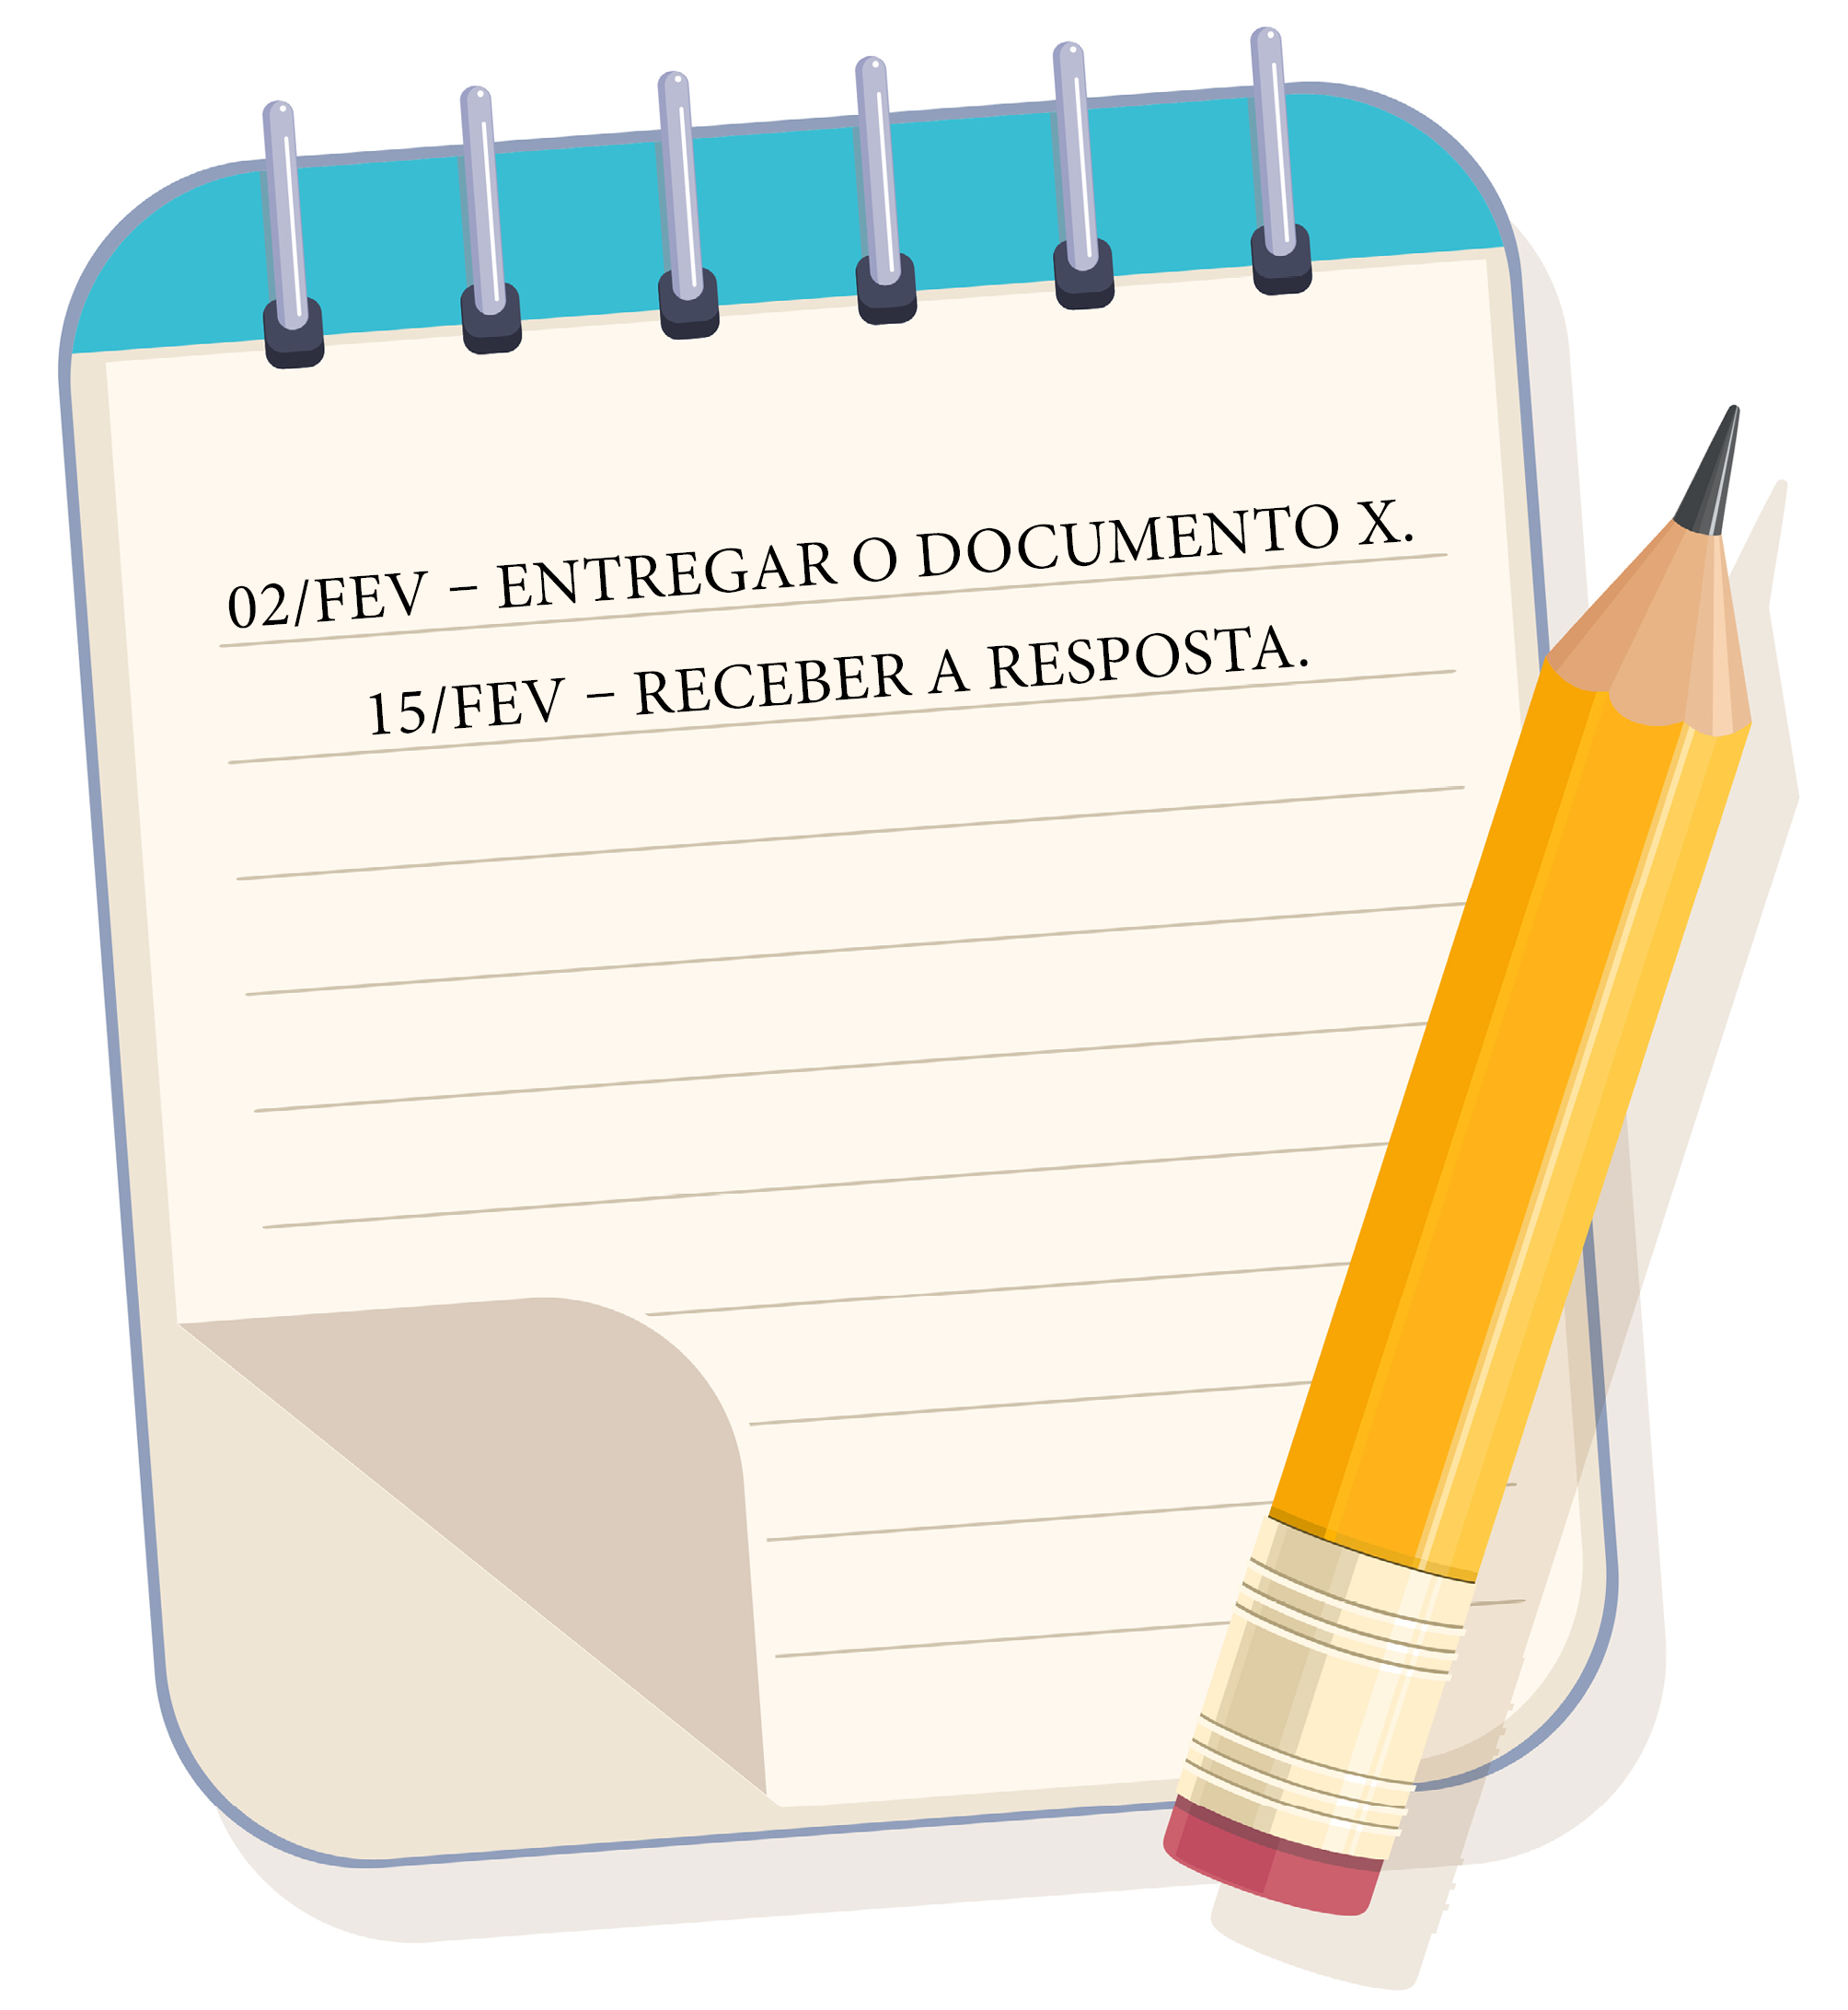
\includegraphics[width=.4\textwidth]{./media/SAEB_1ANO_MAT_FIGURA54.png}
\end{figure}

\reduline{Entre os dias 2 e 15, passam-se 13 dias.\hfill}
\linhas{1}

\num{8} SE O DIA DA SEMANA EM QUE MARCELA ENTREGOU O DOCUMENTO FOSSE
SEXTA-FEIRA, EM QUE DIA DA SEMANA CAIRIA O DIA DA RESPOSTA?

\reduline{Quinta-feira.\hfill}
\linhas{1}

\num{9} UMA COMPETIÇÃO DE FUTEBOL DE SALÃO DUROU 7 DIAS.
SE A COMPETIÇÃO COMEÇOU NO DIA 10 DE OUTUBRO DE 2021, SÁBADO, EM QUE
DATA TERMINOU O CAMPEONATO?

\begin{escolha}[itemsep=-2pt]
\item \textbf{ANO:} \reduline{2021.\hfill}

\item \textbf{MÊS:} \reduline{Outubro.\hfill}

\item \textbf{DIA DO MÊS:} \reduline{16.\hfill}

\item \textbf{DIA DA SEMANA:} \reduline{Sexta-feira.\hfill}
\end{escolha}

\num{10} ANALISE OS RELÓGIOS DIGITAIS DA IMAGEM. DEPOIS, RESPONDA AO QUE SE PERGUNTA A SEGUIR.

%\textless{}Inserir a figura da referência: https://br.freepik.com/vetores-premium/um-conjunto-de-relogios-digitais-numeros-eletronicos-ilustracao-vetorial\_32708528.htm\#query=rel\%C3\%B3gio\%20digital\&position=16\&from\_view=search\&track=ais, inserindo as identificações dos relógios, conforme o modelo a seguir.\textgreater{}

\begin{figure}[htpb!]
\centering
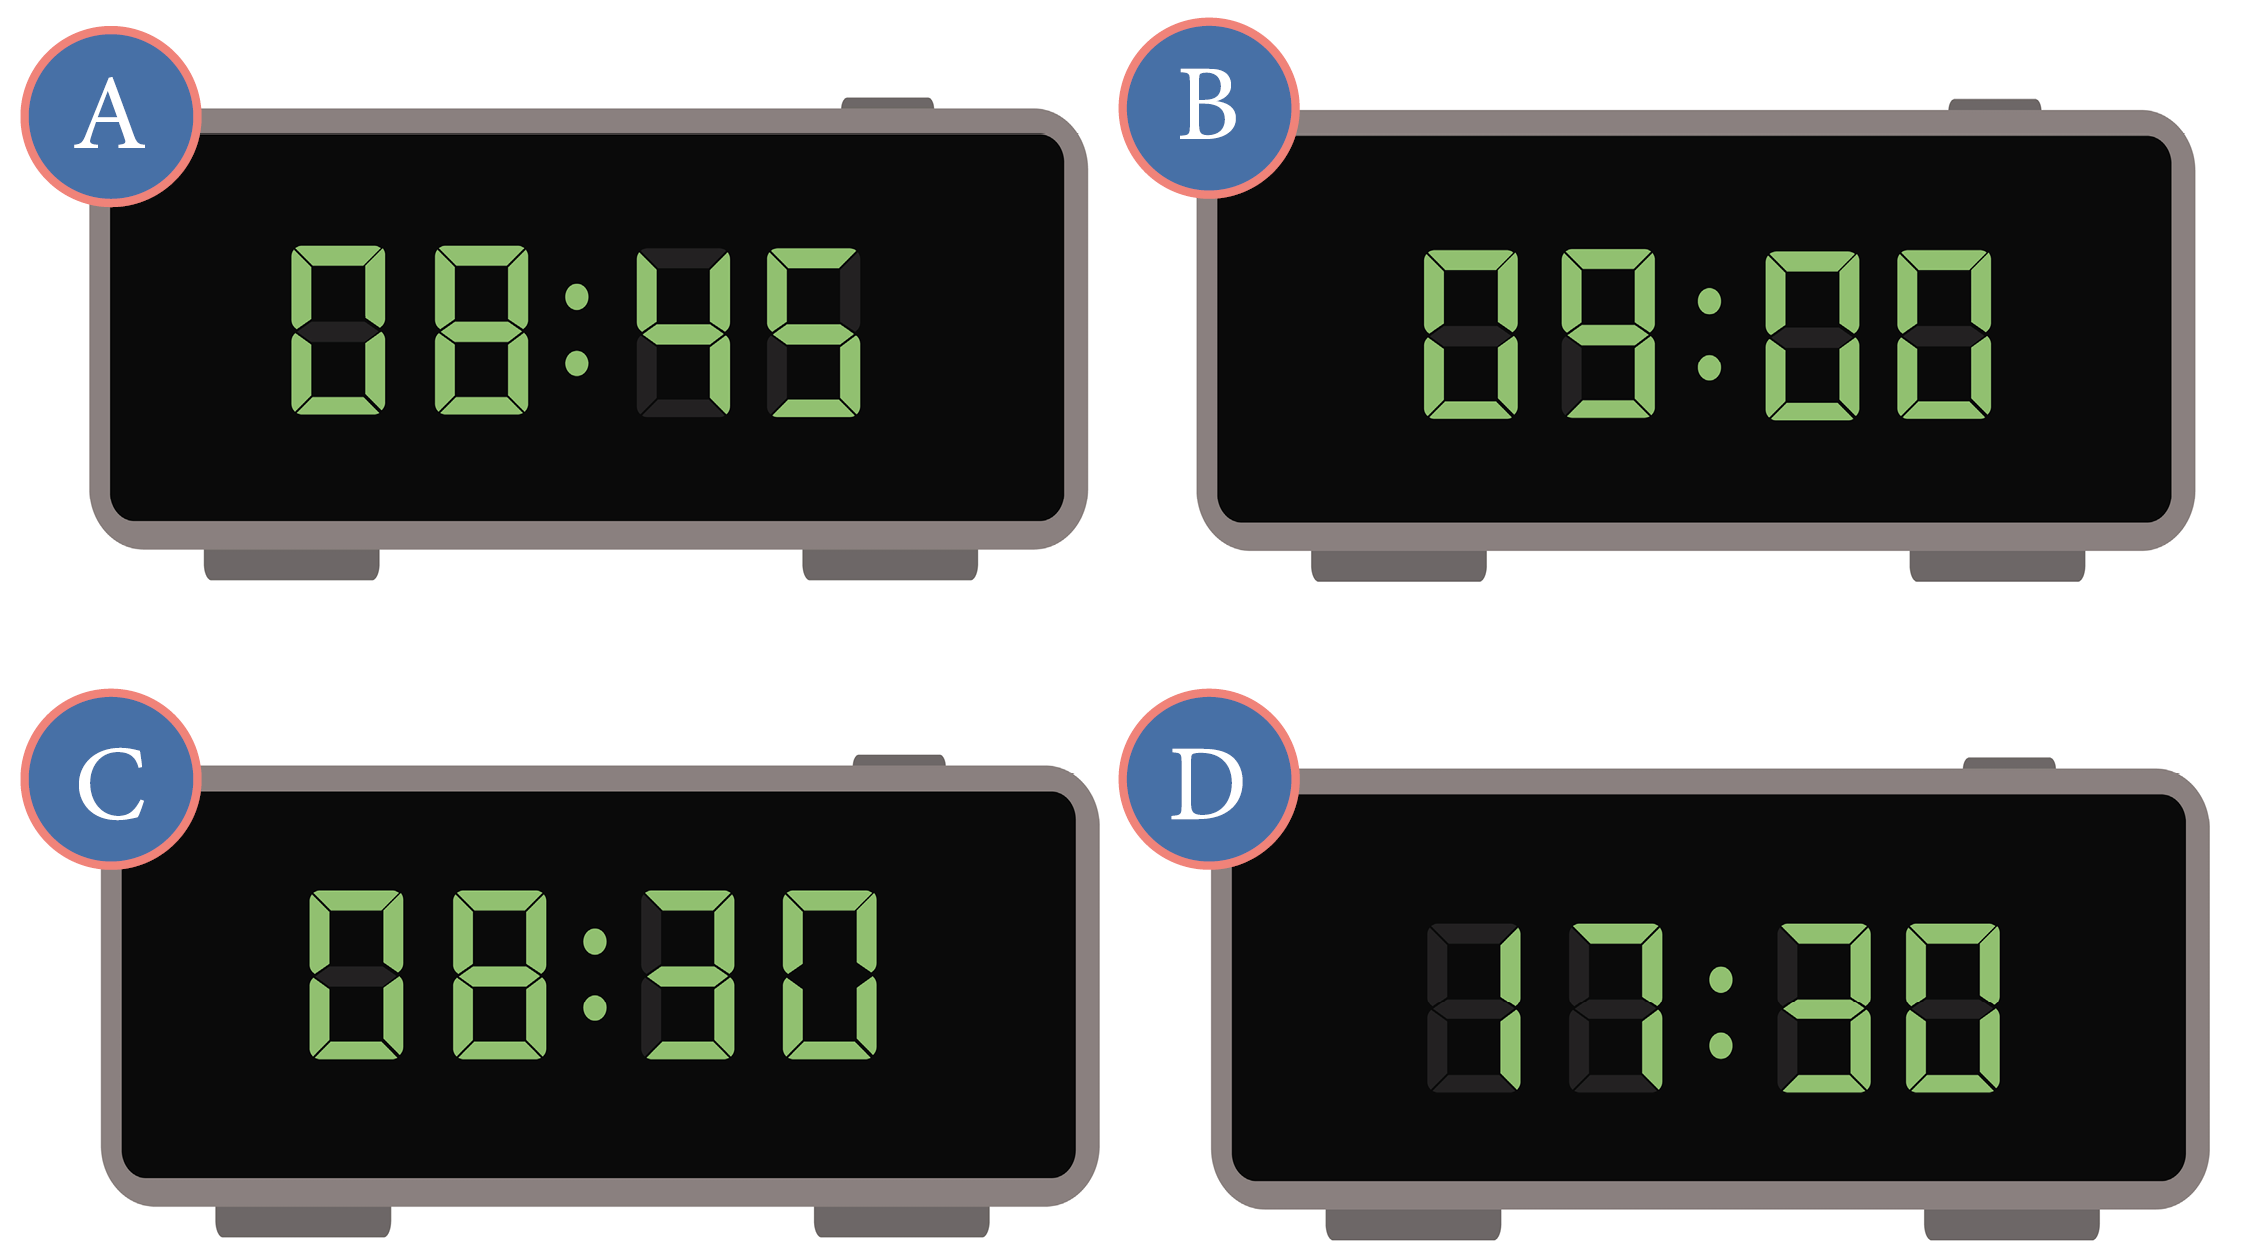
\includegraphics[width=\textwidth]{./media/SAEB_1ANO_MAT_FIGURA56.png}
\end{figure}

\begin{escolha}
\item QUAL É A DIFERENÇA ENTRE O HORÁRIO DO RELÓGIO \textbf{A} E O DO RELÓGIO \textbf{B}?

\reduline{Uma hora e quarenta e cinco minutos. 01:45:00.\hfill}

\item QUAL É A DIFERENÇA ENTRE O HORÁRIO DO RELÓGIO \textbf{C} E O DO RELÓGIO \textbf{A}?

\reduline{Quinze minutos. 00:15:00.\hfill}

\item QUAL É A DIFERENÇA ENTRE O HORÁRIO DO RELÓGIO \textbf{B} E O DO RELÓGIO \textbf{D}?

\reduline{Oito horas e trinta minutos. 08:30:00.\hfill}

\item QUAL É A DIFERENÇA ENTRE O HORÁRIO DO RELÓGIO \textbf{C} E O DO RELÓGIO \textbf{D}?

\reduline{Nove horas. 09:00:00.\hfill}
\end{escolha}

%\coment{Oriente os alunos a darem respostas neste formato: hh:mm:ss.}

% \num{11} PARA ACORDAR, MARIANO AJUSTOU O ALARME DO CELULAR PARA O HORÁRIO MOSTRADO A SEGUIR.\bigskip

% %\textless{}https://br.freepik.com/vetores-gratis/smartphone-de-tela-de-alarme\_2921841.htm\#query=relogio\%20celular\&position=48\&from\_view=search\&track=ais.\textgreater{}

% \begin{minipage}{.4\textwidth}
% 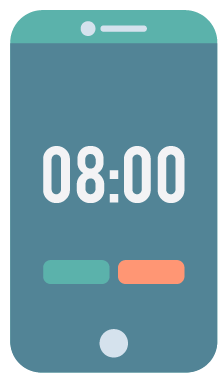
\includegraphics[width=.3\textwidth]{./media/SAEB_1ANO_MAT_FIGURA57.png}
% \end{minipage}
% \begin{minipage}{.6\textwidth}
% ELE LEVANTOU-SE, ARRUMOU-SE, TOMOU CAFÉ DA MANHÃ E FOI PARA O TRABALHO. CHEGOU AO TRABALHO 1 HORA E 35 MINUTOS DEPOIS DE ACORDAR. A QUE HORAS ELE CHEGOU AO TRABALHO?
% \end{minipage}\bigskip\bigskip

% \reduline{09:35:00.\hfill}

% \pagebreak
% \num{12} PEDRO ACORDOU ÀS 07:30 DA MANHÃ.

% %https://br.freepik.com/vetores-gratis/um-menino-dormindo-profundamente\_23807622.htm\#query=PEDRINHO\%20ACORDANDO\&position=5\&from\_view=search\&track=ais.\textgreater{}; https://br.freepik.com/vetores-gratis/menino-de-pijama-segurando-a-escova-de-dentes-e-pasta-de-dente\_27547013.htm\#query=ESCOVAR\%20OS\%20DENTES\&position=32\&from\_view=search\&track=ais https://br.freepik.com/vetores-gratis/um-menino-feliz-comendo-na-mesa\_18973385.htm\#query=CAF\%C3\%81\%20DA\%20MANH\%C3\%83\%20MENINO\&position=12\&from\_view=search\&track=ais; https://br.freepik.com/vetores-premium/um-menino-brincando-com-gato-fofo\_29183474.htm\#page=2\&query=BRINCANDO\%20COM\%20O\%20GATO\&position=6\&from\_view=search\&track=ais. \textgreater{} \begin{quote} 

% \begin{figure}[htpb!]
% \centering
% 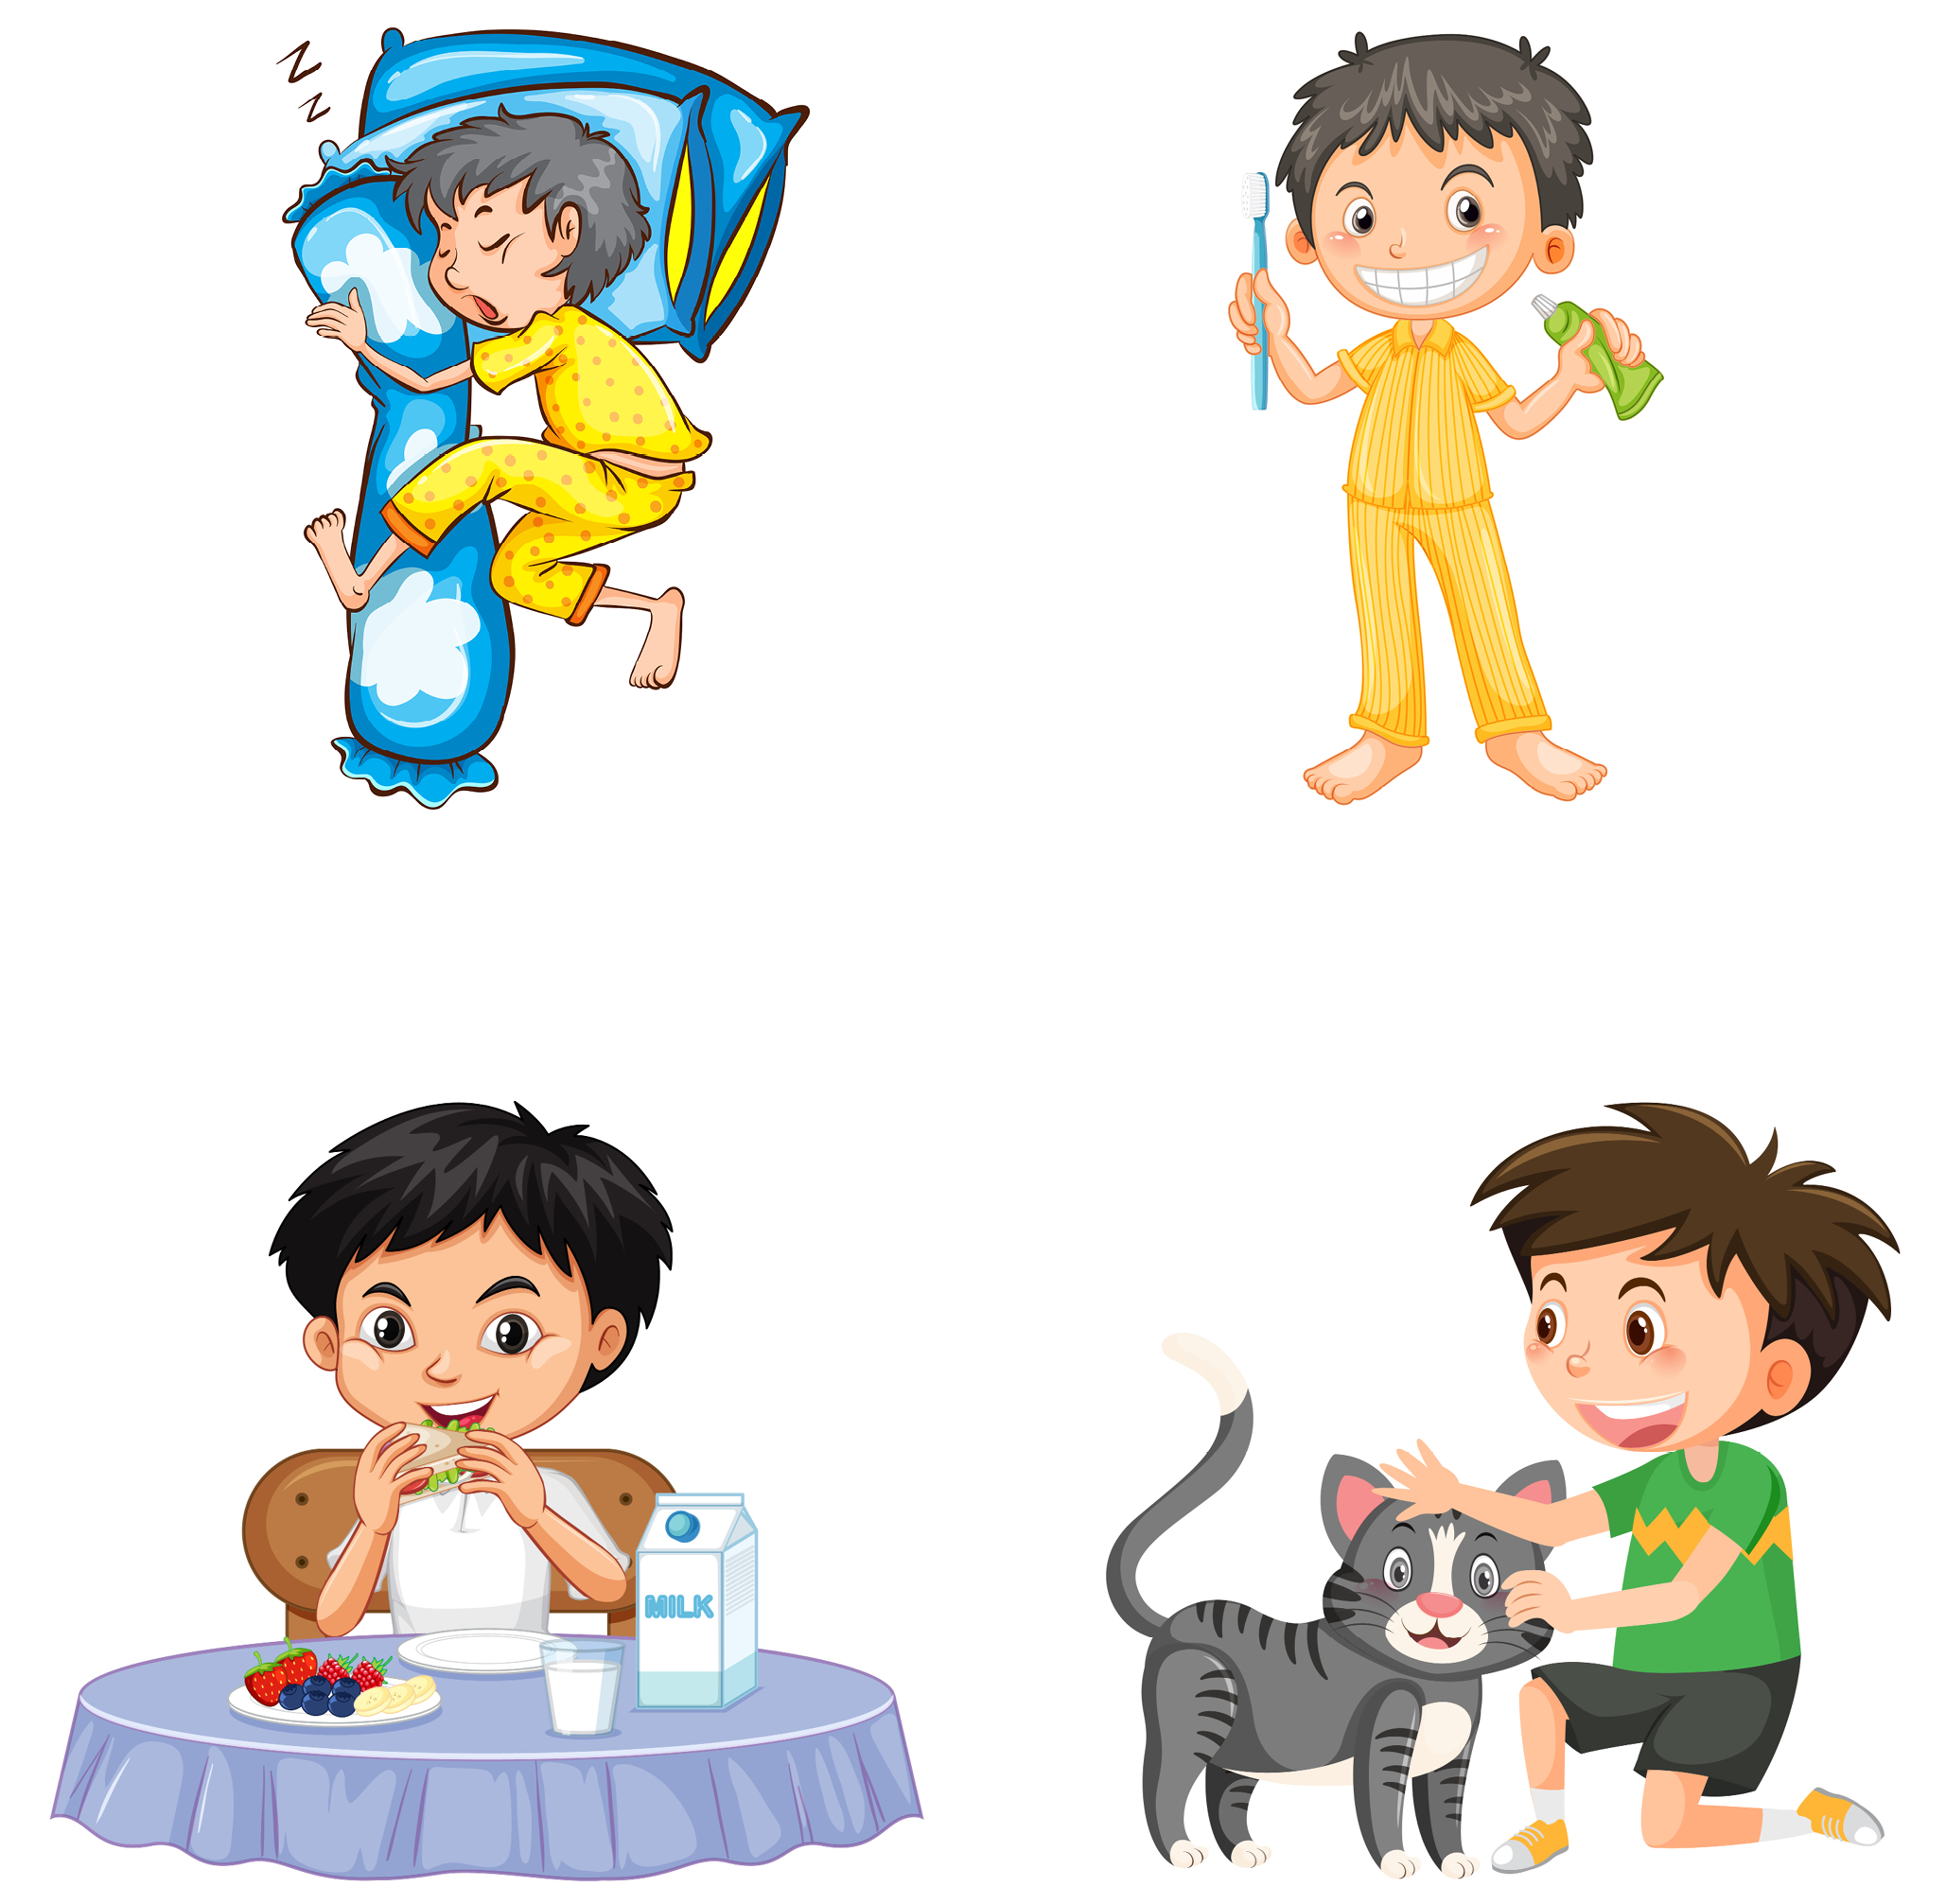
\includegraphics[width=.6\textwidth]{./media/SAEB_1ANO_MAT_FIGURA58.png}
% \end{figure}

% DEPOIS, DEMOROU 15 MINUTOS PARA IR AO BANHEIRO E ESCOVAR OS DENTES.
% DEMOROU MAIS 20 MINUTOS PARA TOMAR O CAFÉ DA MANHÃ. ANTES DE SAIR,
% AINDA FICOU 5 MINUTOS BRINCANDO COM O GATO. ENTÃO SAIU PARA A ESCOLA.

% PINTE NO RELÓGIO A SEGUIR O HORÁRIO EM QUE PEDRO SAIU PARA IR À ESCOLA.

% %\textless{}Inserir uma figura de um relógio, com os números em branco para o aluno preencher, conforme o modelo a seguir:\textgreater{}

% \begin{figure}[htpb!]
% \centering
% 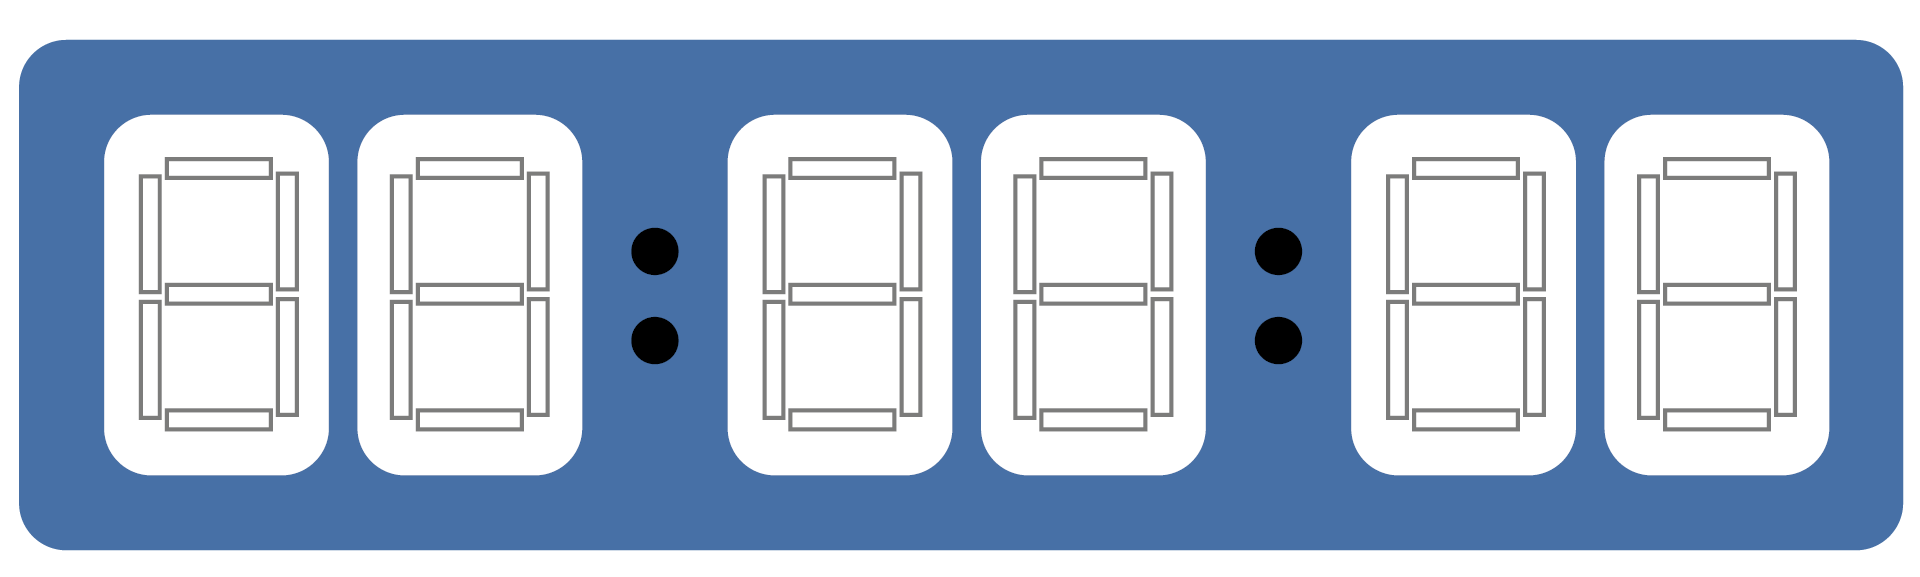
\includegraphics[width=\textwidth]{./media/SAEB_1ANO_MAT_FIGURA59.png}
% \end{figure}

% %Oriente os alunos a pintarem os quadradinhos para formar o horário, da mesma forma como aparecem nos relógios digitais.
% \coment{A pintura deve formar o horário 08:10:00}

\section*{TREINO}

\num{1} ANALISE O CALENDÁRIO A SEGUIR.

% \begin{figure}[H]
% \centering
% 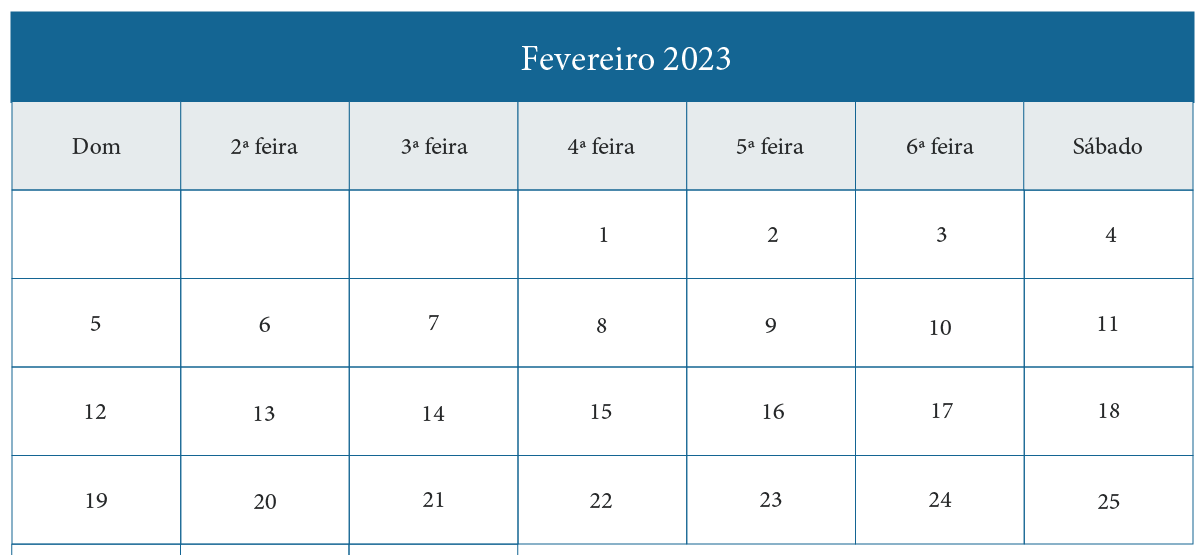
\includegraphics[width=\textwidth]{./media/SAEB_1ANO_MAT_FIGURA61.png}
% \end{figure}


\begin{table}[!ht]
    \centering
    \begin{tabular}{|l|l|l|l|l|l|l|}
    \hline
        \textbf{DOM} & \textbf{SEG} & \textbf{TER} & \textbf{QUA} & \textbf{QUI} & \textbf{SEX} & \textbf{SÁB} \\ \hline
        ~ & ~ & ~ & 1 & 2 & 3 & 4 \\ \hline
        5 & 6 & 7 & 8 & 9 & 10 & 11 \\ \hline
        12 & 13 & 14 & 15 & 16 & 17 & 18 \\ \hline
        19 & 20 & 21 & 22 & 23 & 24 & 25 \\ \hline
        26 & 27 & ~ & ~ & ~ & ~ & ~ \\ \hline
    \end{tabular}
\end{table}

A ÚLTIMA SEGUNDA-FEIRA DESSE MÊS SERÁ O DIA

\begin{escolha}
\item 6.

\item 26.

\item 27.

\item 28.
\end{escolha}

\num{2} ANALISE AS FIGURAS.

%\textless{}https://br.freepik.com/vetores-gratis/antecedentes-da-paisagem-plana-em-tons-roxos\_1001699.htm\#query=anoitecer\&position=2\&from\_view=search\&track=sph; https://br.freepik.com/vetores-gratis/paisagem-do-por-do-sol-com-lago-nuvens-no-ceu-vermelho-silhuetas-nas-colinas-e-arvores-na-costa\_12407808.htm\#query=amanhecer\&position=1\&from\_view=search\&track=sph

%; https://br.freepik.com/vetores-gratis/paisagem-de-primavera-desenhados-a-mao\_6804642.htm\#query=meio\%20dia\%20paisagem\&position=13\&from\_view=search\&track=ais

%; https://br.freepik.com/vetores-gratis/lua-cheia-noite-oceano-cartoon-ilustracao\_6690817.htm\#query=noite\%20paisagem\&position=10\&from\_view=search\&track=ais

\begin{figure}[H]
\centering
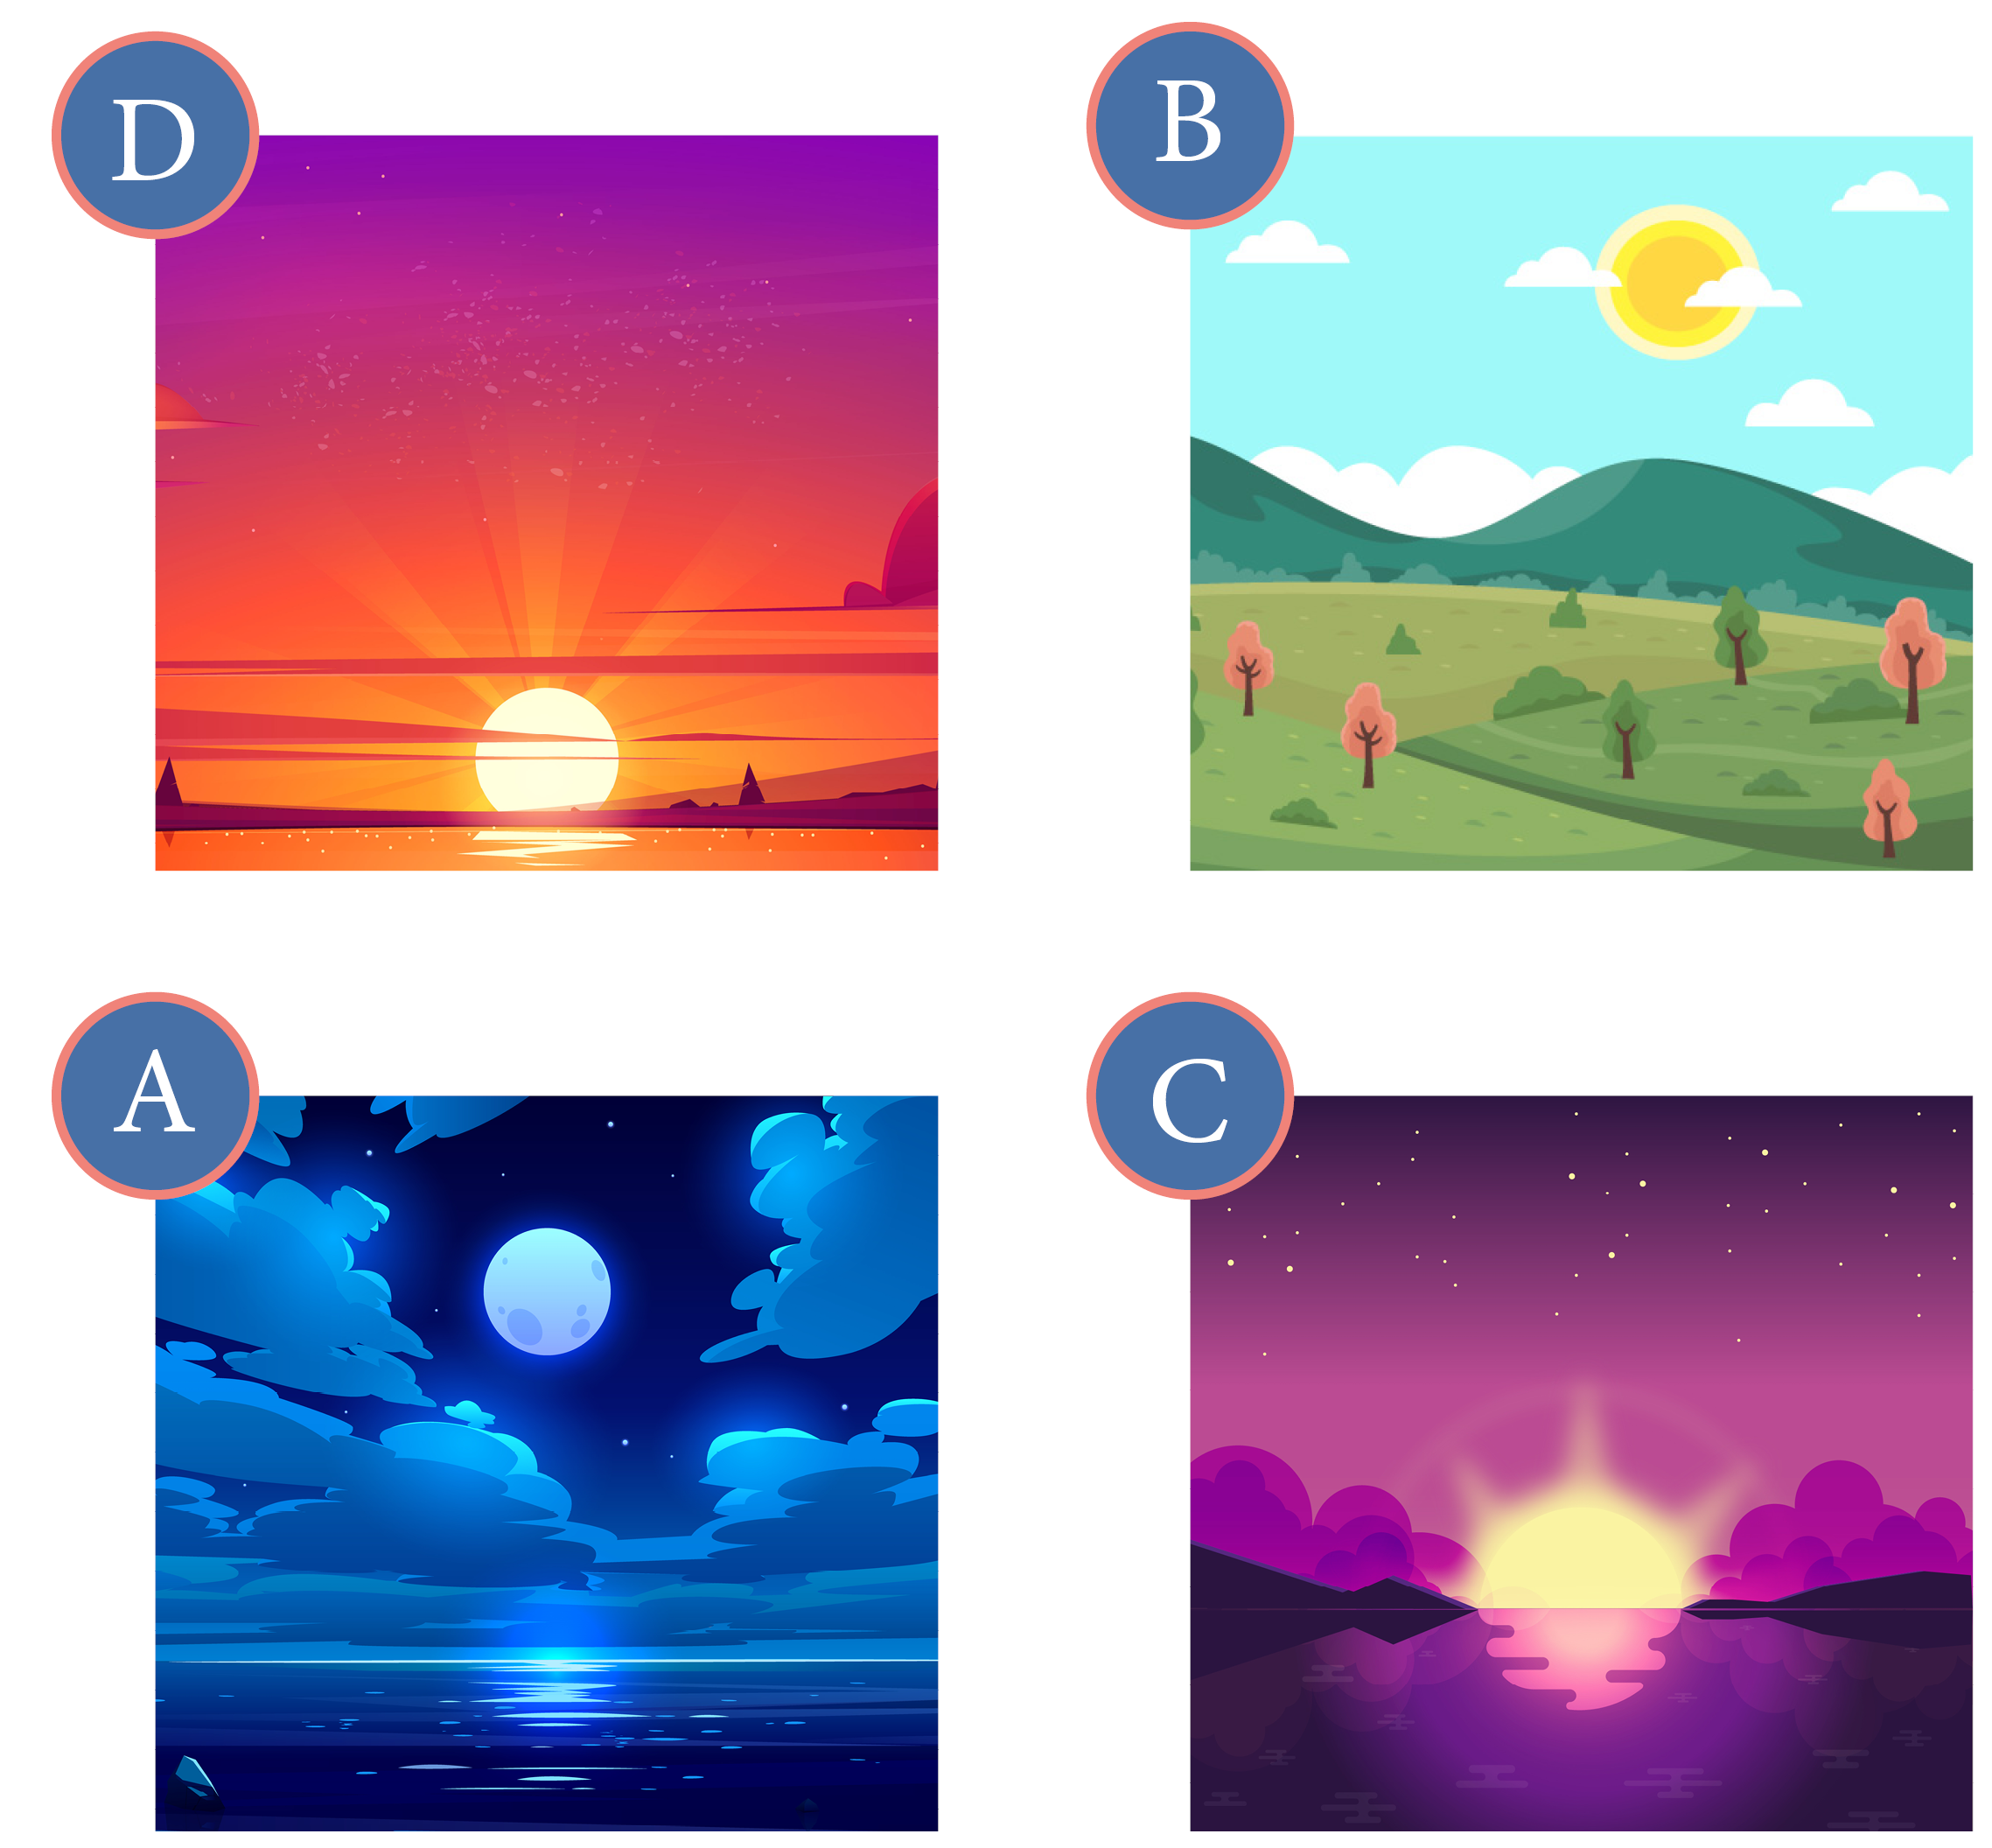
\includegraphics[width=.6\textwidth]{./media/SAEB_1ANO_MAT_FIGURA62.png}
\end{figure}

INDIQUE QUAL É A SEQUÊNCIA CORRETA DE ACONTECIMENTOS.

\begin{escolha}
\item A, B, C, D.

\item B, A, C, D.

\item C, B, A, D.

\item D, B, C, A.
\end{escolha}

\num{3} O BALÃO REPRESENTADO NA FOTOGRAFIA A SEGUIR LEVANTOU 
VOO ÀS 06:45 E VOLTOU AO CHÃO ÀS 07:45.

\begin{figure}[H]
\centering
\includegraphics[width=.9\textwidth]{./media/image114.jpg}
\end{figure}

QUAL FOI A DURAÇÃO DO VOO?

\begin{escolha}
\item 15 MINUTOS.

\item 45 MINUTOS.

\item 1 HORA.

\item 1 HORA E 45 MINUTOS.
\end{escolha}

\begin{comment}

\chapter{MESADA}
\markboth{Módulo 5}{}

%\coment{Neste módulo, vamos desenvolver nos alunos a habilidade de reconhecerem o valor das cédulas de dinheiro, assim como das moedas, por meio da identificação de suas cores e dos próprios números que as representam. Também vamos desenvolver nos alunos a capacidade de resolverem situações-problema que favorecem o trabalho com o tema contemporâneo transversal educação financeira.} 
\vspace*{-2cm}

\section{HABILIDADES DO SAEB:}

\begin{itemize}
\item Relacionar valores de moedas e/ou cédulas do sistema monetário
brasileiro, com base nas imagens desses objetos.

\item Resolver problemas que envolvam moedas e/ou cédulas do sistema
monetário brasileiro.
\end{itemize}

\subsection{Habilidade da BNCC}

\begin{itemize}
\item EF01MA19.
\end{itemize}

\conteudo{
OBSERVE ESTA TABELA, QUE
MOSTRA AS CÉDULAS DO DINHEIRO QUE USAMOS NO BRASIL. O NOME DO NOSSO
DINHEIRO É \textbf{REAL} E O SÍMBOLO QUE O REPRESENTA É ESTE: \textbf{R\$}.

\centering{\includegraphics[width=.7\textwidth]{./media/SAEB_1ANO_MAT_FIGURA63.png}}
}

\conteudo{
AGORA, OBSERVE AS MOEDAS E PERCEBA SUAS DIFERENÇAS. A MOEDA DE MENOR VALOR É A DE 1 CENTAVO, QUE REPRESENTA UM REAL DIVIDIDO EM 100 PARTES. A MOEDA DE MAIOR VALOR É A DE 1 REAL, QUE EQUIVALE A CEM CENTAVOS.

\includegraphics[width=\textwidth]{./media/SAEB_1ANO_MAT_FIGURA64.png}
}

%\coment{É importante que as crianças usem as peculiaridades de cada cédula, como a cor predominante e o animal estampado, para identificar o valor, além do número impresso. Se possível, mostre aos alunos cédulas verdadeiras, com o intuito de lhes mostrar a marca d'água e outras características que apontem para sua autenticidade.}


%\textless{}https://br.freepik.com/fotos-gratis/dinheiro-moedas-brasileiras-escada\_23076933.htm\#page=9\&query=REAIS\%20moedas\&position=39\&from\_view=search\&track=ais\textgreater{}

\section{ATIVIDADES}

\num{1} MARQUE, NA ETIQUETA, O VALOR DE CADA PRODUTO.

%\textless{}https://br.freepik.com/vetores-gratis/colecao-de-brinquedos-de-natal-desenhada-a-mao\_11105919.htm\#query=brinquedos\%20com\%20etiquetas\&position=14\&from\_view=search\&track=ais. Inserir na coluna da direita uma figura de etiqueta para o aluno preencher o valor da mercadoria.\textgreater{}

\begin{figure}[htpb!]
\includegraphics[width=\textwidth]{./media/SAEB_1ANO_MAT_FIGURA65.png}
\end{figure}

\pagebreak

\begin{figure}[htpb!]
\includegraphics[width=\textwidth]{./media/SAEB_1ANO_MAT_FIGURA66.png}
\end{figure}

\begin{figure}[htpb!]
\includegraphics[width=\textwidth]{./media/SAEB_1ANO_MAT_FIGURA67.png}
\end{figure}

\begin{figure}[htpb!]
\includegraphics[width=\textwidth]{./media/SAEB_1ANO_MAT_FIGURA68.png}
\end{figure}

\pagebreak

\num{2} ESCREVA POR EXTENSO OS VALORES EM REAIS.

%\textless{}Inserir a tabela conforme o modelo abaixo\textgreater{}

\begin{escolha}
\item R\$ 135,60 \reduline{Cento e trinta e cinco reais e sessenta centavos.\hfill}

\item R\$ 465,00 \reduline{Quatrocentos e sessenta e cinco reais.\hfill}

\item R\$ 59,30 \reduline{Cinquenta e nove reais e trinta centavos.\hfill}

\item R\$ 74,15 \reduline{Setenta e quatro reais e quinze centavos.\hfill}

\item R\$ 63,20 \reduline{Sessenta e três reais e vinte centavos.\hfill}

\item R\$ 15,15 \reduline{Quinze reais e quinze centavos.\hfill}
\end{escolha}

\num{3} LIGUE CORRETAMENTE CADA VALOR A UMA IMAGEM.

%\textless{}https://br.freepik.com/fotos-gratis/dinheiro-moedas-brasileiras-1-real\_22809605.htm\#query=moeda\%20de\%201\%20real\%20dineiro\%20barssileiro\&position=1\&from\_view=search\&track=ais; https://br.freepik.com/fotos-gratis/dinheiro-moedas-brasileiras-5-centavos\_22781620.htm\#query=moeda\%20de\%205\%20centavos\%20dineiro\%20barssileiro\&position=2\&from\_view=search\&track=ais; https://br.freepik.com/fotos-gratis/dinheiro-moedas-brasileiras-10-centavos\_22781622.htm\#query=moeda\%20de\%2010\%20centavos\%20dineiro\%20barssileiro\&position=6\&from\_view=search\&track=ais;

\begin{minipage}{.7\textwidth}
\includegraphics[width=\textwidth]{./media/SAEB_1ANO_MAT_FIGURA70.png}
\end{minipage}
\begin{minipage}{.3\textwidth}
\coment{Se os alunos tiverem alguma dificuldade com esta atividade,
uma vez que ainda não tiveram contato com números fracionários, ajude-os
a associarem os valores às imagens das moedas.}
\end{minipage}

\pagebreak
\num{4} PREENCHA CADA ESPAÇO COM A QUANTIDADE DE CÉDULAS NECESSÁRIAS PARA COMPRAR O ITEM CORRESPONDENTE. USE SOMENTE CÉDULAS.

%\textless{}https://www.istockphoto.com/br/foto/notas-de-dinheiro-do-brasil-em-composto-detalhes-de-notas-de-200-50-10-5-e-2-reais-gm1280319451-378658163?phrase=200\%20REAIS. Inserir quadros para que os alunos consigam colocar a quantidade de notas necessárias.\textgreater{}

\begin{escolha}
\item UM CARRINHO DE R\$ 100,00.

\includegraphics[width=.8\textwidth]{./media/SAEB_1ANO_MAT_FIGURA71.png}

\item UMA BONECA DE R\$ 70,00.

\includegraphics[width=.8\textwidth]{./media/SAEB_1ANO_MAT_FIGURA72.png}

\item UMA CALÇA DE R\$ 137,00.

\includegraphics[width=.8\textwidth]{./media/SAEB_1ANO_MAT_FIGURA73.png}

\item UMA SAIA DE R\$ 85,00.

\includegraphics[width=.8\textwidth]{./media/SAEB_1ANO_MAT_FIGURA74.png}

\item UM CHOCOLATE DE R\$ 6,00.

\includegraphics[width=.8\textwidth]{./media/SAEB_1ANO_MAT_FIGURA75.png}

\item UM PAR DE ÓCULOS ESCUROS DE R\$ 450,00.

\includegraphics[width=.8\textwidth]{./media/SAEB_1ANO_MAT_FIGURA76.png}
\end{escolha}

%\coment{Exceto para o chocolate, de R\$ 6,00, há mais de uma combinação possível para cada item. É de suma importância trabalhar com os alunos as respostas diferentes.}

\pagebreak
\num{5} PREENCHA CADA CÍRCULO COM A QUANTIDADE DE MOEDAS NECESSÁRIAS PARA COMPRAR O ITEM CORRESPONDENTE. USE SOMENTE MOEDAS.

%\textless{}https://br.freepik.com/fotos-gratis/dinheiro-moedas-brasileiras-escada\_23076933.htm\#page=9\&query=REAIS\%20moedas\&position=39\&from\_view=search\&track=ais. Inserir os círculos abaixo de cada moeda para o aluno preencher a quantidade necessária.\textgreater{}

\begin{escolha}
\item UM PIRULITO DE R\$ 0,35 (TRINTA E CINCO CENTAVOS).

\includegraphics[width=.7\textwidth]{./media/SAEB_1ANO_MAT_FIGURA77.png}

\item UMA BALA DE R\$ 0,15 (QUINZE CENTAVOS).

\includegraphics[width=.7\textwidth]{./media/SAEB_1ANO_MAT_FIGURA78.png}

\item UM APITO DE R\$ 0,30 (TRINTA CENTAVOS).

\includegraphics[width=.7\textwidth]{./media/SAEB_1ANO_MAT_FIGURA79.png}

\item UM CHAVEIRO DE SUPER-HERÓI DE R\$ 3,75 (TRÊS REAIS E SETENTA E CINCO

\includegraphics[width=.7\textwidth]{./media/SAEB_1ANO_MAT_FIGURA80.png}
\end{escolha}

%\coment{Os alunos precisarão de uma ajuda extra por não conhecerem números fracionários.}

\pagebreak

\num{6} JOÃO E BIANCA GANHARAM R\$ 10,00 (CADA UM). JOÃO COMPROU UM DOCE DE R\$ 6,00,
E BIANCA COMPROU UM DOCE DE R\$ 5,00. SOBRE ESSA SITUAÇÃO, RESPONDA AO QUE SE PERGUNTA A SEGUIR.

\begin{escolha}
\item QUANTO JOÃO E BIANCA GANHARAM JUNTOS? RESPONDA COM ALGARISMOS E POR EXTENSO.
\reduline{R\$ 10,00 + R\$ 10,00 = R\$ 20,00 -- vinte reais.\hfill}

\item QUANTO JOÃO E BIANCA GASTARAM JUNTOS?
\reduline{R\$ 6,00 + R\$ 5,00 = R\$ 11,00 -- onze reais.\hfill}

\item QUANTO DINHEIRO SOBROU PARA JOÃO E BIANCA JUNTOS?
\reduline{R\$ 20,00 -- R\$ 11,00 = R\$ 9,00 -- nove reais.\hfill}

\item DESENHE, INCLUSIVE COM CORES, AS CÉDULAS E AS MOEDAS DO REAL. TENTE SE LEMBRAR DO MAIOR NÚMERO POSSÍVEL DE DETALHES DE CADA UMA.
\end{escolha}

\begin{mdframed}[linewidth=2pt,linecolor=salmao,roundcorner=10pt]
\vspace{7cm}
\end{mdframed}

\pagebreak
\section{TREINO}

\num{1} OBSERVE A IMAGEM A SEGUIR.

%\textless{}https://www.istockphoto.com/br/foto/brasileiro-dinheiro-novo-gm492494099-40521892?phrase=10\%20REAIS\textgreater{}

\begin{figure}[htpb!]
\centering
\includegraphics[width=\textwidth]{./media/SAEB_1ANO_MAT_FIGURA82.jpg}
\end{figure}

O VALOR DA CÉDULA REPRESENTADA NA IMAGEM É DE


\begin{escolha}
\item R\$ 0,10.

\item R\$ 1,00.

\item R\$ 10,00.

\item R\$ 100,00.
\end{escolha}

\pagebreak
\num{2} CRISTIANO COMPROU UM CHAPÉU DE R\$ 75,00. DE QUE FORMA ELE PODE TER PAGADO POR ESSE CHAPÉU?

\begin{escolha}
\item COM DUAS CÉDULAS DE R\$ 50,00.

\item COM TRÊS CÉDULAS DE R\$ 25,00.

\item COM TRÊS CÉDULAS DE R\$ 10,00.

\item COM TRÊS CÉDULAS DE R\$ 5,00.
\end{escolha}


\num{3} ANA PRECISA PAGAR UMA FATURA DE R\$ 182,00. ELA ESTÁ COM UMA CÉDULA DE R\$ 100,00, UMA CÉDULA DE R\$ 50,00, UMA CÉDULA DE R\$ 20,00 E DUAS CÉDULAS DE R\$ 5,00. PODE-SE AFIRMAR QUE ANA

\begin{escolha}
\item TEM O VALOR EXATO PARA PAGAR A FATURA.

\item CONSEGUE COMPLETAR O VALOR COM UMA MOEDA SÓ.

\item PRECISA TER PELO MENOS MAIS UMA CÉDULA DE R\$ 2,00.

\item CONTINUARIA SEM O VALOR CERTO MESMO COM MAIS UMA CÉDULA DE R\$ 5,00.
\end{escolha}

\chapter{SERÁ QUE VAI CHOVER?}
\markboth{Módulo 6}{}

%\coment{Neste módulo, vamos trabalhar a habilidade dos alunos de perceber que alguns fatos podem ser previsíveis, e outros não. A noção de probabilidade matemática pode ser um pouco complexa para crianças da idade, porém, com situações do cotidiano, pode-se fazer com que elas percebam que é mais provável que isto ou aquilo aconteça.}

\section{HABILIDADE DO SAEB}

\begin{itemize}
\item Classificar resultados de eventos cotidianos aleatórios como ``pouco
prováveis'', ``muito prováveis'', ``certos'' ou ``impossíveis''.
\end{itemize}

\subsection{Habilidade da BNCC}

\begin{itemize}
\item EF01MA20.
\end{itemize}


\conteudo{
COMO É POSSIVEL SABER SE VAI CHOVER OU NÃO? EXISTE TODA UMA CIÊNCIA POR TRÁS DESSA PREVISÃO: A METEOROLOGIA.
NO ENTANTO, SE OLHAMOS PARA O CÉU E O VEMOS ESCURO, CRIAMOS A EXPECTATIVA DE VAI CHOVER, MESMO SEM USAR UMA CIÊNCIA MAIS PRECISA. NA METEOROLOGIA, UMA SÉRIE DE ACONTECIMENTOS
PERMITE AOS TÉCNICOS FAZER UMA PREVISÃO DO TEMPO, MAS NÓS TAMBÉM PODEMOS FAZER PREVISÕES NO DIA A DIA. PODEMOS DIZER QUE EXISTEM QUATRO POSSIBILIDADES. POR EXEMPLO:

%\textless{}Inserir um quadro conforme o modelo a seguir, utilizando as referências: https://br.freepik.com/vetores-premium/pequeno-elefante-voar-para-o-ceu\_6579577.htm\#query=elefante\%20voando\&position=9\&from\_view=search\&track=ais; https://br.freepik.com/vetores-gratis/fundo-plano-do-polo-norte-da-temporada-de-inverno\_33138109.htm\#query=neve\&position=11\&from\_view=search\&track=sph (alterar a placa colocando nela Brasil no lugar de polo norte.; https://br.freepik.com/vetores-gratis/ilustracao-de-calor-de-verao-plana-com-homem-na-cadeira\_27995494.htm\#query=ver\%C3\%A3o\%20calor\&position=0\&from\_view=search\&track=ais; https://br.freepik.com/vetores-premium/jogador-de-futebol-jogando-futebol-em-pe\_33803714.htm\#query=bola\%20jogada\%20pra\%20cima\&position=7\&from\_view=search\&track=ais.\textgreater{}

\centering{\includegraphics[width=.7\textwidth]{./media/SAEB_1ANO_MAT_FIGURA83.png}}
}

%\coment{É importante ressaltar com os alunos que, no Brasil, é raro nevar, mas pode acontecer, principalmente na região Sul. Vale ressaltar também que nem todos os dias do verão são quentes, ou seja, a temperatura pode cair em alguns dias.}

\section{ATIVIDADES}

\num{1} PINTE OS CÍRCULOS COM AS SITUAÇÕES IMPOSSÍVEIS NO QUADRO A SEGUIR. PINTE
DA COR QUE VOCÊ PREFERIR.

%\textless{}criar um quadro com as situações descritas conforme o modelo a seguir.\textgreater{} 

\begin{figure}[htpb!]
\centering
\includegraphics[width=.8\textwidth]{./media/SAEB_1ANO_MAT_FIGURA84.png}
\end{figure}

%\coment{Esta atividade pode ser importante para trabalhar a habilidade de leitura dos alunos. As situações impossíveis são: céu ficando verde, tesoura falando, jacaré voando, leão miando, unicórnios existindo, chuva caindo para cima e árvore andando.}

\pagebreak
\num{2} NOS QUADROS A SEGUIR, DESENHE DUAS SITUAÇÕES QUE VOCÊ CONSIDERE
IMPOSSÍVEIS. NÃO REPITA AS SITUAÇÕES DA ATIVIDADE ANTERIOR CONSIDERADAS IMPOSSÍVEIS.

\begin{mdframed}[linewidth=2pt,linecolor=salmao,roundcorner=10pt]
\vspace{8cm}
\end{mdframed}

\begin{mdframed}[linewidth=2pt,linecolor=salmao,roundcorner=10pt]
\vspace{8cm}
\end{mdframed}

%\coment{Permita que os alunos utilizem a imaginação sem moderação. Começar com os acontecimentos impossíveis é importante, pois permite que o aluno utilize sua imaginação, provocando engajamento e envolvimento na criança.}

\pagebreak

\num{3} LIGUE CADA SITUAÇÃO COM A IMAGEM CORRESPONDENTE.

%\textless{}https://br.freepik.com/vetores-gratis/chovendo-na-natureza-paisagem\_5769787.htm\#query=rel\%C3\%A3mpago\%20na\%20chuva\&position=6\&from\_view=search\&track=ais; https://br.freepik.com/vetores-gratis/tartaruga-jogando-skate-no-parque\_4119896.htm\#query=sapo\%20jogando\%20volei\&position=0\&from\_view=search\&track=ais;

\begin{figure}[htpb!]
\includegraphics[width=.8\textwidth]{./media/SAEB_1ANO_MAT_FIGURA86.png}
\end{figure}

\pagebreak
\num{4} PREENCHA COM UM X AS POSSIBILIDADES DO QUADRO A SEGUIR.

\begin{figure}[htpb!]
\includegraphics[width=\textwidth]{./media/SAEB_1ANO_MAT_FIGURA87.png}
\end{figure}

%\coment{Com esta atividade, pode-se auxiliar o aluno a fazer uma autoavaliação de como ele administra seu tempo diariamente, além de ajudá-lo a criar suas prioridades. A atividade favorece o trabalho com os temas contemporâneos transversair sáude e vida familiar e social.}

\num{5} ZÉLIA ESTAVA BRINCANDO DE JOGAR UM DADO. NO QUADRO A SEGUIR, PINTE QUAIS SÃO
OS RESULTADOS PROVÁVEIS DE SAÍREM QUANDO ZÉLIA JOGAR UMA VEZ.

\begin{figure}[htpb!]
\centering
\includegraphics[width=.7\textwidth]{./media/SAEB_1ANO_MAT_FIGURA88.png}
\end{figure}

%\coment{Espera-se que os alunos percebram que só podem sair os resultados de 1 a 6, visto que são os únicos números que há em um dado. Se possível, mostre um dado para os alunos durante a atividade.}

\pagebreak
\num{6} DESCUBRA QUAL DOS JOGADORES A SEGUIR TEM A MAIOR CHANCE DE GANHAR O JOGO
DE DOMINÓS. CIRCULE O NOME DESSE JOGADOR.

%\textless{}https://br.freepik.com/vetores-gratis/ilustracao-realista-de-jogo-de-domino\_22656073.htm\#query=domin\%C3\%B3\%20jogada\&position=29\&from\_view=search\&track=ais; https://br.freepik.com/vetores-premium/stock-vector-domino-conjunto-completo-ilustracao-realista-colecao-de-cartoes-de-domino-de-cor-preto-e-branco\_22221437.htm\#query=domin\%C3\%B3\%20jogada\&position=35\&from\_view=search\&track=ais\textgreater{} 

\begin{figure}[htpb!]
\includegraphics[width=\textwidth]{./media/SAEB_1ANO_MAT_FIGURA89.png}
\end{figure}

\coment{Solange é a única jogadora que possui uma pedra com o número 5; logo, sua chance de vitória é maior.}

\num{7} BERNARDO ESTÁ BRINCANDO DE COLOCAR DIFERENTES TIPOS DE BOLA NA ÁGUA
PARA VER QUAL FLUTUA. VOCÊ CONSEGUE PREVER QUAL SERÁ O RESULTADO? ASSINALE
COM UM X.

%\textless{}Inserir quadro conforme o modelo a seguir, utilizando as referências: https://br.freepik.com/fotos-premium/bola-de-papel-amassado\_25578632.htm?query=bola\%20de\%20papel\#from\_view=detail\_alsolike https://br.freepik.com/vetores-premium/bola-de-cromo-3d-realista-isolada-no-fundo-branco\_34098681.htm\#query=bola\%20de\%20metal\&position=24\&from\_view=search\&track=ais; https://br.freepik.com/vetores-premium/esfera-branca-bola-ilustracao\_9402860.htm\#query=bola\%20de\%20isopor\&position=13\&from\_view=search\&track=ais; https://br.freepik.com/vetores-premium/bola-de-bilhar\_26468289.htm\#query=bola\%20de\%20bilhar\&position=46\&from\_view=search\&track=ais \textgreater{}

\begin{figure}[htpb!]
\includegraphics[width=\textwidth]{./media/SAEB_1ANO_MAT_FIGURA90.png}
\end{figure}

%\coment{Ainda que os alunos não conheçam o conceito de flutuabilidade, é importante desenvolver suas habilidades de prever um acontecimento, baseando-se no senso comum ou até em experiências pessoais. Alguns alunos podem ter manipulado algumas dessas bolas ou feito alguma experiência desse tipo. Se julgar necessário, se for possível, faça a experiência em sala de aula. Você pode promover um jogo de adivinhação, promovendo maior engajamento dos alunos. Não é viável entrar no conceito de densidade por ser um assunto muito complexo para a idade, porém deve-se tomar cuidado para não criar um subsunçor na estrutura cognitiva do aluno acerca da massa das bolas como se fosse o fator determinante para a flutuação.}

\num{8} DISCUTA UMA SITUAÇÃO COM OS COLEGAS QUE SEJA MUITO PROVÁVEL E DESENHE
ESSA SITUAÇÃO NO QUADRO A SEGUIR. DEPOIS, DESCREVA QUE SITUAÇÃO É ESSA.

\begin{mdframed}[linewidth=2pt,linecolor=salmao,roundcorner=10pt]
\coment{Aproveite a atividade para desenvolver a habilidade de
escrita. Oriente os alunos quanto à escolha da situação.}
\vspace{17cm}
\end{mdframed}


\num{9} DISCUTA UMA SITUAÇÃO COM OS COLEGAS QUE SEJA POUCO PROVÁVEL E DESENHE
ESSA SITUAÇÃO NO QUADRO A SEGUIR. DEPOIS, DESCREVA QUE SITUAÇÃO É ESSA.

\begin{mdframed}[linewidth=2pt,linecolor=salmao,roundcorner=10pt]
\vspace{19cm}
\end{mdframed}


\num{10} DISCUTA UMA SITUAÇÃO COM OS COLEGAS QUE SEJA CERTA (OU SEJA, QUE REPRESENTE UMA CERTEZA) E DESENHE ESSA SITUAÇÃO NO QUADRO A SEGUIR, DEPOIS, DESCREVA QUE SITUAÇÃO É ESSA.

\begin{mdframed}[linewidth=2pt,linecolor=salmao,roundcorner=10pt]
\vspace{18cm}
\end{mdframed}

\section{TREINO}

\num{1} UMA SITUAÇÃO IMPOSSÍVEL DE ACONTECER É

\begin{escolha}
\item UMA CANETA ESCREVER.

\item UM GATO DORMIR.

\item UM NAVIO FLUTUAR.

\item UM PEIXE CANTAR.
\end{escolha}

\num{2} INDIQUE QUAL DESTAS SITUAÇÕES É POUCO PROVÁVEL DE ACONTECER.

\begin{escolha}
\item FAZER CALOR NO VERÃO.

\item FAZER FRIO NO VERÃO.

\item NEVAR NO INVERNO.

\item SURGIREM FLORES NA PRIMAVERA.
\end{escolha}

\pagebreak
\num{3} ANALISE ESTA IMAGEM.

\begin{figure}[htpb!]
\centering
\includegraphics[width=\textwidth]{media/image92.jpg}
\end{figure}

O QUE SE PODE AFIRMAR SOBRE A POSSIBILIDADE DE CHUVA NA REGIÃO RETRATADA NA IMAGEM?

\begin{escolha}
\item É IMPOSSÍVEL QUE CHOVA.

\item É CERTO QUE CHOVA.

\item É POUCO PROVÁVEL QUE CHOVA.

\item É MUITO PROVÁVEL QUE CHOVA.
\end{escolha}

\chapter{TUDO ORGANIZADINHO}
\markboth{Módulo 7}{}

%\coment{Neste módulo, vamos desenvolver nos alunos a habilidade de identificar e colocar informações em gráficos e tabelas.}

\section{HABILIDADES DO SAEB}

\begin{itemize}
\item Ler/identificar ou comparar dados estatísticos ou informações,
expressos em tabelas (simples ou de dupla entrada).

\item Ler/identificar ou comparar dados estatísticos expressos em gráficos
(barras simples, colunas simples ou pictóricos).

\item Representar os dados de uma pesquisa estatística ou de um levantamento
em listas, tabelas (simples ou de dupla entrada) ou gráficos (barras
simples, colunas simples ou pictóricos).
\end{itemize}

\subsection{Habilidades da BNCC}

\begin{itemize}
\item EF01MA21, EF01MA22.
\end{itemize}

\conteudo{
VOCÊ JÁ PERCEBEU COMO LISTAS
DE COMPRAS, LISTAS DE MATERIAIS DA ESCOLA OU ENTÃO O
\emph{RANKING} DE UM JOGO FICAM ORGANIZADOS? ELES FICAM ORGANIZADOS EM ESTRUTURAS QUE CHAMAMOS DE \textbf{TABELA}. OBSERVE:

%\textless{}Inserir a referência: https://br.freepik.com/vetores-gratis/tabela-de-classificacao-com-fundo-abstrato\_11187227.htm\#query=score\%20game\&position=0\&from\_view=search\&track=ais. Não é necessário traduzir. Os alunos estão habituados a \emph{games} e suas terminologias nessa idade.\textgreater{}

\centering{\includegraphics[width=.45\textwidth]{./media/SAEB_1ANO_MAT_FIGURA94.jpg}}
}

\conteudo{
A CLASSIFICAÇÃO E OS PONTOS DOS JOGADORES DESSE JOGO SÃO APRESENTADOS EM
UMA TABELA. COMO TEMOS DUAS INFORMAÇÕES, OU SEJA, A CLASSIFICAÇÃO E A
PONTUAÇÃO, DIZEMOS QUE SE TRATA DE UMA \textbf{TABELA DE DUPLA ENTRADA}.

OUTRO MODO DE ORGANIZAR INFORMAÇÕES SÃO OS \textbf{GRÁFICOS}. VEJA:

\includegraphics[width=\textwidth]{./media/SAEB_1ANO_MAT_FIGURA95-2.png}

EM UMA ESCOLA, PERGUNTARAM PARA QUE TIME OS ALUNOS DE UMA TURMA TORCIAM. O
RESULTADO ESTÁ NESSES GRÁFICOS. PERCEBA QUE A MAIORIA DAS CRIANÇAS
TORCIA PARA O SABÁTICO. OS GRÁFICOS AJUDAM A PERCEBER ISSO MAIS FACILMENTE. VOCÊ SABERIA DIZER, SÓ OLHANDO PARA ELES, QUAL TIME FOI O MENOS ESCOLHIDO?
}

\pagebreak
\section{ATIVIDADES}

\num{1} ANALISE A TABELA, QUE MOSTRA A PONTUAÇÃO DE JOGADORES EM UMA PARTIDA DE
BOLICHE.

%\textless{}Inserir tabela conforme o modelo a seguir. Inserir a referência: https://br.freepik.com/vetores-premium/jogador-de-boliche\_2938032.htm\#query=boliche\%20crian\%C3\%A7as\&position=5\&from\_view=search\&track=ais.\textgreater{}

\begin{figure}[htpb!]
\centering
\includegraphics[width=1.88542in,height=1.88542in]{media/image95.jpg}
\includegraphics[width=.5\textwidth]{./media/SAEB_1ANO_MAT_FIGURA96.png}
\end{figure}

AGORA, RESPONDA AO QUE SE PERGUNTA A SEGUIR.

\begin{escolha}
\item QUEM FEZ MAIS PONTOS?
\reduline{Ricardo tem a maior pontuação.\hfill}

\item QUEM FEZ MENOS PONTOS?
\reduline{Hévilin tem a menor pontuação.\hfill}

\item HOUVE ALGUM EMPATE?
\reduline{Lucas e Marcelo empataram com 35 pontos.\hfill}

\item QUEM SÃO OS TRÊS PRIMEIROS COLADOS AO FINAL DA PARTIDA?
\reduline{Ricardo (1º), Débora (2º) e Marcos (3º).\hfill}
\end{escolha}

\pagebreak
\num{2} EM UMA TURMA DE PRIMEIRO ANO, FOI FEITA UMA PESQUISA PARA SABER QUE TIPO DE ALIMENTO AS
CRIANÇAS MAIS COMIAM. O RESULTADO ESTÁ REPRESENTADO NO GRÁFICO A SEGUIR. ANALISE-O.

\begin{figure}[htpb!]
\centering
\includegraphics[width=.9\textwidth]{./media/SAEB_1ANO_MAT_FIGURA98.png}
\end{figure}

Agora, responda ao que se pergunta a seguir?

\begin{escolha}
\item QUAL É A COMIDA PREFERIDA DESSA TURMA?
\reduline{A maioria dos alunos prefere massa.\hfill}

\item QUAL É A COMIDA MENOS QUERIDA DESSA TURMA?
\reduline{A minoria dos alunos costuma comer verduras.\hfill}

\item QUAL É A SEGUNDA COMIDA PREFERIDA DOS ALUNOS DESSA TURMA?
\reduline{Doces são a segunda comida preferida dos alunos.\hfill}

\item QUAL DAS COMIDAS VOCÊ TERIA ESCOLHIDO COMO A SUA FAVORITA? POR QUÊ?
\reduline{Resposta pessoal.\hfill}
\linhas{2}
\end{escolha}

\num{3} A TABELA A SEGUIR MOSTRA A LISTA DOS JOGOS MAIS JOGADOS E MAIS CURTIDOS PELOS
ALUNOS DE UMA TURMA DE PRIMEIRO ANO. A TABELA TAMBÉM MOSTRA QUANTOS ALUNOS PREFEREM CADA
JOGO.

\begin{figure}[htpb!]
\centering
\includegraphics[width=.6\textwidth]{./media/SAEB_1ANO_MAT_FIGURA99.png}
\end{figure}

\begin{escolha}
\item NA TABELA A SEGUIR, COLOQUE OS JOGOS EM ORDEM DO MAIS JOGADO PARA O MENOS JOGADO.

\begin{figure}[htpb!]
\centering
\includegraphics[width=.6\textwidth]{./media/SAEB_1ANO_MAT_FIGURA100.png}
\end{figure}

\pagebreak
\item PREENCHA O GRÁFICO A SEGUIR, PINTANDO OS QUADRADINHOS CONFORME A TABELA DE ALUNOS.

\begin{figure}[htpb!]
\centering
\includegraphics[width=.7\textwidth]{./media/SAEB_1ANO_MAT_FIGURA101.png}
\end{figure}
\end{escolha}

%\coment{Oriente os alunos a transferirem as informações da primeira tabela para o gráfico de barras. Explique aos alunos que cada quadradinho é um aluno que escolheu o jogo selecionado. Esta atividade favorece o trabalho com a \subsection geral 5 da BNCC.}

\pagebreak
\num{4} VAMOS BRINCAR DE JOGAR DADO? PEGUE UM DADO DE 6 LADOS E LANCE-O DEZ
VEZES. PINTE A QUANTIDADE DE QUADRADINHOS DE CADA JOGADA NO GRÁFICO
A SEGUIR.

%\textless{}inserir a referência: https://br.freepik.com/vetores-gratis/ilustracao-de-desenho-de-tatuagem\_33488420.htm\#query=dice\%20kids\&position=4\&from\_view=search\&track=ais.\textgreater{}
%\includegraphics[width=1.31250in,height=1.31250in]{media/image97.jpg}

\begin{figure}[htpb!]
\centering
\includegraphics[width=\textwidth]{./media/SAEB_1ANO_MAT_FIGURA102.png}
\end{figure}

%\coment{Distribua dados para os alunos ou projete um dado \textit{on-line}. Nesta atividade, podem-se trabalhar questões como aleatoriedade ou probabilidade, conforme módulo anterior.}

\num{5} VAMOS ENTENDER O QUE É DIVERSIDADE? VAMOS FAZER UMA PESQUISA NA TURMA E
DEPOIS PREENCHER A TABELA A SEGUIR. A PERGUNTA É: QUAL É A SUA ETNIA?

\begin{figure}[htpb!]
\centering
\includegraphics[width=.5\textwidth]{./media/SAEB_1ANO_MAT_FIGURA103.png}
\end{figure}

%\coment{É de suma importância que esta atividade seja utilizada para trabalhar com estes temas contemporâneos transversais: diversidade cultural; educação para a valorização das multiculturalidades nas matrizes históricas e culturais brasileiras.}

\num{6} AGORA, DESENHE UM GRÁFICO DE BARRAS COM OS DADOS DA TABELA.

\begin{figure}[htpb!]
\centering
\includegraphics[width=.9\textwidth]{./media/SAEB_1ANO_MAT_FIGURA104.png}
\end{figure}

%\coment{Oriente os alunos a preencherem o gráfico desenhando barras que tenham a altura correspondente ao número de alunos em cada resposta. Se a sala tiver mais alunos, oriente-os a montarem o gráfico no caderno.}

\pagebreak
\num{7} NA TABELA A SEGUIR, MOSTRAM-SE AS TEMPERATURAS NA CIDADE DE SÃO PAULO EM CINCO
DIAS QUAISQUER.

%\textless{}Inserir a referência: https://br.freepik.com/vetores-gratis/contraste-de-inverno-e-verao-clima-frio-e-quente\_18733427.htm\#query=temperatura\&position=26\&from\_view=search\&track=sph.\textgreater{}

\begin{figure}[htpb!]
\centering
\includegraphics[width=.8\textwidth]{./media/SAEB_1ANO_MAT_FIGURA105.png}
\end{figure}

AGORA, RESPONDA AO QUE SE PERGUNTA A SEGUIR.

\begin{escolha}
\item QUAL FOI O DIA MAIS QUENTE DESSA SEMANA?
\reduline{Foi a segunda-feira.\hfill}

\item QUAL FOI O DIA MAIS FRIO DESSA SEMANA?
\reduline{Foi a sexta-feira.\hfill}

\item AO LONGO DA SEMANA, A TEMPERATURA ESTÁ AUMENTANDO OU DIMINUINDO?
\reduline{Espera-se que os alunos percebam que os valores das temperaturas diminuíram ao longo da semana.\hfill}

\item DESENHE AS BARRAS DE UM GRÁFICO COM OS DADOS DA TABELA.

\begin{figure}[htpb!]
\centering
\includegraphics[width=\textwidth]{./media/SAEB_1ANO_MAT_FIGURA106.png}
\end{figure}

\end{escolha}

%\coment{Faça os alunos perceberem que, da esquerda para a direita, as barras têm tamanhos decrescentes, em virtude de as temperaturas estarem diminuindo ao logo da semana.}

\num{8} PINTE OS TROFÉUS DO GRÁFICO CONFORME A QUANTIDADE DE TÍTULOS DA COPA DO
MUNDO DA FIFA DE CADA SELEÇÃO. CONFIRA A TABELA.

\begin{figure}[htpb!]
\centering
\includegraphics[width=\textwidth]{./media/SAEB_1ANO_MAT_FIGURA107.png}
\end{figure}

\pagebreak

\begin{figure}[htpb!]
\centering
\includegraphics[width=\textwidth]{./media/SAEB_1ANO_MAT_FIGURA108.png}
\end{figure}

\section{TREINO}

\num{1} ANALISE O GRÁFICO, QUE MOSTRA A PREFERÊNCIA DE FRUTAS DOS ALUNOS DO PRIMEIRO ANO.

\begin{figure}[htpb!]
\centering
\includegraphics[width=.6\textwidth]{./media/SAEB_1ANO_MAT_FIGURA109.png}
\end{figure}

A fruta mais escolhida é

\begin{escolha}
\item A BANANA.

\item A MAÇÃ.

\item O MORANGO.

\item A PERA.
\end{escolha}

\num{2} ANALISE A TABELA, QUE FORNECE INFORMAÇÕES SOBRE OS ALUNOS DE UMA ESCOLA QUE OUVEM DETERMINADOS ESTILOS MUSICAIS.

\begin{figure}[htpb!]
\centering
\includegraphics[width=.5\textwidth]{./media/SAEB_1ANO_MAT_FIGURA110.png}
\end{figure}

\pagebreak
QUAL É O ESTILO DE MÚSICA MENOS OUVIDO PELOS ALUNOS DA ESCOLA?

\begin{escolha}
\item CLÁSSICA.

\item FUNK.

\item ROCK.

\item SERTANEJO.
\end{escolha}

\num{3} ANALISE O GRÁFICO A SEGUIR, QUE DEMONSTRA ESPORTES ESCOLHIDOS POR ALGUNS ALUNOS.

\begin{figure}[htpb!]
\centering
\includegraphics[width=.6\textwidth]{./media/SAEB_1ANO_MAT_FIGURA111.png}
\end{figure}

INDIQUE QUAL É O ESPORTE MENOS ESCOLHIDO PELOS ALUNOS.

\begin{escolha}
\item BASQUETE.

\item FUTEBOL.

\item JUDÔ.

\item TÊNIS DE MESA.
\end{escolha}

\pagebreak
\end{comment}